\documentclass[12pt,Letterpaper, oneside]{book}

\usepackage[
top=2.5cm,
bottom=2.5cm,
left=3.5cm,
right=2.5cm,
headheight=17pt, 
includehead,includefoot,
heightrounded, 
]{geometry} 
\renewcommand{\baselinestretch}{1.25}
\usepackage{fancyhdr, amsmath}
\usepackage{epsfig, graphics, graphicx,subfigure, tabularx}
\usepackage{gensymb}
\usepackage{listings}%\addcontentsline{toc}{chapter}{\'Indice de tablas}
\usepackage{multirow}% http://ctan.org/pkg/multirow
\graphicspath{/figuras}
%\psdraft
\pagestyle{fancy}
\usepackage[utf8]{inputenc}
\fancyhf{} % clear all fields
\renewcommand{\chaptermark}[1]{\markboth{\thechapter.\space#1}{}}
\renewcommand{\sectionmark}[1]{\markright{\thesection.\space#1}}
%\fancyhead[re]{\slshape\leftmark}
%\fancyhead[lo]{\slshape\rightmark}
\fancyhead[re,lo]{\slshape\leftmark}
\fancyhead[le,ro]{\textbf{\thepage}}

\fancyfoot[le,ro]{\textbf{Estudio te\'orico de propiedades magn\'eticas en [Pt,V] (Se,S)\textsubscript{2} y experimentación de efecto Kerr en CoFeB}}


\renewcommand{\headrulewidth}{0.15mm}
\renewcommand{\footrulewidth}{0.15mm}
\addtolength{\headwidth}{\marginparsep}


 \usepackage[spanish,es-tabla]{babel}
 \decimalpoint


\includeonly{
	portada,
	hoja,
	declaracion,
	agradecimiento,
	resumen,
	abstract,
	figuras,
	tablas,
	chapInt,
	capDFT,
	capKerr,
	capMetodos,
	capREsSim,
	capResExp,
	capConcl,
	AppCorrRel,
	AppJones,
	AppKerr,
	AppProgPy,
	referencias
}

\begin{document}
	\frontmatter
	    \begin{titlepage}
	\begin{table}[h]
     \begin{center}
     	\begin{tabular}{c c c}
     		\multirow{3}*{\includegraphics[scale=0.3]{portada/escudouaslp.png}}
     		&  &
     		\multirow{3}*{\includegraphics[scale=0.25]{portada/escudofciencias.png}} \\
     		&UNIVERSIDAD AUT\'ONOMA DE SAN LUIS POTOS\'I & \\
     		& FACULTAD DE CIENCIAS&
     	\end{tabular}
     \end{center}		
	\end{table}
	\vspace{2.5cm}
	\begin{center}
		\large
		\textbf{ESTUDIO TE\'ORICO DE PROPIEDADES MAGN\'ETICAS EN [Pt,V] (Se,S)\textsubscript{2} Y EXPERIMENTACI\'ON DE EFECTO KERR EN CoFeB}
		
		\vspace{0.8cm}
		TESIS
		%\newlinE
		\vspace{0.5cm}
		
		PARA OBTENER EL GRADO DE:
		
		\vspace{0.5cm}
		\large
		\textbf{MAESTRO EN CIENCIAS APLICADAS}
		\vspace{0.8cm}
		
		PRESENTA:
		\vspace{0.5cm}
		
		\textbf{GABRIEL ADONA\'I MART\'INEZ ZEPEDA}
		
		\vspace{0.5cm}
		DIRECTOR DE TESIS:
		
		\vspace{0.5cm}
		\textbf{DR. RA\'UL EDUARDO BALDERAS NAVARRO}
		
		\vspace{0.8cm}
		SAN LUIS POTOS\'I, S.L.P \hspace{4cm} SEPTIEMBRE 2021
	\end{center}
\vspace{0.8cm}

\end{titlepage}
	    
\thispagestyle{empty}


\begin{center}
\large TESIS DE MAESTR\'IA
\newline \newline
\large\textbf{Estudio te\'orico de propiedades magn\'eticas en [Pt,V] (Se,S)\textsubscript{2} y experimentación de efecto Kerr en CoFeB}	
\newline \newline
\large Gabriel Adona\'i Mart\'inez Zepeda
\newline

\large \textbf{Comit\'e que acepta la tesis:}
\newline
\newline
\begin{table}[h]
	\centering
	\begin{tabular}{c c c}
		\large Dr. Ra\'ul Eduardo Balderas Navarro &\enspace \large \textbf{Asesor}&\enspace\makebox[2in]{\hrulefill}       \\
		 & & \\
		 & & \\
		  & & \\
		 \large Dr. Abel Garc\'ia Barrientos &\enspace \large \textbf{Sinodal}&\enspace\makebox[2in]{\hrulefill} \\
		 & & \\
		 & & \\
		  & & \\
		\large Dr. Luis Felipe Lastras Mart\'inez &\enspace \textbf{\large Sinodal}&\enspace\makebox[2in]{\hrulefill} \\
		& & \\
		& & \\
		 & & \\
		\large Dr. Gustavo Ram\'irez Flores &\enspace \textbf{\large Sinodal}&\enspace\makebox[2in]{\hrulefill}       
	\end{tabular}
\end{table}
\newline
\newline
\large SEPTIEMBRE 2021
\end{center}
	    		\setcounter{page}{2}
\chapter*{\centering Declaraci\'on de autor\'ia}
Yo,  Gabriel Adona\'i Mart\'inez Zepeda, estudiante del Posgrado en Ciencias Aplicadas de la Facultad de Ciencias de la Universidad Autónoma de San Luis Potosí, como autor de la tesis “Estudio te\'orico de propiedades magn\'eticas en [Pt,V] (Se,S)\textsubscript{2} y experimentación de efecto Kerr en CoFeB”, declaro que la tesis es una obra original, inédita,auténtica, personal, que se han citado las fuentes correspondientes y que en su ejecución se respetaron las disposiciones legales vigentes que protegen los derechos  de  autor y  de  propiedad  intelectual  e  industrial.  Las  ideas,  doctrinas,resultados y conclusiones a los que he llegado son de mi absoluta responsabilidad
		\chapter{\centering Resumen}
\par En este trabajo se presenta un estudio te\'orico de  propiedades magn\'eticas de cuatro materiales bidimensionales: PtSe\textsubscript{2}, PtS\textsubscript{2}, VSe\textsubscript{2} y VS\textsubscript{2} por medio de c\'alculos basados  en primeros principios. Los materiales compuestos con Platino (PtSe\textsubscript{2} y PtS\textsubscript{2}) son sistemas no magn\'eticos pero que tienen un acople spin-\'orbita considerable ($\approx 230~meV$) y los materiales basados en Vanadio  (VSe\textsubscript{2} y VS\textsubscript{2}) son ferromagn\'eticos. Posteriormente, adem\'as, se estudian el efectos que tienen, tanto  la aplicaci\'on de  una deformación mec\'anica y la inclusi\'on  de una vacancia (Pt o V), en la actividad magn\'etica  de estos materiales.
\newline
\par Por el lado experimental, una de las herramientas mas utilizadas para estudiar las propiedades magn\'eticas de los materiales es el efecto Kerr magneto-\'optico, el cual est\'a correlacionado con los cambios en la luz reflejada por la actividad magn\'etica de un material y que se refleja principalmente con los cambios en la polarizaci\'on e intensidad de la luz. Este fenómeno es utilizado principalmente para obtener la hist\'eresis del material ferromagn\'etico y de la cual se puede medir la anisotrop\'ia magn\'etica y los campos de cohersi\'on, principalmente. M\'as a\'un, si el efecto Kerr se mide en funci\'on de la longitud de onda del haz incidente, \'este provee informaci\'on valiosa acerca de los efectos del campo  magn\'etico en la estructura electr\'onica del material. 
\newline
\par Dado la motivaci\'on te\'orica y experimental mencionadas, en este trabajo  se presenta adem\'as  la implementaci\'on de un sistema de espectroscopia de efecto Kerr magneto-\'optico en configuraci\'on longitudinal y se aplica en una pel\'icula de CoFeB depositada en un substrato de SiO\textsubscript{2}.
		 \chapter{\centering Abstract}
 In this work we present a theoretical study of some magnetic properties of four two-dimensional materials: PtSe\textsubscript{2}, PtS\textsubscript{2}, VSe\textsubscript{2} and VS\textsubscript{2} by means of first-principles techniques. Platinum-based materials (PtSe\textsubscript{2} and PtS\textsubscript{2}) are nominaly non-magnetic materials but exhibit  very large spin-orbit coupling ($\approx 230~meV$) whereas Vanadium-based materials (VSe\textsubscript{2} and VSe\textsubscript{2}) are ferromagnetic. Subsequently, the effects of the application of a mechanical deformation and the inclusion of a vacancy (Pt or V) on the magnetic activity of these materials are also studied.
\newline
 \par On the experimental side, the most employed experimental technique to study the magnetic properties of materials is the magneto-optical Kerr effect, which is correlated with the changes in the light reflected by the magnetic activity of a material and which is mainly reflected with the changes in the polarization and intensity of the light. This phenomenon is mainly used to measure the hysteresis of the ferromagnetic material and from which the magnetic anisotropy and the cohersive fields are retrieved. Furthermore, if the Kerr effect is measured as a function of the wavelength of the incident light beam, it provides valuable information about the effects of the magnetic field on the electronic structure of the material. 
\newline
 \par Given the theoretical and experimental motivations mentioned above, this work also presents the implementation of a magneto-optical Kerr effect spectroscopy system in longitudinal configuration and is applied  to a CoFeB film deposited on a SiO\textsubscript{2} substrate.


		\chapter{\centering Agradecimientos} %\addcontentsline{toc}{chapter}{Agradecimientos}
Para la elaboraci\'on de este trabajo agradezco al Dr. Raúl Balderas por permitirme trabajar en su laboratorio y por sus consejos y correcciones  a este trabajo. Al Dr. Jorge Puebla por la muestra utilizada en el trabajo experimental y por sus comentarios sobre las simulaciones. Al Dr. Miguel Lastras pro facilitarnos el equipo de c\'omputo de su laboratorio. Al Dr. Francisco Rocha por sus comentarios acerca del montaje experimental del efecto Kerr. Al M.C. \'Oscar Ru\'iz por sus comentarios sobre las simulaciones y al manejo del sistema operativo Ubuntu.  A los sinodales de este trabajo por sus comentarios. Y por \'ultimo al Sr. Ezequiel Ontiveros y a todo el personal del taller mec\'anico por su apoyo t\'ecnico que fue decisivo en el desarrollo de este trabajo.
\newline
\par Agradezco  al CONACYT por el apoyo econ\'omico durante este trabajo. 
		\tableofcontents 
		\addcontentsline{toc}{chapter}{\'Indice de figuras}
\listoffigures 
		\include{tablas}  
	\mainmatter
		\chapter*{Introducci\'on}
\addcontentsline{toc}{chapter}{Introducci\'on}
Los procesos físicos basados en el spin representan una parte fundamental en el estudio de la materia condensada y aunque existen todav\'ia algunas cuestiones que no han sido explicadas satisfactoriamente, como el acople spin-\'orbita, la interacci\'on fot\'on-spin, el ordenamiento de spines en bajas dimensiones \cite{spin-2016}, entre otros, se ha planteado la spintr\'onica como el estudio interdisciplinario de dispositivos que funcionan en base a estos fen\'omenos y que puedan ser utilizados en dispositivos para el guardado y procesado digital de la informaci\'on as\'i como en el desarrollo de nuevos dispositivos que no generan exceso de calor  debido a que no se basan en un transporte de carga \cite{spintronics-2016}.
\newline
\par Es importante mencionar a las excitaciones  colectivas de los spines llamadas ondas de spin \cite{spinW-2009}, cuya cuantizaci\'on se le conoce como magn\'on \cite{magnon-2020}. Dichas ondas se pueden propagar en  un material anti- o ferromagn\'etico y esencialmente se deben a la precesi\'on  del momento magn\'etico cuya frecuencia se encuentra en el rango de las microondas  y por este motivo pueden ser utilizados en el procesamiento de se\~nales \cite{magnon-2020}.
\newline
\par Desde el descubrimiento del grafeno en el 2004 \cite{grap-2005} han aparecido distintos materiales bidimensionales con propiedades interesantes dado al confinamiento de su estructura de bandas, por lo cual es de gran inter\'es poder desarrollar dispositivos spintr\'onicos o magn\'onicos en base a \'estos \cite{spin-2016}. Una familia de estos materiales son los denominados dicalcogenuros de metales de transici\'on  (TMDs, por sus sigas en ingl\'es) \cite{tmds-2013}, los cuales se basan en la f\'ormula MX\textsubscript{2}, en donde M representa al metal de transici\'on y X al calc\'ogeno. Estos materiales tienen una estructura hexagonal  u octaedral y su celda unitaria se puede considerar como una tricapa formada por una de metales de transici\'on colocada entre dos capas de calc\'ogenos \cite{tmds-2013}. Dichos materiales tienen como principal caracter\'istica que algunos presentan una brecha prohibida cuando se tiene una monocapa; adem\'as  exhibir un fuerte  efecto de acople spin-\'orbita, por lo cual los hace muy atractivos para aplicaciones para spintr\'onica y magn\'onica \cite{tmds-2016, spin-2016}. Por lo normal estos materiales son no magn\'eticos, aunque es posible inducir un momento magn\'etico por medio de  defectos \cite{tmds-2016}.
\newline 
\par Una de las t\'ecnicas experimentales mas utilizadas para estudiar las propiedades magn\'eticas de los materiales es el efecto Kerr magneto-\'optico, el cual est\'a relacionado con los cambios en la luz reflejada por un material magn\'etico y que se refleja principalmente con los cambios en la polarizaci\'on e intensidad de la luz \cite{MOp-1997}. Este fenómeno es utilizado para obtener la hist\'eresis del material ferromagn\'etico y de la cual se puede medir la anisotrop\'ia magn\'etica y los campos de cohersi\'on, principalmente \cite{MOp-2008}. M\'as a\'un, si el efecto Kerr se mide en funci\'on de la longitud de onda del haz incidente, \'este provee informaci\'on valiosa acerca de los efectos del campo  magn\'etico en la estructura electr\'onica del material \cite{MOp-1997}.
\newline
\par En el presente trabajo se estudiar\'an las propiedades magn\'eticas de cuatro materiales bidimensionales: PtSe\textsubscript{2}, PtS\textsubscript{2}, VSe\textsubscript{2} y VS\textsubscript{2} por medio de t\'ecnicas de primeros principios. Los materiales basados con Platino (PtSe\textsubscript{2} y PtS\textsubscript{2}) son materiales no magn\'eticos pero que tienen un acople spin-\'orbita muy grande ($~230~meV$) \cite{tmds-2016, PhysRevB.103.125409} y los materiales basados en Vanadio  (VSe\textsubscript{2} y VS\textsubscript{2}) son ferromagn\'eticos \cite{tmds-2016}. Posteriormente, se estudia el efecto de una deformación mec\'anica en la magnetizaci\'on de estos materiales. Finalmente se trabaj\'o en la implementaci\'on de un sistema de espectroscop\'ia de efecto Kerr magneto-\'optico en configuraci\'on longitudinal y se aplica en un apel\'icula de CoFeB crecida en un substrato de SiO\textsubscript{2}.
\newline
\par La organizaci\'on de este trabajo consiste en el cap\'itulo \ref{cap:DFT}, en donde se presenta en detalle los fundamentos de la teor\'ia funcional de la densidad, la cual es utilizada para calcular las propiedades magn\'eticas de los materiales mencionados anteriormente. En el cap\'itulo \ref{cap:Kerr} se explica el efecto Kerr magneto-\'optico, en el cap\'itulo \ref{cap:Metodos} se muestran los m\'etodos computacionales y experimentales utilizados en la presente tesis. Finalmente, en los cap\'itulos \ref{cap:Sim} y \ref{cap:exp} se muestran los resultados del estudio te\'orico y de las mediciones de efecto Kerr en CoFeB, respectivamente. 

		\chapter{Teor\'ia funcional de la densidad} \label{cap:DFT}
	
	\section{Introducci\'on a la teor\'ia funcional de la densidad} \label{sec:introdft}
	
	La ecuaci\'on fundamental para la descripci\'on de  las propiedades de los materiales es la ecuaci\'on  de  Schr\"odinger para muchos cuerpos en donde el Hamiltoniano est\'a dada por \cite{Faustino-2014}: 
	\begin{multline}
	\hat H = - \frac{\hbar ^2}{2 m_e} \sum_{i} \nabla_{i}^2 - \sum_{i,I} \frac{Z_I e^2}{\vert \pmb{r_i} - \pmb{R_I} \vert}+ \frac{1}{2} \sum_{i \not= j}  \frac{e^2}{|\pmb{r_i} - \pmb{r_j} |}\\
	- \sum_{I} \frac{\hbar^2}{2 M_I} \nabla_I^2 + \frac{1}{2} \sum_{I \not= J} \frac{Z_I Z_J e^2}{|\pmb{R_I}-\pmb{R_J}|},  \label{ec:sh} 
	\end{multline}	
	\newline
	en donde las posiciones de los electrones en letras min\'usculas y los n\'ucleos con n\'umero at\'omico  $Z_I$, en la posici\'on $\pmb{R_I}$ y masa $M_I$ se representan con letras may\'usculas, el problema es encontrar m\'etodos para tratar con  los efectos de las interacci\'on  electr\'on-electr\'on que son fundamentales para describir los fenómenos, se observa en la ecuaci\'on \ref{ec:sh}  que no es posible resolver la ecuaci\'on de Schr\"odinger ni de forma anal\'itica ni num\'erica debido a que se tiene que resolver para una gran n\'umero de part\'iculas. Por este motivo se asume que la posiciones $\pmb{R_I}$ est\'an fijas y el \'ultimo t\'ermino de la Ec. \ref{ec:sh} es una constante que modifica la energ\'ia total de los electrones.
	\newline
	Tomando todo esto en consideraci\'on la Ec \ref{ec:sh} se puede escribir como \cite{Faustino-2014}:
	 \begin{equation}
	 \hat H = \hat T + \hat V_{ext} + \hat V_{int}+E_{II} \label{ec:shelectron}
	 \end{equation}
	cuyos t\'erminos expresados en unidades at\'omicas de Hartree ($\hbar = m_{e} = e= 4\pi / \epsilon_0 =1 $)  corresponden al operador de energ\'ia cin\'etica de los electrones $\hat T$
	\begin{equation}
	\hat{T} = \sum_{i} -\frac{1}{2} \nabla_{i}^2 ,\label{ec:shT}
	\end{equation}
	$\hat{V}_{ext}$ es el potencial entre electrones y n\'ucleo
	\begin{equation}
	\hat{V}_{ext} = \sum_{i,I} V_I (|\pmb{r_i}-\pmb{R_I}|), \label{ec:shVex}
	\end{equation}
	$\hat{V}_{int}$ es el potencial de la interacci\'on electr\'on-electr\'on
	\begin{equation}
	\hat{V}_{int} = \frac{1}{2} \sum_{i \not= j} \frac{1}{|\pmb{r_i}-\pmb{r_j}|} \label{ec:shVint}
	\end{equation}
	y el \'ultimo  t\'ermino $E_{II}$ corresponde a la constante descrita anteriormente que muestra la interacci\'on entre los n\'ucleos. La Ec. \ref{ec:shVex} es tambi\'en potencial externo con respecto a los electrones, este potencial generalmente se asume que es una interacci\'on de Coulomb aunque puede ser remplazado por un pseudopotencial que tome en cuenta los efectos de los electrones mas cercanos al n\'ucleo, tambi\'en se  pueden agregar otros "potenciales externos"  tales como campos el\'ectricos externos o de t\'erminos Zeeman para campos magn\'eticos \cite{Martin-2004}. 
	\newline
	%\newline
	\par La ecuaci\'on fundamental que gobierna un sistema cu\'antico es la ecuaci\'on de Schr\"odinger \cite{Martin-2004}
	\begin{equation}
	i \hbar \frac{d \Psi ({\pmb{r}_i}; t)}{dt} = \hat H \Psi ({\pmb{r}_i}; t), \label{ec:shtime}
	\end{equation}
	en donde $\Psi ({\pmb{r}_i}; t) \equiv \Psi ({\pmb{r}_1, \pmb{r}_2, ... ,\pmb{r}_n }; t) $ es la funci\'on de onda de muchos cuerpos. Si el Hamiltoniano (Ec.\ref{ec:sh}) no depende del tiempo entonces los eigenvalores de la Ec. \ref{ec:shtime} se pueden escribir como $ \Psi ({\pmb{r}_i}; t) =  \Psi ({\pmb{r}_i}) e^{(i E/ \hbar) t} $. El siguiente paso es tratar de aproximar este problema de muchos cuerpos a uno por lo que la  ecuaci\'on de Schr\"odinger independiente del tiempo toma la siguiente forma \cite{Martin-2004}:
	\begin{equation}
	\hat H _{eff} \Psi_{i,s} (\pmb{r}) = \left [ -\frac{\hbar^2}{2m_e} \nabla^2 + V_{eff}^{s} \right]\Psi_{i,s} (\pmb{r}) = \varepsilon_i ^{s} \Psi_{i,s} (\pmb{r}),  \label{ec:shuncuerpo}
	\end{equation}
	en donde $V_{eff}^{s}$ es el potencial de un electr\'on de spin $s$ y posici\'on $\pmb{r}$, en el estado base los electrones ocupan los eigenvalores correspondientes a menor energ\'ia obedeciendo el principio de exclusi\'on de Pauli. Conociendo que los eigenestados de la Ec. \ref{ec:shuncuerpo} son ortogonales, se puede formar una funci\'on de onda antisim\'etrica con el determinante de estos eigenestados el cual se le llama determinante de Slater \cite{Faustino-2014}, el cual tiene la siguiente forma \cite{Martin-2004}:
	\begin{equation}
	\Psi = \frac{1}{\sqrt{N !}}
	\begin{vmatrix}
	\phi_1 (\pmb{r}_1, s_1) & \phi_1 (\pmb{r}_2, s_2) & \phi_1 (\pmb{r}_3, s_3) & \cdots & \phi_1 (\pmb{r}_N, s_N) \\
	\phi_2 (\pmb{r}_1, s_1) & \phi_2 (\pmb{r}_2, s_2) & \phi_2 (\pmb{r}_3, s_3) & \cdots & \phi_2 (\pmb{r}_N, s_N)\\
	\phi_3 (\pmb{r}_1, s_1) & \phi_3 (\pmb{r}_2, s_2) & \phi_3 (\pmb{r}_3, s_3) & \cdots & \phi_3 (\pmb{r}_N, s_N) \\
	                       &  \vdots                     & \vdots                      &  \ddots & \vdots\\
	\phi_N (\pmb{r}_1, s_1) & \phi_N (\pmb{r}_2, s_2) & \phi_N (\pmb{r}_3, s_3) & \cdots & \phi_N (\pmb{r}_N, s_N) \\
	  
	\end{vmatrix} \label{ec:slater},
	\end{equation}
	en donde $\phi_i (\pmb{r}_i s_i)$ es la funci\'on de onda de un solo orbital y N es el n\'umero de electrones en el sistema.
	\newline
	Utilizando esta aproximaci\'on es posible definir expresiones que son necesarias para la teor\'ia funcional de la densidad, pudiendo definir el valor promedio con cualquier operador de la siguiente manera \cite{Martin-2004}:
	\begin{equation}
	\langle \hat{O} \rangle= \sum_{i} f_{i,s} \langle \Psi_{i,s} | \hat{O} | \Psi_{i,s}\rangle , \label{ec:prom}
	\end{equation} 
	\newline
	en donde $\langle \Psi_{i,s} | \hat{O} | \Psi_{i,s} \rangle$ es el valor de espectaci\'on del operador $\hat{O}$ y $f_{i}^{s}$ es la distribuci\'on de Fermi-Dirac, definida por:
	\begin{equation}
	f_{i}^{s}= \frac{1}{e^{\beta (\varepsilon_{i,s}-\mu)}+1}, \label{ec:fermi-dirac}
	\end{equation}
	en donde $\beta= 1/k_B T$, $\mu$ es la energ\'ia de Fermi y $\varepsilon_{i,s}$ es la energ\'ia de una part\'icula dada por $\langle \Psi_{i,s} | \hat{H} | \Psi_{i,s}\rangle$, entonces el valor promedio de la energ\'ia est\'a dado por \cite{Faustino-2014}:
	\begin{equation}
	\langle E \rangle = \langle \hat{H} \rangle = \sum_{i} f_{i,s} \langle \Psi_{i,s} | \hat{H} | \Psi_{i,s}\rangle = \sum_{i} f_{i,s}  \varepsilon_{i,s} \label{ec:energia1} .
	\end{equation}
	La siguiente simplificaci\'on que se realiza es considerar la distribuci\'on de Fermi-Dirac a una temperatura de cero grados Kelvin de tal forma que se puede aproximar como 1 para los estados por de bajo del nivel de Fermi y 0 para los restantes, utilizando esto se puede escribir la ecuaci\'on \ref{ec:energia1} como
	\begin{equation}
	E= \langle \Psi | \hat{H} | \Psi \rangle \label{ec:energia},
	\end{equation}
	en donde $\Psi$ es el determinarte de Slater (ec. \ref{ec:slater}).
	\newline
	Otra cantidad de gran importancia es la densidad, para la cual se puede definir como \cite{Martin-2004}:
	\begin{equation}
	\hat{\rho}_{s ', s}= \sum_{i} | \psi_{i,s '} \rangle n_{i,s} \langle \psi_{i,s} | \label{ec:densidad} ,
	\end{equation}
	en donde $ n_{i,s} $ es el n\'umero de ocupaci\'on para el nivel $i$ y spin $s$ y toma valores de 1 y 0 por los motivos antes mencionados. Hay que recordar que es posible reescribir la ecuaci\'on \ref{ec:prom} como $\langle \hat{O} \rangle = Tr (\hat{\rho} \hat{O} ) $, obteniéndose  una expresi\'on para la densidad \cite{Martin-2004}:
	\begin{equation}
	n_{s ', s} (\pmb{r ', r} ) = \delta_{s',s} \sum_{i} \psi_{i,s} ^{ *} (\pmb{r'}) n_{i,s} ~\psi_{i,s } (\pmb{r}) .  \label{ec:densidadr}
	\end{equation}
	Si se tiene que $\pmb{r'} = \pmb{r}  $ y $s = s '  $ se tiene una expresi\'on para la densidad electr\'onica con spin $s$:
	\begin{equation}
	n(\pmb{r})= \sum_{i} n_{i,s} | \psi_{i,s} (\pmb{r}) |^2 \label{ec:densTot}
	\end{equation}
	o en el caso de que $s \not = s '  $:
	\begin{equation}
	n_{s ', s }(\pmb{r})= \delta_{s',s} \sum_{i} \psi_{i,s '}^ {*} (\pmb{r}) n_{i,s}~ \psi_{i,s } (\pmb{r}). \label{ec:denspin}
	\end{equation}
	As\'i mismo es posible definir la densidad de magnetizaci\'on utilizando la Ec. \ref{ec:denspin} y tomando en cuenta que $s, s ' = \uparrow, \downarrow $ adem\'as de considerar solo la contribuci\'on del spin del electr\'on \cite{MB-2015}:
	\begin{equation}
	\pmb{m} (\pmb{r}) = - \mu_{B} \sum_{s,s '} \pmb{\sigma}_{s,s'}~ n_{s ', s }(\pmb{r}) , \label{ec:magn}
	\end{equation}
	en donde $\mu_B= e \hbar/2 m = 0.579 \times 10^{-4} eV~ T^{-1}$ es el magnet\'on de Borh y $ \pmb{\sigma}_{s,s'}$ es el vector formado por las matrices de Pauli; sabiendo esto es posible escribir las componentes de la ecuaci\'on \ref{ec:magn} como \cite{MB-2015}:
	\begin{subequations} \label{ec:compm}
		\begin{gather}
		m_x (\pmb{r})= -2 ~\mu_{B} ~Re~ n_{\uparrow, \downarrow} (\pmb{r}) \label{ec:compm1}\\
		m_y (\pmb{r})= -2 ~\mu_{B} ~Im~ n_{\uparrow, \downarrow} (\pmb{r}) \label{ec:compm2}\\
		m_z (\pmb{r}) = - \mu_{B} ~[n_{\uparrow, \uparrow} (\pmb{r})- n_{\downarrow, \downarrow} (\pmb{r})] . \label{ec:compm3}
		\end{gather}
	\end{subequations}
  
  Si la densidad de magnetizaci\'on est\'a dirigida solamente en la direcci\'on z, entonces se dice que es colineal, en caso contrario es no colineal. 
  \newline 
  \par En el caso de que se tenga una configuraci\'on colineal, las funciones de los orbitales de la ecuaci\'on \ref{ec:slater} se pueden representar como el producto de una funci\'on que depende de la posici\'on $ \psi_{i,s} (\pmb{r_j}) $ y otra que dependa del spin $s$, $ \alpha_i (s_j)$ \cite{Martin-2004}; adem\'as estas funciones son ortonormales y es posible obtener una nueva expresi\'on para la energ\'ia total :
  \begin{multline}
  E =\sum_{i,s} \int d\pmb{r} \psi_{i,s}^* (\pmb{r})\left [ -~\frac{1}{2} \nabla^2 + V_{ext} (\pmb{r}) \right] \psi_{i,s} (\pmb{r}) +E_{II}\\
  +\frac{1}{2} \sum_{i,j,s_i,s_j} \int d\pmb{r} d\pmb{r'} \psi_{i,s_i}^* (\pmb{r}) \psi_{j,s_j}^* (\pmb{r '}) \frac{1}{|\pmb{r}-\pmb{r'}|} \psi_{i,s_i} (\pmb{r}) \psi_{j,s_j} (\pmb{r '})\\
  -\frac{1}{2} \sum_{i,j,s} \int d\pmb{r} d\pmb{r'} \psi_{i,s}^* (\pmb{r}) \psi_{j,s}^* (\pmb{r '}) \frac{1}{|\pmb{r}-\pmb{r'}|} \psi_{j,s} (\pmb{r}) \psi_{i,s} (\pmb{r '}). \label{ec:ecEnergia}
  \end{multline} 
  El primer t\'ermino engloba la suma de los valores de expectaci\'on  de energ\'ias de un cuerpo, el tercer y cuarto terminos representan la interacci\'on directa y de intercambio entre electrones. En este caso no se hace la desestimaci\'on de la auto interacci\'on ($ i=j$) debido a que se cancela por la resta del tercer y cuarto t\'erminos, en el caso de la interacci\'on directa esta se relaciona con la energ\'ia de Hartree, la cual es una energ\'ia de auto interacci\'on  de la densidad descrita por la ecuaci\'on \ref{ec:densTot} y tratada como una densidad de carga cl\'asica \cite{Faustino-2014}:
  \begin{equation}
  E_{Hartree} = \int d \pmb{r} d \pmb{r'} \frac{n(\pmb{r}) n(\pmb{r'})}{|\pmb{r}-\pmb{r'}|} \label{ec:Hartree}.
  \end{equation}
  \newline
  Minimizando la energ\'ia del sistema (Ec. \ref{ec:ecEnergia}) utilizando los multiplicadores de Lagrange con la  restricci\'on de que las funciones de onda son ortonormales se obtienen las ecuaciones de Hartree-Fock \cite{Jo-Ko2006}:
  \begin{multline}
  \left[ -~\frac{1}{2} \nabla^2+ V_{ext} (\pmb{r})+ \sum_{j,s_j} \int d \pmb{r'} \psi_{j,s_j}^* (\pmb{r'}) \psi_{j,s_j} (\pmb{r'}) \frac{1}{|\pmb{r} - \pmb{r'}|}  \right] \psi_{i,s} (\pmb{r}) \\
  - \sum_{j} \int d \pmb{r'} \psi_{j,s}^* (\pmb{r'}) \psi_{i,s} (\pmb{r'}) \frac{1}{|\pmb{r} - \pmb{r'}|} \psi_{j,s} (\pmb{r}) = \varepsilon_{i,s} \psi_{i,s} (\pmb{r}). \label{ec:hartree_fock}
  \end{multline} 
  Este sistema de  ecuaciones se puede  escribir de forma an\'aloga a la Ec. \ref{ec:shuncuerpo} si el \'ultimo elemento correspondiente al potencial de intercambio se multiplica y divide por $\psi_{i,s }$ de tal forma que se obtiene la siguiente expresi\'on para el potencial efectivo  \cite{Martin-2004}:
  \begin{equation}
  V_{eff}^{i,s}(\pmb{r}) =V_{ext}(\pmb{r})+ V_{Hartre} (\pmb{r}) + V_{x}^{i,s} (\pmb{r}) \label{ec:poteff},
  \end{equation}
  con el potencial de intercambio $ V_{x}^{i,s} (\pmb{r}) $ definido por \cite{Martin-2004}
  \begin{equation}
  V_{x}^{i,s} (\pmb{r}) = - \sum_{j} \int d \pmb{r'} \psi_{j,s} (\pmb{r'}) \psi_{i,s} (\pmb{r'}) \frac{1}{|\pmb{r}- \pmb{r'}|} \frac{\psi_{j,s} (\pmb{r})}{\psi_{i,s} (\pmb{r})}, \label{ec:vx}
  \end{equation}
  el cual se puede describir como un potencial  de Coulomb provocado por el intercambio de la densidad de carga de un nivel j a un nivel i, representado por $ \sum_{j} \psi_{j,s} (\pmb{r'}) \psi_{i,s} (\pmb{r'}) $.
  \newline
  \par El significado de los eigenvalores de la ecuaci\'on \ref{ec:hartree_fock} est\'a dado por el teorema de Koopmans, el cual dice que se relaciona con la adici\'on o remoci\'on  de electrones para los niveles vac\'ios o llenos, respectivamente \cite{MB-2015,Koopmn-1934}.
  \newline %\newline
  \par El principal problema con la teor\'ia de Hartree-Fock es que no toma en cuenta los efectos de correlaci\'on entre los electrones y es por esta raz\'on que es importante definir la matriz de densidad   de dos part\'iculas \cite{MB-2015}:
  \begin{multline}
  n(\pmb{r},s; \pmb{r'},s' )= \left\langle \sum_{I \not= J} \delta (\pmb{r}- \pmb{r_i}) \delta (s-s_i) (\pmb{r'}- \pmb{r_j}) \delta (s'-s_i) )  \right\rangle \\
  = N(N-1) \sum_{s_3,s_4,...} \int d \pmb{r}_3 \cdots d \pmb{r}_N |\Psi (\pmb{r},s; \pmb{r'},s'; \pmb{r}_3,s_3; ..., \pmb{r}_N,s_N)|^2   \label{ec:joindensity},
  \end{multline}
  en donde $\Psi$ est\'a normalizado. Para part\'iculas que no est\'an correlacionadas, la probabilidad descrita por la ecuaci\'on \ref{ec:joindensity} es igual a la multiplicaci\'on de las probabilidades de las part\'iculas individuales, entonces una medici\'on de la correlaci\'on es $\Delta n(\pmb{r},s; \pmb{r'},s' )= n(\pmb{r},s; \pmb{r'},s' ) -n(\pmb{r},s) n( \pmb{r'},s' )$ de tal forma que se puede decir que:
  \begin{equation}
  n(\pmb{r},s; \pmb{r'},s' )= n(\pmb{r},s) n( \pmb{r'},s' ) + \Delta n(\pmb{r},s; \pmb{r'},s' ). \label{ec:def2joinprob} 
  \end{equation}
  Es conveniente definir una funci\'on de correlaci\'on de pares \cite{MB-2015}:
  \begin{equation}
  g_{s,s'} (\pmb{r},\pmb{r'})= \frac{n(\pmb{r},s; \pmb{r'},s' )}{n(\pmb{r},s) n( \pmb{r'},s' )} = 1+ \frac{\Delta n(\pmb{r},s; \pmb{r'},s' )}{n(\pmb{r},s) n( \pmb{r'},s' )} \label{ec:paircorr}
  \end{equation} 
  de tal forma que para electrones que no est\'an correlacionados, $g_{s,s'}=1$. Dicha funci\'on de correlaci\'on determina propiedades importantes en un sistema de electrones que interaccionan entre si; en particular afecta la energ\'ia del sistema. Adem\'as de la repulsi\'on cl\'asica entre electrones la ecuaci\'on \ref{ec:paircorr}, contiene tambi\'en la repulsi\'on estad\'istica de electrones de tal forma que se cumpla  el principio de exclusi\'on de Pauli. Dicho efecto es descrito principalmente por el intercambio de part\'iculas, aunque existen otros efectos cu\'anticos que est\'an incluidos en el fen\'omeno de la correlaci\'on. En resumen, la ecuaci\'on \ref{ec:paircorr} representa la probabilidad de encontrar un electr\'on con un spin $s$ en $\pmb{r}$ dado que hay otro en  $\pmb{r'}$ con spin $s'$ y se puede definir la energ\'ia de intercambio y correlaci\'on como \cite{MB-2015}:
  \begin{equation}
  E_{XC} = \frac{1}{2} \sum_{s,s '} \int d \pmb{r} d \pmb{r'} \frac{1}{|\pmb{r}- \pmb{r'}|} n_{s,s} (\pmb{r}) n_{s',s'} (\pmb{r'}) [g_{s,s'} (\pmb{r}, \pmb{r'})-1]. \label{ec:energiaXC}
  \end{equation} 
  Esta energ\'ia caracteriza los efectos no cl\'asicos de la interacci\'on  electr\'on-electr\'on en la energ\'ia total. Una vez que se conoce de forma exacta  la funci\'on de correlaci\'on de pares (Ec. \ref{ec:paircorr}) entonces se tiene la enrg\'ia total del sistema.
  \section{Teoremas de Hohenberg-Kohn} \label{sec:Ho-Ko}
  Como se ha dicho en la secci\'on anterior, el problema fundamental en la descripci\'on de  las propiedades de los materiales consiste en resolver la Ec.  \ref{ec:shtime} y utilizando el Hamiltoniano de un sistema de muchos cuerpos (Ec. \ref{ec:sh}), siendo el problema muy complicado por lo que es necesario realizar aproximaciones, tales como no considerar el movimiento de los iones y realizando una aproximaci\'on a un problema de un solo cuerpo (Ec. \ref{ec:shuncuerpo}). Utilizando la teor\'ia de Hartree-Fock se encuentra que el funcional de la energ\'ia est\'a dado por la ecuaci\'on \ref{ec:ecEnergia} aunque aun existen 3N grados de libertad lo cual har\'ia imposible la resoluci\'on del problema. La siguiente aproximaci\'on consiste en expresar el funcional de la Ec. \ref{ec:energia} en funci\'on de la densidad electr\'onica para tener solamente 3 grados de libertad. Dicha aproximaci\'on implica  sustituir las interacciones individuales de los cuerpos por una sola, en donde el ensamble de electrones es representado por su densidad y \'esta es la base de la teor\'ia funcional de la densidad (DFT) la cual se ilustra en la figura \ref{im:dftIdea} \cite{MB-2015}.
  \begin{figure}[!hbt]
  	\centering
  	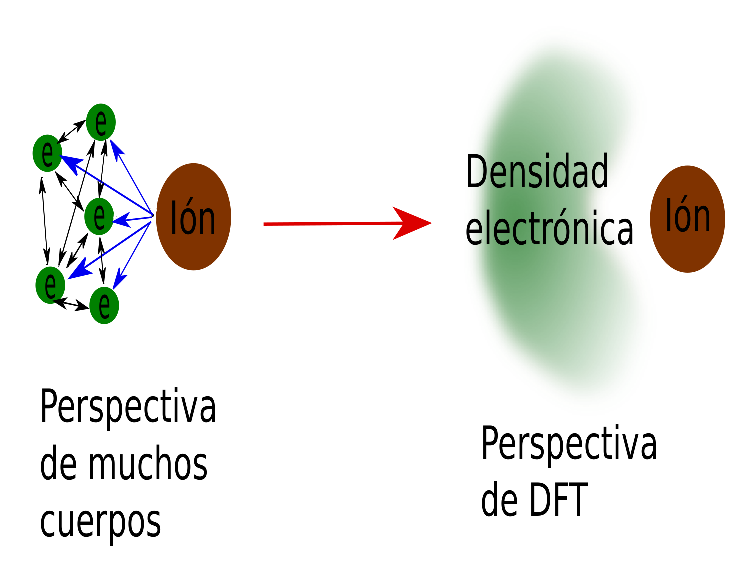
\includegraphics[width=7.0cm,height=7.0cm]{figuras/perspectivaDFT.eps}
  	\caption[Perspectiva de la teor\'ia Funcional de la Densidad.]{Idea de la Teor\'ia Funcional de la Densidad que consiste en sustituir las interacciones de muchos cuerpos con una interacci\'on promedio por medio de una densidad electr\'onica. \cite{MB-2015}}
  	\label{im:dftIdea}
  \end{figure}
  
  La teor\'ia desarrollada por Hohenberg y Kohn \cite{HK-1964} para una formulaci\'on de DFT como una teor\'ia exacta de un sistema de muchos cuerpos  solo es v\'alida para su estado base por lo tanto  es importante encontrar los valores de expectaci\'on en funci\'on los estados base $\Psi_0$ para la energ\'ia, la densidad electr\'onica y la  magnetizaci\'on  (Ecs. \ref{ec:energia}, \ref{ec:denspin} y \ref{ec:magn}, respectivamente). Es importante separar el Hamiltoniano  de la ecuaci\'on \ref{ec:shelectron} como:
  \begin{equation}
  \hat{H} =\hat{H}_0 + \hat{H}_{ext}, \label{ec:sepHamilton}
  \end{equation}
  en donde $\hat{H}_0 = \hat{T}+\hat{V}_{int}$ y $\hat{H}_{ext}= \hat{V}_{ext} + E_{II}$.  Cuando se desea considerar el aporte de la magnetizaci\'on es necesario agregar una interacci\'on de estilo Zeeman de un campo magn\'etico externo 
  $-\pmb{B}_{ext} (\pmb{r}) \cdot \pmb{m} (\pmb{r}).$\cite{Martin-2004} 
  Este potencial es valido debido a que solo se considera el aporte de la magnetizaci\'on del spin y se puede considerar el potencial de interacci\'on debido a fuentes externas \cite{MB-2015, Martin-2004} como 
  \begin{equation}
  \hat{H}_{ext} = \hat{V}_{Ex}^{s', s} = \hat{V}_{ext} \delta_{s',s} - \pmb{B}_{ext} (\pmb{r})\cdot \pmb{m} (\pmb{r}) +E_{II}. \label{ec:intExt}
  \end{equation}
  En caso de que se trabaje con una orientaci\'on no colineal, es necesario agregar el t\'ermino de acople spin-\'orbita al campo magn\'etico externo \cite{MB-2015}:
  \begin{equation}
  \pmb{B}_{ext} (\pmb{r}) \to  \pmb{B}_{ext} (\pmb{r}) + \frac{i \hbar^2}{\mu_{B} (2 m c)^2} \{[\nabla V_{ext}]\times \nabla \}.
  \label{ec:Spinorb}\end{equation}
  \newline
  La teor\'ia desarrollada muestra que el funcional de la energ\'ia est\'a caracterizado por la densidad de electrones (Ec. \ref{ec:densidadr}) y la magnetizaci\'on (Ec. \ref{ec:magn}) \cite{PhysRevB.37.10685}:
  \begin{equation}
  E=E_{V_{ext}, \pmb{B}_{ext}} [n,\pmb{m}]. \label{ec:func1}
  \end{equation}
\newline
  \par El primer teorema de Hohenberg y Kohn se relaciona con el hecho  de que el potencial externo dado por la Ec. \ref{ec:intExt}  est\'a determinado \'unicamente por la densidad y la magnetizaci\'on en el estado base $n_0$ y $\pmb{m}_0$. Esto se muestra en la figura \ref{fig:hk1},   en donde las flechas azules muestran la soluci\'on que usualmente se sigue para resolver la ecuaci\'on de Schrödinger y la flecha roja indica la relaci\'on establecida por el primer teorema de Hohenberg-Kohn.  Como consecuencia de este teorema dos estados base distintos $\Psi_0 $ y $\Psi_0 '$ dan lugar a dos matrices de densidad de spines diferentes $n_{s',s} \not =n_{s',s}' $ y por lo tanto $n(\pmb{r}), \pmb{m}(\pmb{r}) \not = n'(\pmb{r}), \pmb{m}'(\pmb{r})$. Debido a este teorema es posible determinar las funciones de muchos cuerpos para todos los niveles sin importar que est\'en desocupados y entonces todas las propiedades del sistema se pueden determinar teniendo s\'olo la densidad de electrones en el estado base \cite{HK-1964, PhysRevB.37.10685}.
  \begin{figure}[!hbt]
  	\centering
  	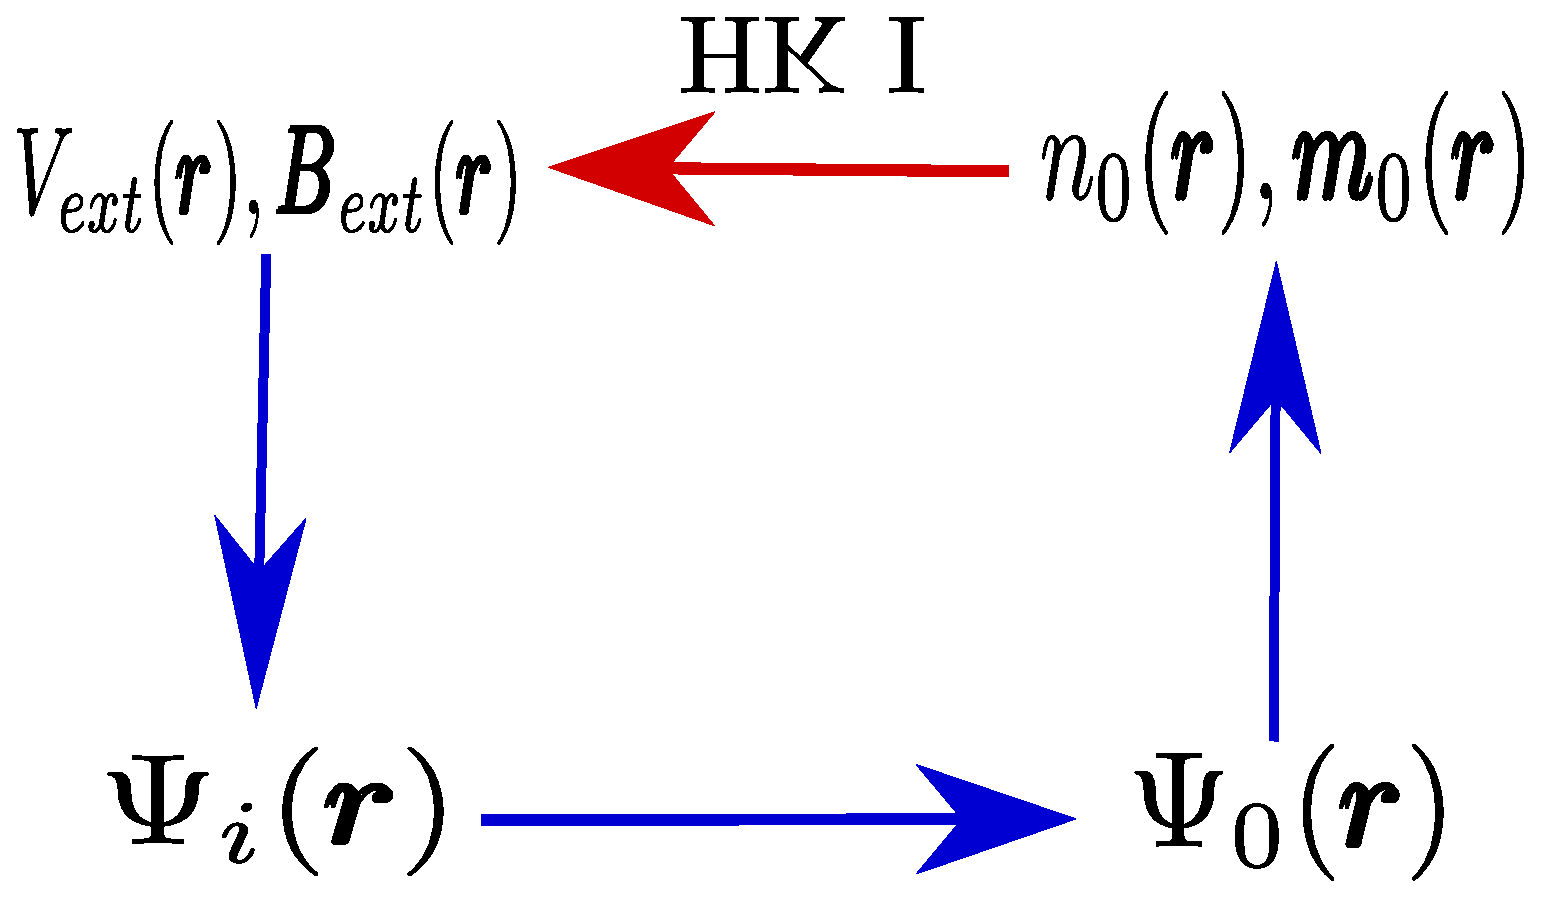
\epsfig{file=figuras/HK1.eps, width=8.0cm,height=5.0cm}
  	\caption[Primer teorema de Hohenberg-Kohn]{Representaci\'on esquem\'atica del primer teorema de Hohenberg-Kohn}
  	\label{fig:hk1}
  \end{figure}


%  \newline
  \par El segundo teorema esta relacionado con la posibilidad de determinar un funcional para la energ\'ia $E_{V_{ext}, \pmb{B}_{ext}}[n,\pmb{m}]$ en t\'erminos de la densidad y la magnetizaci\'on que es v\'alido para cualquier potencial externo $\hat{V}_{Ex}^{s', s}$. Para un $\hat{V}_{Ex}^{s', s}$ particular, la energ\'ia del estado base del sistema es el m\'inimo global de este funcional y la densidad $n(\pmb{r})$ y la magnetizaci\'on $\pmb{m}(\pmb{r})$ que minimizan el funcional son los par\'ametros exactos para el estado base  $n_0(\pmb{r})$ y $\pmb{m}_0(\pmb{r})$. Este potencial se puede escribir como \cite{PhysRevB.37.10685}
  \begin{equation}
   E_{V_{ext}, \pmb{B}_{ext}}[n,\pmb{m}]= F[n,\pmb{m}] + \int d \pmb{r} \{V_{ext} (\pmb{r}) n(\pmb{r})+\pmb{B}_{ext} (\pmb{r}) \cdot \pmb{m} (\pmb{r}) \} +E_{II}, \label{ec:funcional}
  \end{equation}
  en donde$F[n,\pmb{m}]$ es el llamado funcional universal el cual incluye las energ\'ias cin\'eticas y potencial del sistema de electrones:
  \begin{eqnarray}
  F[n,\pmb{m}]&= \langle \Psi_0 [n,\pmb{m}]| \hat{T}+\hat{V}_{int} | \Psi_0 [n,\pmb{m}] \rangle \nonumber \\
              &= T[n,\pmb{m}] + V_{int} [n,\pmb{m}]. \label{ec:funcF}
  \end{eqnarray}
  
  Si se considera  la densidad $n_0 (\pmb{r})$ y la magnetizaci\'on $\pmb{m}_0  (\pmb{r})$ del estado base, se puede determinar la energ\'ia
  \begin{equation}
  E_0= E_{V_{ext}, \pmb{B}_{ext}}[n_0,\pmb{m}_0], \label{ec:estadoBase}
  \end{equation}
  la cual obedece la desigualdad
  \begin{equation}
  E_0 < E_{V_{ext}, \pmb{B}_{ext}}[n,\pmb{m}], \label{ec:desig}
  \end{equation}
  en donde $ n (\pmb{r}),\pmb{m} (\pmb{r}) \not = n_0 (\pmb{r}),\pmb{m}_0 (\pmb{r})$. Tomando esto en consideraci\'on  se puede establecer el segundo  teorema de Hohenberg-Kohn como sigue \cite{MB-2015}:
  \begin{equation}
  E_0 = \min_{n  \to n_0, \pmb{m} \to \pmb{m}_0} E_{V_{ext}, \pmb{B}_{ext}}[n,\pmb{m}]  \label{ec:HKII}.
  \end{equation}
  Por consecuencia de este segundo teorema, el funcional de la Ec. \ref{ec:funcional} es suficiente para determinar la energ\'ia del estado base as\'i como su densidad y magnetizaci\'on. En la siguiente secci\'on se mostrar\'a el proceso general para encontrar estos valores por medio de las ecuaciones de Kohn-Sham, adem\'as que se mostrar\'a la raz\'on por la que se les llama evaluaci\'on auto consistente.
  
  \section{Ecuaciones de Kohn-Sham} \label{sec:KSH}
   Las ecuaciones de Kohn-Sham representan un sistema de ecuaciones auxiliares para resolver el problema de muchos cuerpos que representa el Hamiltoniano de la Ec. \ref{ec:sh}. Estos autores propusieron que la densidad y la magnetizaci\'on del estado base pueden ser representados con un sistema auxiliar para part\'iculas sin interacci\'on, en donde el Hamiltoniano auxiliar se elige de tal forma que el operador de  energ\'ia cin\'etica $ \hat{T}$ y el potencial local $ V_{eff}^s $ act\'uan sobre un electr\'on con spin $s$ en la posici\'on $\pmb{r}$. Tal Hamiltoniano del sistema auxiliar se puede escribir como (en unidades de Hartree) \cite{Martin-2004}:
  \begin{equation}
  \hat{H}_{aux}^{s} = - \frac{1}{2} \nabla^2 + V_{eff}^s (\pmb{r}). \label{ec:HAux}
  \end{equation}  
  Si se considera un sistema de spines colineales,  el n\'umero de electrones independientes es $N = N_{\uparrow}+ N_{\downarrow}$ y la densidad de electrones en este sistema est\'a dada por la Ecuaci\'on \ref{ec:denspin} con $s' = s$ de tal forma que la energ\'ia cin\'etica de una sola part\'icula $T_{sp}$, en donde no existe ning\'un potencial, se define como \cite{MB-2015}:
  \begin{equation}
  T_{sp} = -\frac{1}{2} \sum_{s} \sum_{i} n_{i,s} \int d^3 r ~\psi_{i,s }^* (\pmb{r}) \nabla^2 \psi_{i,s } (\pmb{r})  = \frac{1}{2} \sum_{s} \sum_{i} n_{i,s} \int d^3 r  |\nabla \psi_{i,s } (\pmb{r}) |^2 .\label{ec:funCinetica}
  \end{equation}
    Por lo tanto se puede reescribir la funcional de la Ec. \ref{ec:funcional} sin considerar campos magn\'eticos externos como: 
   \begin{equation}
   E_{KS}[n] = T_{sp}[n]+ \int d \pmb{r} V_{ext} (\pmb{r}) n_s (\pmb{r}) +E_{Hartree} [n] + E_{XC}^s [n] + E_{II}. \label{ec:funcHK}
   \end{equation}
    Los efectos de intercambio y correlaci\'on se agrupan en $E_{XC}^s [n]$, el cual se puede escribir en t\'erminos del funcional de Hohenberg-Kohn (ec. \ref{ec:funcional}) \cite{Martin-2004} :
   %\begin{equation}
   %E_{XC}^s [n] = F[n]-(T_{sp} [n]+E_{Hartree}[n]) \label{ec:eXC2}
   %\end{equation}
   %la cual se puede reescribir como:
   \begin{equation}
   E_{XC}^s [n]= \langle \hat{T} \rangle - T_{sp} [n]+\langle \hat{V}_{int} \rangle-E_{Hartree} [n] \label{ec:Exc2},
   \end{equation}
    en donde se observa que la energ\'ia de intercambio y correlaci\'on no solo depende de la diferencia entre las interacciones de Coulomb ($\langle \hat{V}_{int} \rangle-E_{Hartree}[n]$), sino que tambi\'en por la diferencia entre la energ\'ia cin\'etica entre el sistema con interacciones y el que no las tiene ($ \langle \hat{T} \rangle - T_{sp} [n] $) \cite{MB-2015}.
   \newline
   \par Para cumplir con el segundo teorema de Hohenberg y Kohn, se minimiza el funcional de la energ\'ia (ec. \ref{ec:funcHK}) con respecto  a las funciones de los orbitales $\psi_{i,s } $: 
   \begin{equation}
   \frac{\delta E_{KS} [n_s]}{\delta \psi_{i,s } ^* (\pmb{r})}= \frac{\delta T_{sp} }{\delta \psi_{i,s } ^* (\pmb{r}) } + \left[\frac{\delta E_{ext}}{\delta n_s (\pmb{r})}+\frac{\delta E_{Hartree}}{\delta n_s (\pmb{r})}+  \frac{\delta E_{XC}^s}{\delta n_s (\pmb{r})}\right] \frac{\delta n_s (\pmb{r})}{\delta \psi_{i,s } ^* (\pmb{r})} =0. \label{ec:ecEulerFun}
   \end{equation}
   Utilizando las ecuaciones \ref{ec:denspin} y \ref{ec:funCinetica} se obtiene lo siguiente:
   \begin{equation}
   \frac{\delta T_{sp} }{\delta \psi_{i,s } ^* (\pmb{r}) }= -\frac{1}{2} \nabla^2 \psi_{i,s } (\pmb{r}); ~~ \frac{\delta n_s (\pmb{r})}{\delta \psi_{i,s } ^* (\pmb{r})}= \psi_{i,s } (\pmb{r}) \label{ec:simp};
   \end{equation} 
   adem\'as sustituyendo  la Ec. \ref{ec:simp} en \ref{ec:ecEulerFun}    y utilizando el m\'etodo de los multiplicadores de Lagrange  sujeto a la condici\'on $\langle \psi_{i,s} | \psi_{j,s'} \rangle =   \delta_{i,j}\delta_{s',s}$,   se obtiene la ecuaci\'on de Kohn-Sham:
   \begin{equation}
   (H_{KS}^s -\epsilon_{i,s})\psi_{i,s } (\pmb{r}) = 0 \label{ec:ShKS},
   \end{equation}
   en donde $ H_{KS}^s $ es el Hamiltoniano efectivo definido por \cite{PhysRev.140.A1133}:
   \begin{equation}
    H_{KS}^s = -\frac{1}{2} \nabla^2 + V_{KS}^s (\pmb{r}), \label{ec:HamiltonianoKS}
   \end{equation}
   con
   \begin{eqnarray}
     V_{KS}^s (\pmb{r}) &=& V_{ext} (\pmb{r})+  \frac{\delta E_{Hartree}}{\delta n_s (\pmb{r})}+  \frac{\delta E_{XC}^s}{\delta n_s (\pmb{r})} \nonumber \\
      &=& V_{ext} (\pmb{r})+ V_{Hartree} (\pmb{r}) + V_{XC}^s (\pmb{r}). \label{ec:potKS} 
   \end{eqnarray}
   Las Ecs. \ref{ec:ShKS} y \ref{ec:potKS} conforman las ecuaciones de Kohn-Sham y las cuales tienen que ser resueltas auto consistentemente con el c\'alculo de la densidad (Ec. \ref{ec:denspin}) y la energ\'ia total (Ec. \ref{ec:funcHK}). La evaluaci\'on  auto consistente para el caso de spines colineales se muestra en la figura \ref{fig:esq}, en donde se resuelven para dos orientaciones de spines $\uparrow, \downarrow$. El proceso inicia calculando la densidad de electrones considerando que los \'atomos est\'an aislados, despu\'es se compara la energ\'ia de Kohn-Sham con la iteraci\'on anterior y, si la diferencia es casi cero entonces se dice que el calculo de energ\'ia ha convergido y termina la ejecuci\'on, en caso contrario se vuelve a calcular la densidad con las funciones de onda calculadas anteriormente y se repite el proceso. 
   \begin{figure}[!hbt]
   	\centering
   	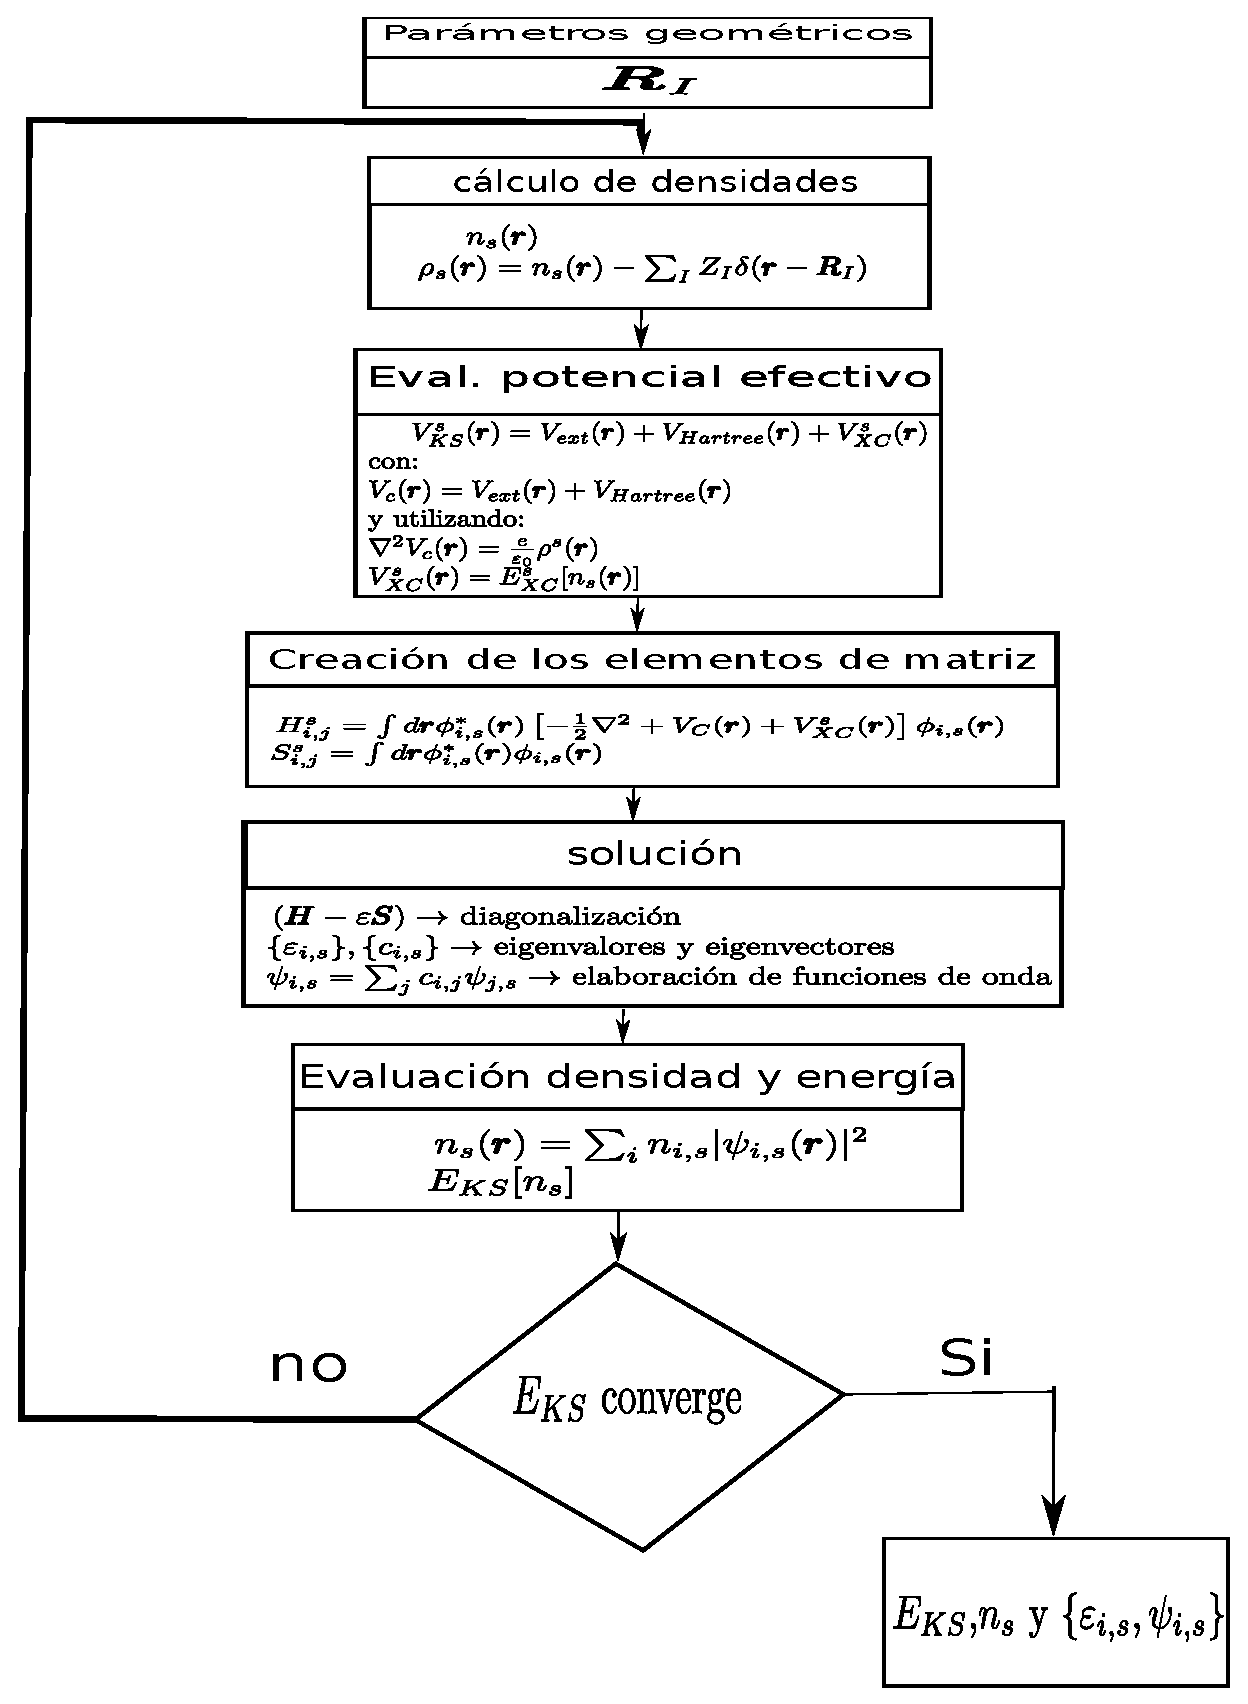
\epsfig{file=figuras/diagramaAuto.eps, width=15.0cm,height=19cm}
   	\caption[Diagrama de evaluaci\'on auto consistente]{Ciclo para resolver de forma auto consistente las ecuaciones de Kohn-Sham.}
   	\label{fig:esq}
   \end{figure}
   \newline
   \par En el caso de los spines no colineales no es posible separar la funci\'on de onda $\phi_{\Lambda} (\pmb{r},s)\not = \psi_{i,s } (\pmb{r}_j) \alpha_i (s_j) $, en donde $\Lambda$ representa los n\'umeros cu\'anticos  del orbital. Tambi\'en es necesario agregar un nuevo t\'ermino a la ecuaci\'on \ref{ec:ShKS} llamado campo magn\'etico de intercambio y correlaci\'on \cite{PhysRevB.37.10685}:
   \begin{equation*}
   B_{XCj} (\pmb{r}) = - \frac{\delta E_{XC} [n,\pmb{m}]}{\delta m_j (\pmb{r})} \label{ec:Bxc},
   \end{equation*}
   el cual representa un campo magn\'etico interno inducido por  los efectos de intercambio y correlaci\'on y en lugar de un sistema de dos ecuaciones  para el caso colineal, se tiene que resolver un sistema de cuatro ecuaciones \cite{MB-2015}:
   \begin{multline}
   \sum_{s}  \left[-\frac{1}{2} \nabla^2 + V_{ext} (\pmb{r})+ V_{Hartree} (\pmb{r}) + V_{XC} (\pmb{r}) \right] \delta_{s',s}  \phi_{\Lambda} (\pmb{r},s)\\ - \mu_{B} \sum_{s}  [\pmb{B}_{ext} (\pmb{r})+ \pmb{B}_{XC} (\pmb{r}) ] \cdot \pmb{\sigma_{s,s'}} \phi_{\Lambda} (\pmb{r},s) = \varepsilon_{\Lambda} \phi_{\Lambda} (\pmb{r},s) , \label{ec:KSnoColl}
   \end{multline}
   en donde $s$ toma los valores de $\uparrow, \downarrow$ y  las dos componentes del spinor correspondiente a cada orientaci\'on. As\'i mismo hay que considerar el acople spin \'orbita tal como se muestra en la secci\'on \ref{sec:Ho-Ko}.
   \subsection{Evaluaci\'on no auto consistente} \label{subsec:nscf}
   Cuando es necesario calcular estructuras de bandas o la densidad de estados, se utiliza una red mas densa en el espacio rec\'iproco (Sec. \ref{sec:solespacioK}). En este caso no es pr\'actico realizar el ciclo auto consiente y entonces lo que se hace es tomar la densidad de carga obtenida por la evaluaci\'on auto consistente con un n\'umero menor de puntos en el espacio rec\'iproco  y resolver la ecuaciones de Kohn-Sham (Ecs. \ref{ec:ShKS}-\ref{ec:potKS}), con el n\'umero de puntos en el espacio rec\'iproco deseado y obteniéndose así  una nueva densidad $n_0$,  dado que puede variar la magnitud de la densidad obtenida por este m\'etodo con respecto al que se obtiene con una evaluaci\'on auto consistente, se utiliza el  funcional de Harris  para evaluar la energ\'ia total del sistema debido a que es menos sensible a los cambios en $n_0$ que el potencial de Kohn-Sham. Este funcional est\'a dado por\cite{PhysRevB.31.1770}:
   \begin{equation}
   E_{Harris} [n_0] = \sum_{i} \varepsilon_i - \int d^3 r V_{ext} [n_0] n_0 (\pmb{r}) - \frac{1}{2} \int d^3 r V_{Hartree} [n_0] n_0 (\pmb{r}) + E_{XC} [n_0]. \label{ec:FuncHarris}
   \end{equation}
  
   \section{Funcional de intercambio y correlaci\'on ($E_{XC} $)}\label{sec2:xc}
   \subsection{Propiedades del funcional $E_{XC} $ exacto } \label{susec:exXC}
   El funcional de la energ\'ia de intercambio y correlaci\'on (Ec. \ref{ec:Exc2} )  se puede escribir como \cite{MB-2015}:
   \begin{equation}
   E_{XC}^s [n_s] = \int d \pmb{r} n_s (\pmb{r}) \epsilon_{XC} (\pmb{r}; [n_s]) \label{ec:enGenXCf},
   \end{equation} 
   donde $ \epsilon_{XC} (\pmb{r}; [n_s])$ es la energ\'ia de intercambio y correlaci\'on por part\'icula; en el caso de que los spines no est\'en orientados colinealmente se tiene que considerar la magnetizaci\'on y la polarizaci\'on.
   \newline
   \par Para analizar la contribuci\'on de $E_{XC} $ se utiliza el m\'etodo de conexi\'on adiab\'atica \cite{PhysRevA.29.1648}, en el que el cambio de la energ\'ia del sistema con respecto al par\'ametro $\lambda$ es igual al elemento de matriz de la derivada del Hamiltoniano con respecto al mismo par\'ametro. Entonces se puede calcular la energ\'ia entre dos estados $\lambda_1$ y $\lambda_2$ a través de una integral sobre una variaci\'on  del Hamiltoniano, que var\'ie de  $\lambda_1$ a $\lambda_2$. La denominaci\'on  de conexi\'on adiab\'atica se debe a que se asume que el Hamiltoniano que conecta los dos estados est\'a en el estado base para el valor de $\lambda$ y las expresiones generales son  dadas por \cite{Martin-2004, PhysRevA.29.1648}:
   \begin{equation}
   \frac{\partial E_0}{\partial \lambda} = \frac{\partial}{\partial \lambda} \left \langle \Psi_0^{\lambda} \left | \hat{H}_0 ^{\lambda} \right |  \Psi_0^{\lambda} \right \rangle = \left \langle \Psi_0^{\lambda} \left | \frac{\partial \hat{H}_0 ^{\lambda}}{\partial \lambda} \right |  \Psi_0^{\lambda} \right \rangle \label{ec:adAproxderivada}
   \end{equation}  
   o escrito en forma de integral:
   \begin{equation}
   \Delta E_0 = \int_{\lambda_1}^{\lambda_2} d \lambda~ \frac{\partial E_0}{\partial \lambda} = \int_{\lambda_1}^{\lambda_2} d \lambda \left \langle \Psi_0^{\lambda} \left | \frac{\partial \hat{H}_0 ^{\lambda}}{\partial \lambda}  \right |  \Psi_0^{\lambda} \right \rangle \label{ec:adAproxInt}.
   \end{equation}
   Se  escala el t\'ermino de la interacci\'on entre electrones $\lambda \hat{V}_{int}$ con el par\'ametro $\lambda (0 \le \lambda \le 1)$ entre un sistema sin interacci\'on ($\lambda=0$) y uno con interacci\'on ($\lambda=1$) y  se asume que $n(\pmb{r})= n^{\lambda} (\pmb{r})$, entonces es posible definir el siguiente Hamiltoniano \cite{Harris1974TheSE}: 
   \begin{equation}
   \hat{H}_{0}^{\lambda} = \hat{T}+ \hat{V}_{ext}^{\lambda}+ \lambda \hat{V}_{int} \label{ec:SH1Elec},
   \end{equation}
   en donde se reemplaza el potencial externo $\hat{V}_{ext} $ con $\hat{V}_{ext}^{\lambda} $ para garantizar que no cambie la densidad, utilizando las ecuaciones \ref{ec:adAproxderivada} y \ref{ec:adAproxInt} se puede escribir el funcional de la energ\'ia del estado base (Ec. \ref{ec:funcional} con $\pmb{B}_{ext}=0$) como  \cite{MB-2015}:
   \begin{subequations}
   	\begin{equation*}
   	E_0 = E_{V_{ext}} [n] = \langle \Psi_0^1 | \hat{H}_0 ^ 1 | \Psi_0^1 \rangle
   	\end{equation*}
   	\begin{equation*}
   	=\langle \Psi_0^0 | \hat{H}_0 ^ 0 | \Psi_0^0 \rangle + \int_{0}^{1} d \lambda \frac{\partial}{\partial \lambda } \left \langle \Psi_0^{\lambda} \left | \hat{H}_0 ^{\lambda} \right |  \Psi_0^{\lambda} \right \rangle
   	\end{equation*}
   	\begin{equation*}
   	=\langle \Psi_0^0 | \hat{H}_0 ^ 0 | \Psi_0^0 \rangle + \int d \pmb{r} [V_{ext}^1 (\pmb{r})-V_{ext}^0 (\pmb{r})] n (\pmb{r}) + \int_{0}^{1} d \lambda  \left \langle \Psi_0^{\lambda} \left | \hat{V}_{int} \right |  \Psi_0^{\lambda} \right \rangle
   	\end{equation*}
   \end{subequations}
   y asumiendo  que $V_{ext}^1 (\pmb{r}) \equiv V_{ext} (\pmb{r})$:
   \begin{equation*}
   E_0 = E_{V_{ext}} [n]= \langle \Psi_0^0 | \hat{T} | \Psi_0^0 \rangle + \int d \pmb{r} V_{ext} (\pmb{r}) n (\pmb{r}) + \int_{0}^{1} d \lambda  \left \langle \Psi_0^{\lambda} \left | \hat{V}_{int} \right |  \Psi_0^{\lambda} \right \rangle ;
   \end{equation*}
   dado que el primer t\'ermino corresponde a $T_{sp}$, se puede encontrar una nueva expresi\'on para $E_{XC}$ \cite{Martin-2004}: 
   \begin{equation}
   E_{XC} [n] = \int_{0}^{1} d \lambda  \left \langle \Psi_0^{\lambda} \left | \hat{V}_{int} \right |  \Psi_0^{\lambda} \right \rangle-E_{Hartree} = \frac{1}{2} \int d \pmb{r} n(\pmb{r})\int d \pmb{r'}  \frac{\widetilde{n }_{xc}(\pmb{r},\pmb{r'})}{|\pmb{r}-\pmb{r'}|} \label{ec:Exc3},
   \end{equation}
   en donde $\widetilde{n }_{xc} (\pmb{r},\pmb{r'})$ se define como \cite{Martin-2004}:
   \begin{equation}
   \widetilde{n }_{xc} (\pmb{r},\pmb{r'}) = \int_{0}^{1} d \lambda n_{xc}^{\lambda} (\pmb{r},\pmb{r'}) \label{ec:avHole}.
   \end{equation}
   Las ecuaciones \ref{ec:enGenXCf} y \ref{ec:Exc3} se utilizan para  escribir la energ\'ia de intercambio y correlaci\'on por part\'icula $\epsilon_{XC} $ como:
   \begin{equation}
   \epsilon_{XC} (\pmb{r}; [n])= \frac{1}{2} \int d \pmb{r'}  \frac{\widetilde{n }_{xc}(\pmb{r},\pmb{r'})}{|\pmb{r}-\pmb{r'}|} \label{ec:densEXC}.
   \end{equation}
     Se puede expresar el potencial de intercambio y correlaci\'on en funci\'on de la energ\'ia de intercambio y correlaci\'on por part\'icula \cite{PhysRevA.29.1648} como:
   \begin{equation}
   V_{XC} (\pmb{r}) = \epsilon_{XC} (\pmb{r}; [n]) + n(\pmb{r}) \frac{\delta \epsilon_{XC} (\pmb{r}; [n])}{\delta n(\pmb{r}) } \label{ec:potXC}.
   \end{equation}  
   La generalizaci\'on para el caso de spines colineales es \cite{Martin-2004}:
   \begin{equation}
   V_{XC}^s (\pmb{r}) = \epsilon_{XC} (\pmb{r}; [n]) + n(\pmb{r}) \frac{\delta \epsilon_{XC} (\pmb{r}; [n])}{\delta n_s(\pmb{r}) } , \label{ec:potXCspin}
   \end{equation}
   en donde se toma en cuenta que $\epsilon_{XC} \equiv \epsilon_{XC} \left(\pmb{r}; \left[ n_{\uparrow}, n_{\downarrow} \right]\right) $ es un funcional de las dos densidades de spines.
\newline
   \par Una de las primeras aproximaciones que se realizaron a la energ\'ia de intercambio y correlaci\'on fue la aproximaci\'on local de la densidad (LDA, por sus siglas en ingl\'es) \cite{PhysRev.140.A1133}, la cual presenta errores tales como la sobre estimaci\'on de  las energ\'ias de cohesi\'on de casi todos ls s\'olidos; adem\'as de la subestimaci\'on de los par\'ametros de red en varios casos, as\'i como  los errores al momento de describir sistemas altamente correlacionados y en especial presenta problemas con \'atomos de metales de transici\'on \cite{MB-2015}. Una forma de corregir estos inconvenientes es incluir correcciones de gradientes de la densidad para que la energ\'ia de intercambio y correlaci\'on pueda ser escrita en funci\'on de una densidad de energ\'ia de intercambio y correlaci\'on $g_{r} [n]$ \cite{MB-2015}:
   \begin{equation}
   E_{XC} [n]= \int d^3~ r g_{r} [n]
   \end{equation}
   y esta densidad se puede expandir en series \cite{PhysRevLett.22.807}:
$
   g_{r} [n] = g_0 (n(\pmb{r}))+ g_1 (n(\pmb{r})) [\nabla n(\pmb{r})]+ \ldots~
 .$
   Dicha  teor\'ia fue propuesta por Kohn y Sham\cite{PhysRev.140.A1133} aunque \'esta no soluciona los principales problemas de LDA. Por tal motivo se implement\'o la aproximaci\'on de gradientes generalizados (GGA, por sus siglas en ingl\'es) cuya expresi\'on para la energ\'ia de intercambio y correlaci\'on est\'a dada por \cite{Perdew1996ComparisonSF}:
   \begin{multline}
      E_{XC}^{GGA} [n_{\uparrow} (\pmb{r}), n_{\downarrow}(\pmb{r})] = \int d^3 r ~ n(\pmb{r}) \epsilon_{XC} \left(n_{\uparrow} (\pmb{r}), n_{\downarrow}(\pmb{r}), \left|\nabla n_{\uparrow} (\pmb{r}) \right|^2, \left|\nabla n_{\downarrow} (\pmb{r}) \right|^2 \right)  \\
      = \int d^3 r ~ n(\pmb{r}) \epsilon_{X}^{hom} (n) F_{XC} \left(n_{\uparrow} (\pmb{r}), n_{\downarrow}(\pmb{r}), \left|\nabla n_{\uparrow} (\pmb{r}) \right|^2, \left|\nabla n_{\downarrow} (\pmb{r}) \right|^2 \right), \label{ec:funcXCGGA}
   \end{multline}
   en donde $ \epsilon_{X}^{hom} (n) = -3k_F / 4\pi $ es la energ\'ia de intercambio por part\'icula  de un gas de electrones homog\'eneo no polarizado y  $k_F = (3 \pi^2 n)^{1/3}$ es el vector de onda de Fermi y $F_{XC}$ es una funci\'on adimensional de las densidades y sus gradientes \cite{Martin-2004}. Dicha funcional \ref{ec:funcXCGGA} se denota un funcional XC semilocal. Es importante tomar en cuenta que es posible separar la parte correspondiente a la correlaci\'on de la de intercambio de la siguiente manera: $ \epsilon_{XC} (\pmb{r}; [n] )= \epsilon_{X} (\pmb{r}; [n] )+ \epsilon_{C} (\pmb{r}; [n] ) $ y por lo tanto tambi\'en es v\'alido realizar la siguiente divisi\'on $ F_{XC} = F_{X}+ F_{C} $ \cite{MB-2015}.
   \newline
   \par Una de las aproximaciones mas utilizadas es la desarrollada por Perdew, Burke y Enzerhof (PBE) en donde la parte correspondiente a el intercambio puede ser escrita de la siguiente forma \cite{PhysRevLett.77.3865, mo_2004}:
   \begin{equation}
   E_X [n_{\uparrow}, n_{\downarrow}]= \frac{1}{2} \left[E_{X} [2 n_{\uparrow}] + E_{X} [2 n_{\downarrow}]   \right]. \label{ec:divEx}
   \end{equation}
   Adem\'as se puede definir el gradiente de densidad reducida como:
   \begin{equation}
   s(\pmb{r})= \frac{|\nabla n (\pmb{r})|}{2 k_F n (\pmb{r}) }. \label{ec:S}
   \end{equation}
   Por tanto  $F_X (s)$ queda dada por:
   \begin{equation}
   F_{X}^{PBE} = 1+\kappa -\frac{\kappa}{1+\mu s^2 /\kappa}, \label{ec:F_X-PBE}
   \end{equation}
   donde $\mu = 0.21951 $ y $\kappa= 0.804 $. La energ\'ia de correlaci\'on est\'a dada por \cite{mo_2004}:
   \begin{equation}
   E_{C} ^{PBE} = \int d^3 r n \left\{\epsilon_{C}(r_s,\zeta)+ H^{PBE} (r_s,\zeta,t), \right\}\label{ec:funcCorr},
   \end{equation}
   donde $r_s = (3/4 \pi n)^{1/3}, ~ \zeta =(n_{\uparrow}-n_{\downarrow})/n,~ t=|\nabla n|/2 k_s \phi n, ~\phi= \frac{1}{2} [(1+\zeta)^{2/3}+(1-\zeta)^{2/3}],~ k_s = (4 k_F/\pi)^{1/2}$,
   \begin{equation}
   H^{PBE} = \gamma \phi^3 \ln \left\{1+ \frac{\beta}{\gamma} t^2 \left[\frac{1+At^2}{1+At^2+A^2 t^4}\right]\right\}, \label{ec:PBEH}
   \end{equation}
   \begin{equation}
   A=\frac{\beta}{\gamma} [exp\{-\epsilon_{C}^{hom}/\gamma \phi^3 \}-1]^{-1} \label{ec:A}
   \end{equation}
   y $\gamma=0.031091, ~\beta=0.066725$. Los gradientes reducidos $s$ y $t$ miden qu\'e tan r\'apido $n(\pmb{r})$ var\'ia en las escalas de la longitud de onda de Fermi $2\pi/k_F$ y el apantallamiento de Thomas-Fermi $1/k_s$ respectivamente. Esta clase de funcionales mejoran los resultados obtenidos con LSDA \cite{MB-2015}.
   \newline
   \par Para calcular el potencial de intercambio y correlaci\'on encontrando el cambio $\delta E_{XC} [n]$ con respecto a un cambio  $\delta n$ y $\nabla \delta n$, se usa la siguiente expresi\'on \cite{Martin-2004}:
   \begin{equation}
   \delta E_{XC} [n] = \sum_{s} \int d \pmb{r} \left[\epsilon_{XC} + n \frac{\partial \epsilon_{XC}}{\partial n_s} + n \frac{\partial \epsilon_{XC}}{\partial \nabla n_s} \right]_{\pmb{r},s} \delta n_s(\pmb{r}), \label{ec:ecpotVXC_1}
   \end{equation}
   en donde el termino dentro de los par\'entesis cuadrados no se puede considerar como un potencial local debido al \'ultimo t\'ermino. Existen tres aproximaciones para manejar este t\'ermino, la primera es encontrar el potencial local $V_{XC}^s (\pmb{r})$ por interacci\'on  del \'ultimo  t\'ermino \cite{Martin-2004}:
   \begin{equation}
   V_{XC}^s (\pmb{r}) = \left[\epsilon_{XC}+\frac{\partial \epsilon_{XC}}{\partial n_s}- \nabla \left(n \frac{\partial \epsilon_{XC}}{\partial \nabla n_s}\right) \right] \label{ec:potXC_2},
   \end{equation}
   el cual es el mas usado pero tiene como desventaja que requiere derivadas de mayor orden para la densidad, lo cual crea dificultades num\'ericas.
   \newline
   \par La segunda aproximaci\'on es usar un operador de la forma dada por ecuaci\'on \ref{ec:potXC} directamente para modificar las ecuaciones de Kohn-Sham. Usando el hecho de que la densidad se puede escribir en t\'erminos de las funciones de onda $\psi_i$, el elemento de matriz quedar\'ia como \cite{PhysRevLett.76.660}:
   \begin{equation}
   \langle \psi_i |\hat{V}_{XC}| \psi_i \rangle = \int \left[\tilde{V}_{XC} \psi_i ^* \psi_i + \psi_i ^* \pmb{V}_{XC} \cdot \nabla \psi_i + (\pmb{V}_{XC} \cdot \nabla \psi_i^*) \psi_i \right], \label{ec:potXC_3}
   \end{equation}
   donde $\tilde{V}_{XC} = \epsilon_{XC} + n (\partial \epsilon_{XC}/ \partial n)$ y $\pmb{V}_{XC} = n (\partial \epsilon_{XC} / \partial \nabla n) $. Esta forma es mas estable en t\'erminos num\'ericos pero requiere la inclusi\'on de operaciones vectoriales en la ecuaci\'on de Kohn-Sham lo cual incrementa  el respectivo trabajo computacional \cite{Martin-2004}.
   \newline
   \par Finalmente, la tercera aproximaci\'on fue propuesta por White y Bird \cite{PhysRevB.50.4954} que consiste en tratar $E_{XC}$ como una funci\'on de la densidad, donde los t\'erminos de  los gradientes son definidos por un operacional en funci\'on de la densidad. Entonces la ecuaci\'on \ref{ec:potXC} puede ser escrita usando la regla de la cadena:
   \begin{multline}
   \delta E_{XC} [n] = \sum_{s} \int d \pmb{r} \left[\epsilon_{XC} + n \frac{\partial \epsilon_{XC}}{\partial n_s} \right] \delta n_s (\pmb{r}) \\
   + \sum_{s}  \int\int d  \pmb{r} d \pmb{r'} n(\pmb{r}) \left[\frac{\partial \epsilon_{XC}}{\partial \nabla n_s} \right] ~ \frac{\delta \nabla n(\pmb{r'})}{\delta n(\pmb{r})} \delta n_s (\pmb{r}), \label{ec:potXC_4}
   \end{multline}
   donde $ (\delta n(\pmb{r'})/\delta n(\pmb{r}))$ denota una derivada funcional. Tambi\'en se puede notar que la densidad est\'a dada por puntos discretos en una red $n(\pmb{r}_m)$ en donde el gradiente $\nabla n(\pmb{r}_m) $ puede ser  determinado mediante \cite{PhysRevB.50.4954}:
   \begin{equation}
   	\nabla n(\pmb{r}_m)= \sum_{m} \pmb{C}_{m-m'} n(\pmb{r}_m) \label{ec:gradDisc}
   \end{equation}  
   y la derivada funcional tiene la siguiente forma:
   \begin{equation}
   \frac{\delta \nabla n(\pmb{r}_m)}{\delta n(\pmb{r}_m')} \rightarrow \frac{\partial \nabla n(\pmb{r}_m)}{\partial n(\pmb{r}_m')} = \pmb{C}_{m-m'}, \label{ec:gradCmm}
   \end{equation}
   en donde $\pmb{C}_{m} = \{ C_m ^x , C_m ^y , C_m ^z  \}$  es un vector en las coordenadas espaciales. Si se utilizan los coeficientes $\pmb{C}_m$ que son diferentes de cero en un rango finito y variando $n_s (\pmb{r}_m)$ en la expresi\'on para $E_{XC}$ y utilizando la regla de la cadena, se obtiene que \cite{PhysRevB.50.4954}:
   \begin{equation}
   V_{XC}^s (\pmb{r}_m) = \left[\epsilon_{XC}+n \frac{\partial \epsilon_{XC}}{\partial n}\right]_{\pmb{r}_{m, s}} + \sum_{s'} \left[ n \frac{\partial \epsilon_{XC}}{\partial |\nabla n|} ~\frac{\nabla n}{\partial |\nabla n|}\right] _{\pmb{r}_{m', s}} \pmb{C}_{m'-m} \label{ec:potVxc}.
   \end{equation}
   Esta expresi\'on para el potencial reduce los problemas num\'ericos asociados con la expresi\'on \ref{ec:potXC_2} sin utilizar operadores vectoriales como en la ecuaci\'on \ref{ec:potXC_3}. Adem\'as que se puede notar que $V_{XC}^s (\pmb{r}_m)$ es una funci\'on no local de $n_s (\pmb{r}_m)$.
   \section{Formalismo  en el espacio K}\label{sec:solespacioK}
   Debido a que generalmente los problemas que se tratan son s\'olidos cristalinos, entonces es conveniente  utilizar como funciones base a ondas planas para la expansi\'on de las eigenfunciones para las ecuaciones de Kohn-Sham (ec. \ref{ec:HamiltonianoKS}). Para un sistema  translacionalmente invariante las ondas planas est\'an dadas por \cite{MB-2015}
   \begin{equation}
   \phi_{\pmb{k},\pmb{G}} (\pmb{r})= \frac{1}{\sqrt{\Omega}} e^{i (\pmb{k}+\pmb{G})\cdot \pmb{r}} \label{ec:ondaplana},
   \end{equation}
   en donde $\Omega$ es el volumen del sistema y $\pmb{k} $ est\'a en la primera zona de Brillouin y $\pmb{G}$ est\'a en la red rec\'iproca. Adem\'as \'este conjunto de ondas planas es ortonormal \cite{MB-2015}:
   \begin{equation}
   \int d \pmb{r} \phi_{\pmb{k},\pmb{G}}^* (\pmb{r}) \phi_{\pmb{k},\pmb{G}} (\pmb{r}) = \delta_{\pmb{k}, \pmb{k'}} \delta_{\pmb{G}, \pmb{G'}} \label{ec:PWorto}
   \end{equation} 
   y completo
   \begin{equation}
   \sum_{\pmb{k}} \sum_{\pmb{G}}  \phi_{\pmb{k},\pmb{G}} (\pmb{r}) \phi_{\pmb{k},\pmb{G}}^* (\pmb{r'}) = \delta (\pmb{r}- \pmb{r'}). \label{ec:PWComp}
   \end{equation}
   Para un sistema translacionalmente invariante cada eigenfunci\'on de Kohn-Sham $\psi_{v,\pmb{k},s }$ que cumple con el teorema de Bloch, se puede expandir como \cite{Martin-2004}:
   \begin{equation}
   \psi_{v,\pmb{k},s } (\pmb{r}) = \sum_{\pmb{G}} c_{v,\pmb{k},s } \phi_{\pmb{k},\pmb{G}} (\pmb{r}), \label{ec:basePW}
   \end{equation}
   en donde $v$ es el \'indice de la banda con  spin $s$. La densidad cumple con $n_s (\pmb{r}) = n_(s) (\pmb{r}+\pmb{R})$ y toma la siguiente forma \cite{MB-2015}:
   \begin{eqnarray}
   n_s(\pmb{r}) &=& \sum_{\pmb{G}} e^{-i \pmb{G} \pmb{r}} \tilde{n}_s (\pmb{G})  \label{ec:desnsiadK},\\
   \tilde{n}_s (\pmb{G}) &=& \frac{1}{\Omega} \sum_{v,\pmb{k}} n_{v,\pmb{k},s} \sum_{\pmb{G'}} c_{v,\pmb{k},s}^* (\pmb{G'}+\pmb{G}) c_{v,\pmb{k},s} (\pmb{G'}). \nonumber
   \end{eqnarray}
   Por lo tanto las ecuaciones de Kohn-Sham \ref{ec:ShKS} toman la siguiente forma \cite{doi:10.1080/00018738700101042}:
   \begin{equation}
   \sum_{\pmb{G'}} \left\{ \left[\frac{1}{2} (\pmb{k}+ \pmb{G})^2 - \varepsilon_{v,s} (\pmb{k}) \right] \delta_{\pmb{G},\pmb{G'}} + V_{KS} ^ s (\pmb{G}-\pmb{G'}) \right\} c_{v,\pmb{k},s} (\pmb{G'}) =0 \label{ec:HKSRes}
   \end{equation} 
   con la energ\'ia de banda $\varepsilon_{v,s} (\pmb{k})$. Se consideran los coeficientes de Fourier $V_{KS} ^ s (\pmb{G}-\pmb{G'})$ de un potencial local.
   \newline
   \par El uso de ondas planas (ec. \ref{ec:basePW}) se puede interpretar como el uso de una red en el espacio rec\'iproco como se ilustra en la figura \ref{fig:a-espacioK}. Para grandes vol\'umenes $\Omega$ se necesita un gran n\'umero de ondas planas pero debido  a que se est\'a utilizando sistemas peri\'odicos, se tiene que la cantidad de puntos $\pmb{k}$ en la primera zona de Brillouin est\'a dado por $\sum_{\pmb{k}} = \frac{\Omega}{(2 \pi )^3} \Omega_{BZ}$ \cite{MB-2015},  en donde el volumen de la zona de Brillouin est\'a dado por $\Omega_{BZ} =\frac{(2 \pi )^3}{\Omega_0} $ y $\Omega_0$ es el volumen de la celda unitaria.
   
   \begin{figure}[!htb]
   	\centering
   	\subfigure[]
   	{
   		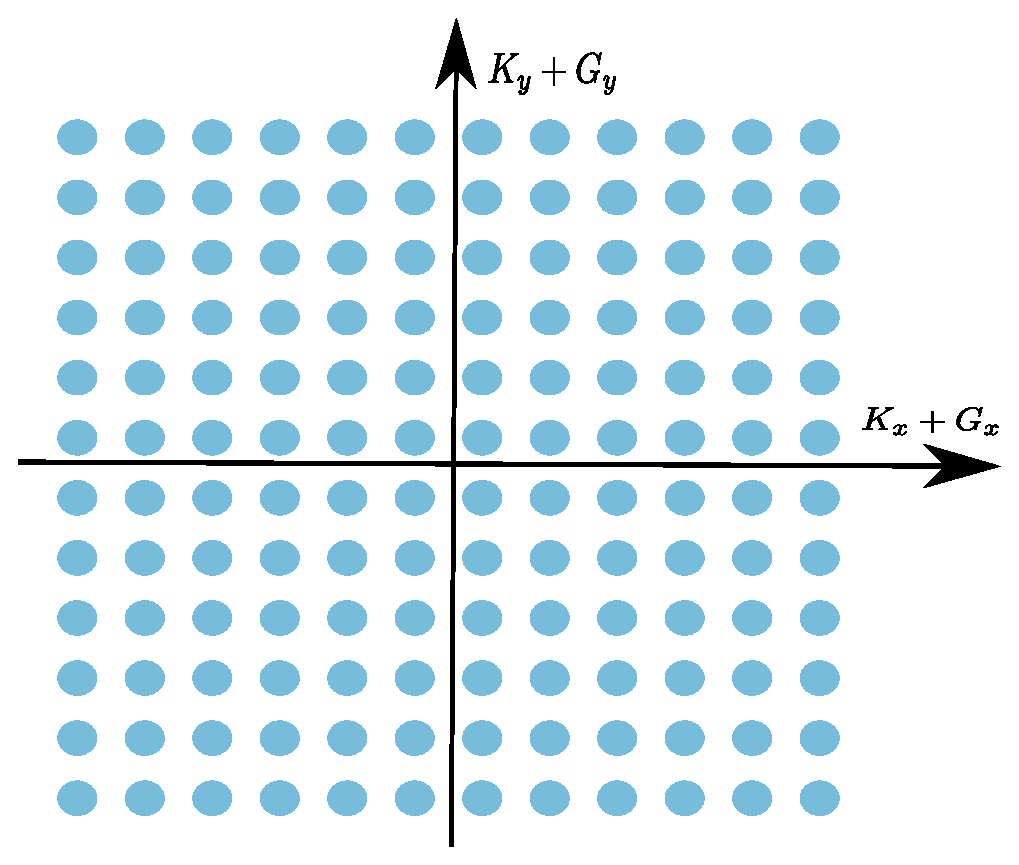
\epsfig{file=figuras/epacioKa.eps, width=5.0cm,height=5.0cm}
   		\label{fig:a-espacioK}
   	}
   \subfigure[]{
   	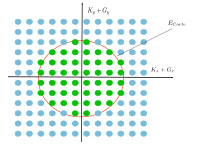
\epsfig{file=figuras/epacioKb.eps, width=5.0cm,height=5.0cm}
   	\label{fig:b-espacioK}
   }
   \caption[Mapeo espacio rec\'iproco]{en la figura \ref{fig:a-espacioK} se muestra el mapeo en el espacio rec\'iproco usando ondas planas. En la figura \ref{fig:b-espacioK} e muestra c\'omo  se trunca el espacio rec\'iproco por medio de la energ\'ia de corte $E_{corte}$\cite{MB-2015}.}
   \label{fig:espacioK}
   \end{figure}
   En la pr\'actica el n\'umero de ondas planas es limitado a una energ\'ia de corte $E_{corte}$ relacionada con la energ\'ia cin\'etica \cite{MB-2015}:
   \begin{equation}
   \int d \pmb{r}  \phi_{\pmb{k},\pmb{G}}^* (\pmb{r}) \left\{-\frac{1}{2} \nabla^2 \right\} \phi_{\pmb{k},\pmb{G}} (\pmb{r}) = \frac{1}{2} (\pmb{k}+ \pmb{G})^2 \le E_{corte}. \label{ec:Ecut}
   \end{equation}
   Esta energ\'ia determina el n\'umero de ondas planas que se usan en el c\'alculo y resultan al truncar el espacio rec\'iproco como se muestra en la figura \ref{fig:b-espacioK}, cuyo volumen es $\frac{4 \pi }{3} (2 E_{corte})^{3/2}$. Entonces el n\'umero de ondas planas por \'atomo $N_{PW}$ es \cite{PhysRevB.61.4576}:
   \begin{equation}
   N_{PW}\cdot N_{atomo} \approx \frac{4 \pi }{3} \frac{(2E_{corte})^{3/2}}{\Omega_{BZ}}. \label{ec:NumAtomoPW}
   \end{equation}
   Para muchos casos s\'olo se necesita una cantidad muy peque\~na de ondas planas tales como los \'atomos cuyos electrones de valencia pertenecen a los orbitales s y p si su comportamiento no se ve influido por los n\'ucleos. En el caso de que se tengan orbitales d se necesitar\'a una cantidad mayor de ondas planas debido a que estos estados est\'an mas localizados y por lo tanto se tienen que aumentar la energ\'ia de corte.
   \newline
   \par  La densidad y la energ\'ia total implican sumas en $\pmb{k}$ (o integrales sobre la primera zona de Brillouin ) y  se utilizan un n\'umero finito de  puntos en el espacio reciproco  resultando en un muestreo en la zona de Brillouin. El n\'umero de puntos depende de la dispersi\'on de las bandas ocupadas, donde t\'ipicamente se necesitan mas puntos $\pmb{k}$ para metales. anteriormente se tomaba en  cuenta  la simetr\'ia del sistema para obtener los puntos especiales $\pmb{k}^*$ en la zona irreducible de Brillouin; tales puntos eran suficientes para realizar estas sumas \cite{MB-2015}. Posteriormente se desarroll\'o   un m\'etodo para obtener estos puntos desarrollado por Monkhorst y Pack que realiza un muestreo con puntos $\pmb{k}$ equidistantes con pesos id\'enticos \cite{PhysRevB.13.5188}:
   \begin{equation}
   \pmb{k}_{n_1, n_2, n_3} = \sum_{i}^{3} \frac{2 n_i -N_i-1}{2N_i} \pmb{G}_i \label{ec:sampleMP}
   \end{equation}
   en donde $\pmb{G}_i $ son los vectores base del espacio rec\'iproco, $N_i$ es el n\'umero total de puntos en la direcci\'on $i$ y $n_i$ es el n]'umero de puntos \pmb{k} entre dos puntos en el espacio rec\'iproco conectados a trav\'es de  $\pmb{G}_i $.
    
   \section{C\'alculo de la Fuerza} \label{sec:Fuerza}
   \subsection{El teorema de Hellman-Feynman} \label{subsec:HellFey}
   Este teorema es de gran importancia en la f\'isica y el cual fue formulado Hellmann en 1937 \cite{Hellman-1937} y Feynman en 1939 \cite{PhysRev.56.340}, que consiste en obtener una expresi\'on  para la fuerza  que se ejerce en un n\'ucleo  y est\'a dado estrictamente en t\'erminos de la densidad electr\'onica independiente de la energ\'ia cin\'etica y de intercambio y correlaci\'on. Dicho  teorema tambi\'en es llamado  "Teorema de Fuerza" \cite{Martin-2004}. La fuerza puede ser escrita de la siguiente forma
   \begin{equation}
   \pmb{F}_I = - \frac{\partial E}{\partial \pmb{R}_I}. \label{ec:Fuerza}
   \end{equation} 
   Utilizando la expresi\'on general de la energ\'ia se obtiene la siguiente expresi\'on \cite{Martin-2004}
   \begin{equation}
   -\frac{\partial E}{\partial \pmb{R}_I} = - \left\langle \Psi \left| \frac{\partial \hat{H}}{\partial \pmb{R}_I} \right| \Psi \right\rangle- \left\langle \frac{\partial \Psi}{\partial \pmb{R}_I} \left| \hat{H} \right| \Psi \right\rangle - \left\langle \Psi \left| \hat{H} \right|  \frac{\partial \Psi}{\partial \pmb{R}_I} \right\rangle - \frac{\partial E_{II}}{\partial \pmb{R}_I}. \label{ec:expansionF}
   \end{equation}
   Utilizando el hecho de que se est\'a en el estado base se conoce que este es un extremo y por lo tanto los dos t\'erminos de en medio de la ecuaci\'on \ref{ec:expansionF} son cero. Por lo tanto la expresi\'on para la fuerza (omitiendo el spin) queda como \cite{MB-2015}:
   \begin{equation}
   \pmb{F}_I = -\frac{\partial E}{\partial \pmb{R}_I} = - \int d^3 r ~n(\pmb{r}) \frac{\partial V_{ext} (\pmb{r})}{\partial \pmb{R}_I}- \frac{\partial E_{II}}{\partial \pmb{R}_{II}}. \label{ec:FHFuerza} 
   \end{equation} 
   En el caso de que no se tenga un potencial local. no es posible expresar la fuerza en t\'erminos de la densidad electr\'onica pero a\'un es v\'alida la expresi\'on descrita anteriormente \cite{Martin-2004}
   \begin{equation}
   -\frac{\partial E}{\partial \pmb{R}_I} = - \left\langle \Psi \left| \frac{\partial \hat{H}}{\partial \pmb{R}_I} \right| \Psi \right\rangle - \frac{\partial E_{II}}{\partial \pmb{R}_I}. \label{ec:HFT}
   \end{equation}
   \subsection{C\'alculo auto consistente de fuerzas} \label{subsec:SConsFuerza}
   Es necesario redefinir la energ\'ia total $E_{tot} (\{\pmb{R}_I\})$ de un sistema con diferentes especies de n\'ucleos A,B, ..., los cuales est\'an fijos en las posiciones $\{\pmb{R}_I\} $ y en donde los electrones se mueven en un campo generado por los n\'ucleos $V_{ext} (\pmb{r})$. Las dos contribuciones mas importantes son la energ\'ia de los electrones en el estado base para cierta configuraci\'on $\{\pmb{R}_I\}$ de los n\'ucleos, la cual est\'a descrita por la energ\'ia de Kohn-Sham (ec. \ref{ec:funcHK} )  (omitiendo la constante de interacci\'on de los n\'ucleos y el spin) 
   \begin{multline}
   E_{KS} [n] = E_{V_{ext}} [n] = E_{KS} ([n],\{\pmb{R}_I\}) \\
   = T_{sp} [n] + \int d \pmb{r} V_{ext} n(\pmb{r}) + E_{Hartree} [n] + E_{XC} [n] \label{ec:KS_Fuerza}
   \end{multline}
   y la energ\'ia de la repulsi\'on de Coulomb  entre n\'ucleos ($E_{I I}$) (Sec. \ref{sec:introdft}, el \'ultimo t\'ermino es la ecuaci\'on \ref{ec:sh} ) se puede expresar como
   \begin{equation}
   	E_{II} = E_{nn} (\{\pmb{R}_I\}) = \frac{1}{2} \sum_{\substack{I,I' = 1 \\ (I \not = I')}}^ {N_n} Z_I Z_{I'} v(\pmb{R}_I - \pmb{R}_{I'}), \label{ec:IntII}
   \end{equation}
   en donde $ v(\pmb{R}_I - \pmb{R}_{I'})$ representa una interacci\'on de Coulomb. La energ\'ia total se puede representar como
   \begin{equation}
   E_{tot} (\{\pmb{R}_I\}) = E_{nn} (\{\pmb{R}_I\}) + E_{KS} ([n], \{\pmb{R}_I\}), \label{ec:EnTot2} 
   \end{equation}
   en donde  solo el potencial $V_{ext} (\pmb{r})$ depende expl\'icitamente de las coordenadas del n\'ucleo; as\'i mismo tampoco se consideran las vibraciones de red.
   \newline
   Para encontrar las posiciones $ \{\pmb{R}_I \}$ es necesario calcular la energ\'ia del estado base para la cierta configuraci\'on de $ \{\pmb{R}_I \}$ y para encontrar el m\'inimo global  de la energ\'ia total. Lejos del m\'inimo de la energ\'ia $E_{tot} (\{\pmb{R}_I\})$ existe una fuerza descrita por el teorema de Hellman-Feynman; en este caso se hace el cambio $\frac{\partial}{\partial \pmb{R}_I}  \rightarrow \nabla_{\pmb{R}_I}$ \cite{MB-2015}
   \begin{equation}
   \pmb{F}_I = - \nabla_{\pmb{R}_I} E_{tot} (\{\pmb{R}_I\}). \label{ec:Fuerza_Et}
   \end{equation}
   Para una dada composici\'on $N_A,N_B, ...$ y con cierta configuraci\'on $\{\pmb{R}_I\}$ la magnitud y la direcci\'on de una fuerza at\'omica provee informaci\'on acerca de que tan lejos est\'a cierto \'atomo de su posici\'on estable o metaestable, de tal forma que la geometr\'ia de equilibrio se determina cuando estas fuerzas netas son cero:
   \begin{equation}
   \pmb{F}_I |_{\{\pmb{R}_I\}= \{\pmb{R}_I^0\}} = 0 , ~~~~para~ todo~ I .\label{ec:fuerzaEq}
   \end{equation}
   La estructura \'optima $\{\pmb{R}_I^0\}$ de un s\'olido corresponde a un m\'inimo en la energ\'ia (ec. \ref{ec:EnTot2}). Este m\'inimo no es necesariamente el global y para encontrarlo se tienen que realizar m\'ultiples configuraciones y comparar la energ\'ia total. Usualmente se parte de una geometr\'ia inicial y se utiliza un segundo ciclo auto consistente para encontrar la geometr\'ia de equilibrio $\{\pmb{R}_I\}$. Este ciclo se muestra en la figura \ref{fig:esqFuerza}, el cual encapsula el ciclo auto consistente interno del c\'alculo de la energ\'ia, (fig. \ref{fig:esq}) \cite{MB-2015}.
   \begin{figure}[!hbt]
   	\centering
   	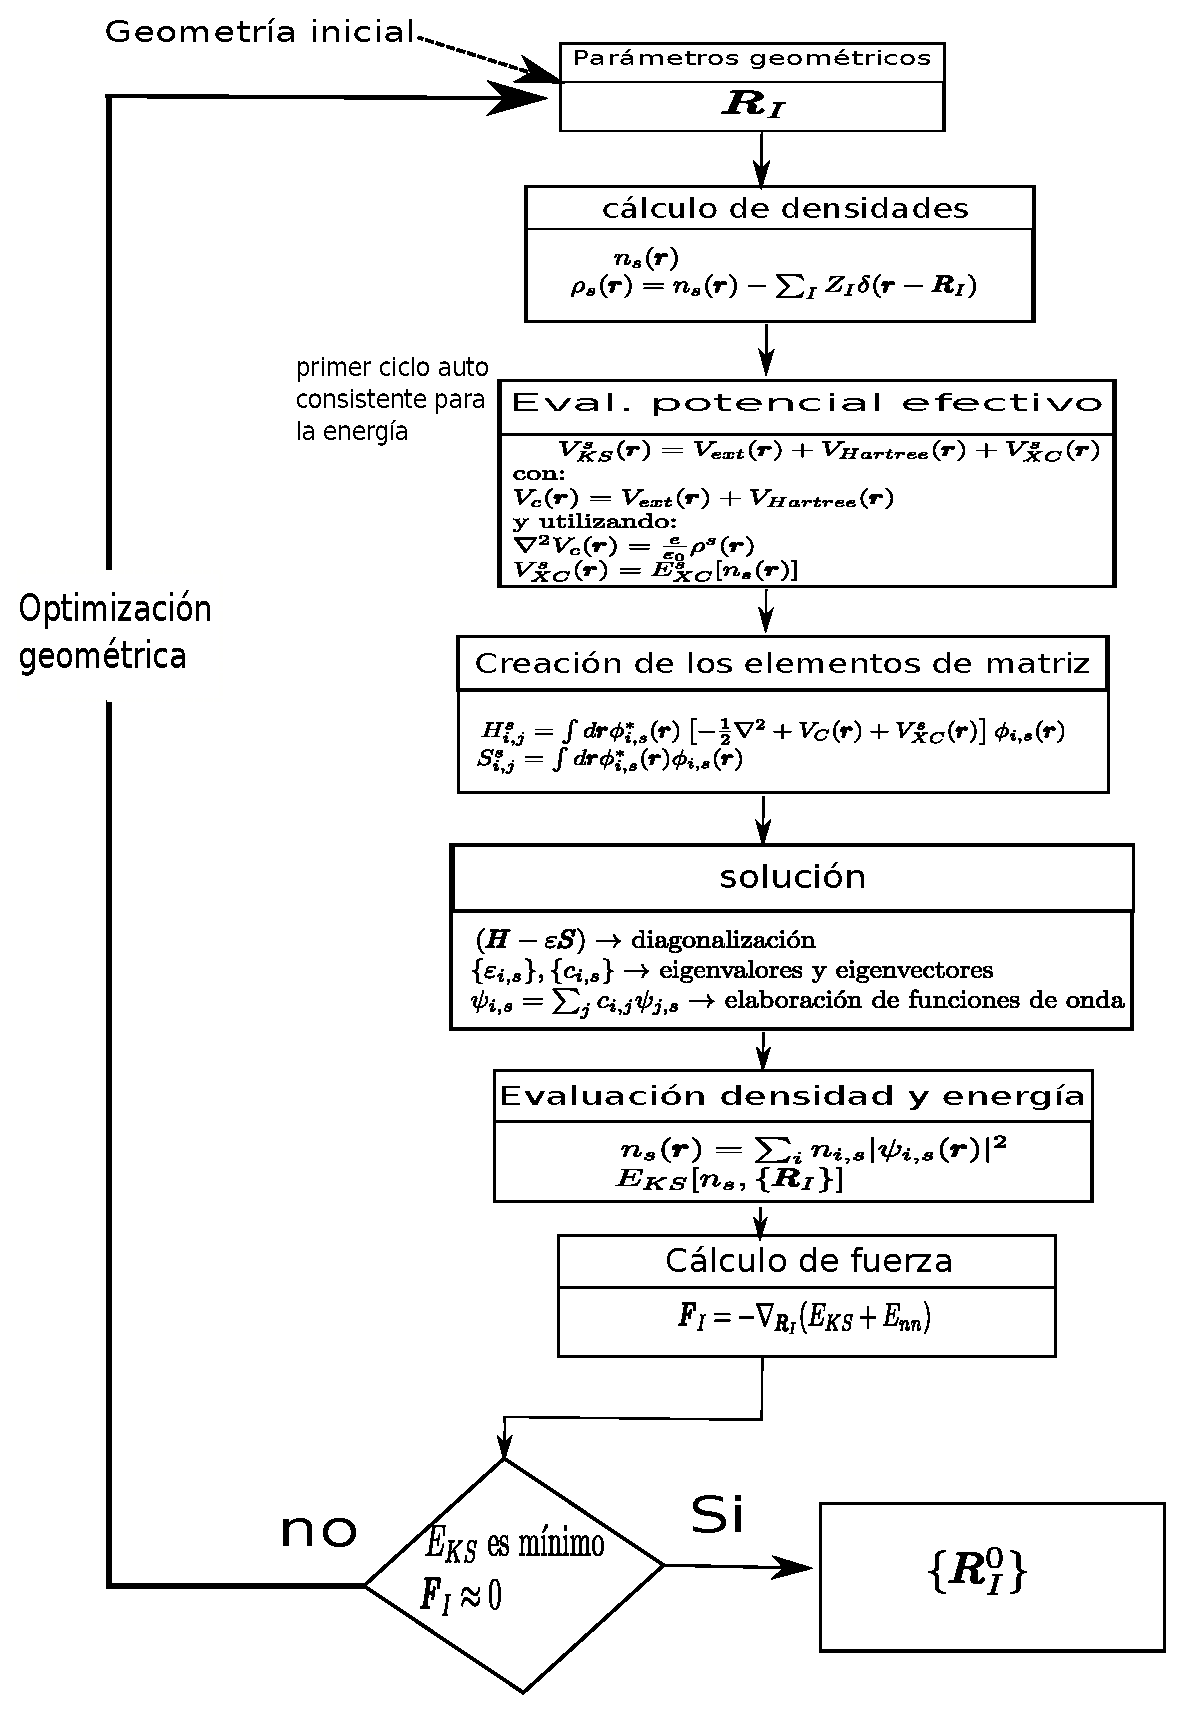
\epsfig{file=figuras/diagramaAuto2.eps, width=12.0cm,height=18.0cm}
   	\caption[C\'alculo auto consistente de fuerzas. ]{ciclo auto consistente para encontrar la geometr\'ia de equilibrio a partir de una geometr\'ia inicial $\{\pmb{R}_I^i\} $.}
   	\label{fig:esqFuerza}
   \end{figure}
   \newline
   Calculando las fuerzas de Hellman-Feynman utilizando la energ\'ia total (ec. \ref{ec:EnTot2}) se pueden obtener dos componentes \cite{doi:10.1080/00018738700101042}
   \begin{equation}
   	\pmb{F}_I = \pmb{F}_I^n + \pmb{F}_I^{el}, \label{ec:FuerzaDesc}
   \end{equation}
   en donde  la contribuci\'on debida a la repulsi\'on entre n\'ucleos es
   \begin{equation}
   \pmb{F}_I^n = \sum_{\substack{I,I' = 1 \\ (I \not = I')}}^{N_n} v(\pmb{R}_I - \pmb{R}_{I'}) \frac{\pmb{R}_I - \pmb{R}_{I'}}{|\pmb{R}_I - \pmb{R}_{I'}|^2}, 
   \end{equation}
   la cual es provocada por la energ\'ia de interacci\'on entre n\'ucleos (ec. \ref{ec:IntII}). Estudiando la contribuci\'on electr\'onica  (ec. \ref{ec:KS_Fuerza})se puede observar que s\'olo el potencial externo $V-{ext} (\pmb{r})$ depende expl\'icitamente de las posiciones nucleares $\{\pmb{R}_I\}$ y  la densidad $n(\pmb{r})$ depende impl\'icitamente de estas posiciones y acorde con el teorema de Hellman-Feynman (ec. \ref{ec:HFT}),  el \'ultimo t\'ermino en la ecuaci\'on \ref{ec:FuerzaDesc} se puede separar en dos t\'erminos \cite{doi:10.1080/00018738700101042}:
   \begin{equation}
   \pmb{F}_I^{el} = \pmb{F}_I^{el (1)} + \pmb{F}_I^{el (2)} \label{ec:descFel},
   \end{equation} 
   con
   \begin{equation}
   \pmb{F}_I^{el (1)} = - \int d \pmb{r} ~n(\pmb{r}) \nabla_{\pmb{R}_I} V_{ext} (\pmb{r}) \label{ec:Fel_1}
   \end{equation}
   y
   \begin{equation}
   \pmb{F}_I^{el(2)} = - \int d \pmb{r} \frac{\delta E_{KS} [n]}{\delta n(\pmb{r})} \nabla_{\pmb{R}_I} n(\pmb{r}). \label{ec:Fel_2} 
   \end{equation}
   De acuerdo con el segundo teorema de Hohenberg-Kohn, la ecuaci\'on \ref{ec:Fel_1} se hace cero cuando se logra el estado base del sistema. En tratamientos num\'ericos se pueden considerar fuerzas que se rigen con la ecuaci\'on \ref{ec:Fel_2}, las cuales se deben a inexactitudes num\'ericas en e c\'alculo de la densidad electr\'onica en el proceso observado en la figura \ref{fig:esqFuerza}. Usando la representaci\'on de la densidad electr\'onica en t\'erminos de los orbitales de Kohn-Sham $n(\pmb{r}) = \sum_i n_i |\psi_i (\pmb{r})|^2 $, la fuerza se puede como \cite{MB-2015}:
   \begin{equation}
   \pmb{F}_I^{el(2)} = -2 Re \sum_i n_i \int d \pmb{r} [\nabla_{\pmb{R}_I} \psi_i^* (\pmb{r})] \left[-\frac{1}{2} \nabla^2 + V_{KS} (\pmb{r}) - \varepsilon_i \right] \psi_i (\pmb{r}) \label{ec:F2scf}
   \end{equation}
   o
   \begin{eqnarray}
   \pmb{F}_I^{el(2)} = &-& 2 Re \sum_i n_i \int d \pmb{r} [\nabla_{\pmb{R}_I} \psi_i^* (\pmb{r})] \left[-\frac{1}{2} \nabla^2 + \tilde{V}_{KS} (\pmb{r}) -\varepsilon_i \right] \psi_i (\pmb{r}) \nonumber\\ 
   &-& \int d\pmb{r} [V_{KS} (\pmb{r})-\tilde{V}_{KS} (\pmb{r})] \nabla_{\pmb{R}_I} n(\pmb{r}). \label{ec:F2scf_2} 
   \end{eqnarray}
    El primer t\'ermino de la ecuaci\'on \ref{ec:F2scf_2} es cero si los cambios de las funciones de onda mantienen la orto-normalidad cuando un \'atomo se desplaza. Esto debe de cumplirse siempre cuando se utilizan  ondas planas como funciones base. 
      
   \section{Pseudopotenciales}\label{sec:pseudo}
   \subsection{Introducci\'on a los pseudopotenciales} \label{subsec:introPseudo}
   Es importante puntualizar que el uso de ondas planas solamente es una soluci\'on exacta si el potencial no var\'ia en el espacio y en el caso de que esta variaci\'on sea peque\~na  se puede tratar como una perturbaci\'on. Por lo general  el potencial externo $V_{ext}$ presenta variaciones considerables en las regiones cercanas a  las posiciones de los n\'ucleos $\pmb{R_I}$ \cite{Faustino-2014}; entonces la expansi\'on necesitar\'ia una cantidad mucho mayor de ondas planas para poder describir esta regi\'on del potencial. Es por esta raz\'on que es conveniente dividir en dos categor\'ias los electrones en el \'atomo: los electrones del n\'ucleo y los electrones de valencia. Los primeros son llamados así  debido a su cercan\'ia al n\'ucleo y no participan en la formaci\'on de enlaces qu\'imicos debido a que se encuentran fuertemente ligados a este. En cambio los electrones de valencia son los que determinan la mayor\'ia de las propiedades de los materiales debido a que son los que participan en la formaci\'on de  enlaces qu\'imicos. Estos electrones est\'an mas d\'ebilmente ligados al n\'ucleo por lo que es mas f\'acil describirlos con una expansi\'on de ondas planas.  Por lo tanto  se sustituye el efecto de los electrones de n\'ucleo con un pseudopotencial \cite{MB-2015}.
   \newline
   \par La idea del pseudopotencial se puede explicar distinguiendo entre estados de valencia($v$) y de n\'ucleo ($c$) y considerando un Hamiltoniano de un solo cuerpo $\hat{H} = \hat{T} + \hat{V}$  escribiendo la ecuaci\'on de Schr\"odinger con $\lambda= c,v$ \cite{PhysRev.116.287}
   \begin{equation*}
   \hat{H} | \psi_{\lambda} \rangle = \varepsilon_{\lambda} | \psi_{\lambda} \rangle. 
   \end{equation*}    
   Si se utiliza el m\'etodo OPW (Ortogonalized Plane Wave) \cite{PhysRev.57.1169}, se puede construir una pseudo funci\'on de onda $|\tilde{\psi}_v \rangle $ para los electrones de valencia
   \begin{equation}
   |\tilde{\psi}_v \rangle = | \psi_v \rangle + \sum_c a_{c,v} |\psi_c \rangle,
   \end{equation}
   en la cual se mezcla con los estados de n\'ucleo con $a_{c,v} = \langle \psi_c | \tilde{\psi}_v \rangle \not = 0$ y aun son ortogonales con los estados de n\'ucleo. Entonces las pseudo funciones de onda satisfacen la ecuaci\'on de  Schr\"odinger \cite{PhysRev.57.1169}
   \begin{equation}
   \left[\hat{H} + \sum_{c} (\varepsilon_v - \varepsilon_c) |\psi_c \rangle \langle \psi_c |\right] |\tilde{\psi}_v \rangle = \varepsilon_v | \tilde{\psi}_v \rangle .
   \end{equation}
   Para los eigenvalores $\{ \varepsilon_v \}$ y $ \{| \tilde{\psi}_v \rangle \}$ son correcciones suavizadas y correalcionan el pseudo Hamiltoniano $\hat{H}_{ps} = \hat{T} + \hat{V}_{ps}$ con el pseudopotencial
   $
   V_{ps}= V+ \sum_{c} (\varepsilon_v - \varepsilon_c) |\psi_c \rangle \langle \psi_c |,
   $
   el cual es dependiente de la energ\'ia.
   \newline
   \par En el caso de que se tenga un \'atomo aislado en $\pmb{R}_I = 0$ con simetr\'ia esf\'erica $V(\pmb{r}) = V(r)$ y con n\'umeros cu\'anticos $\lambda= n,l,m $, la funci\'on de onda se puede separar en \cite{MB-2015}
   \begin{equation}
   \psi_{nlm} (\pmb{r}) = R_{nl} (r) Y_{lm} (\theta, \phi) \label{ec:Psudofunc},
   \end{equation}
   donde $R_{nl}$ representa la parte radial y $Y_{lm} (\theta, \phi) $ son los  arm\'onicos esf\'ericos. Se puede esperar que el pseudopotencial act\'ue diferente en funciones de distinto momento angular.  La forma que tendr\'ia el pseudo potencial es \cite{PhysRev.57.1169} 
   \begin{equation}
   V_{ps} = \sum_{l=0}^{\infty} V_{ps}^l (r) \hat{P}_l \label{ec:PseudoV},
   \end{equation} 
   con el pseudopotencial parcial $V_{ps}^l (r) $ relacionado con el momento angular $l$, y el operador \cite{PhysRev.57.1169}
   \begin{equation}
   \hat{P}_l = \sum_{m=-l}^{l} |lm \rangle \langle lm | \label{ec:psudoProj},
   \end{equation}
   el cual opera en el espacio del $l$-\'esimo momento angular de tal forma que el pseudopotencial total (Ec. \ref{ec:PseudoV}) no es local.
   \subsection{Pseudopotenciales at\'omicos}
   Una propiedad importante de los pseudopotenciales es que puedan ser transferibles; es decir, que un pseudopotencial que se elabor\'o para cierto sistema se pueda utilizar en otro. La regi\'on del n\'ucleo tiene que estar "suavizada", es decir que se tiene que limitar la variaci\'on espacial. Para construir un pseudopotencial \textit{ab-initio} existen algunas reglas que ayudan a resolver el problema. Se comienza con la ecuaci\'on radial de Shr\"odinger (en unidades de Hartree) \cite{PhysRevB.26.4199}
   \begin{equation}
   \left\{-\frac{1}{2} \left[\frac{d^2}{dr^2} + \frac{l (l+1)}{2 r^2} \right]+ V(r)\right\} r R_l (\varepsilon,r) = \varepsilon r R_l (\varepsilon,r) \label{ec:ShRadial},
   \end{equation}  
   la cual es una ecuaci\'on de segundo orden y generalmente $\varepsilon$ se fija a $\varepsilon_l$. La soluci\'on se determina por la funci\'on radial $R_l (\varepsilon,r)  $ y su derivada $R'_l (\varepsilon,r)  $  y el potencial$V(r)$ es el potencial de Kohn-Sham (ec. \ref{ec:potKS}), como la suma del potencial de Coulomb de los n\'ucleos, el potencial de Hartree y el de intercambio y correlaci\'on, adem\'as de correcciones relativistas \cite{Martin-2004}(vistas en el ap\'endice \ref{corrRelApend}). 
   \newline
   \par Las reglas que se tienen que cumplir para construir los pseudopotenciales \textit{ab-initio} son \cite{PhysRevLett.43.1494, MB-2015}:
   \begin{enumerate}
   	\item Los pseudopotenciales reproducen los eigenvalores de energ\'ia $\tilde{\varepsilon}_l$ en acuerdo con aquellos $\varepsilon_l$ obtenidos por un c\'alculo con todos los electrones en los estados de valencia,
   	\begin{equation*}
   	\tilde{\varepsilon}_l = \varepsilon_l.
   	\end{equation*}  
   	\item A una distancia $r$ mayor al radio del n\'ucleo $r_{cl}$ la evaluaci\'on exacta es igual con la evaluaci\'on del pseudopotencial
   	\begin{equation*}
   	\tilde{R}_l (r) = R_l (r)~~~~~~~para~~~~~~r\ge r_{cl}.
   	\end{equation*}
   	\item \label{listNorm} En el caso $r < r_{cl}$, la parte pseudo-radial $\tilde{R}_l (r)$ no tiene grandes variaciones  y la norma tiene que ser la misma entre el calculo con todos los electrones y la pseudo funci\'on de onda. Esta regla es llamada la condici\'on de la conservaci\'on de la norma
   	\begin{equation*}
   	\int_{0}^{r_{cl}} dr~ r^2 |\tilde{R}_l (r)|^2 = \int_{0}^{r_{cl}} dr r^2 |R_l (r)|^2.
   	\end{equation*}
   	\item Adem\'as una propiedad importante para describir el esparcimiento de las ondas parciales, el cual se caracteriza por la fase de esparcimiento $\nu_l (\varepsilon)$ y cuya derivada de energ\'ia se relaciona con la derivada logar\'itmica \cite{Ziman-1972} 
   	\begin{equation}
   	D_l (\varepsilon, r) = \frac{1}{r} \frac{d \ln R_l (\varepsilon, r)}{d \ln r},
   	\end{equation}
   	se debe de cumplir lo siguiente en $r=r_{cl}$:
   	\begin{equation}
   	\tilde{D}_l (\varepsilon, r_{cl})= D_l (\varepsilon, r_{cl}) .
   	\end{equation}
   	
   \end{enumerate}
   La \'ultima regla indica que las propiedades de esparcimiento de dos \'atomos son similares en el rango de energ\'ia $\varepsilon$ de los electrones de valencia esto se relaciona con la identidad ($r \le r_{cl} $)
   \begin{equation}
   \frac{d}{d \varepsilon} D_l (\varepsilon, r) = - \frac{2 m }{\hbar} \frac{1}{r^2 R_l ^2 (\varepsilon, r)} \int_{0}^{r} dr' r^{'2} R_l ^2 (\varepsilon, r'), \label{ec:freidelSum} 
   \end{equation}
   que corresponde a la regla de suma de Freidel \cite{PhysRev.163.604}.
   \newline 
   \par El procedimiento para obtener el pseudopotencial  se inicia resolviendo la ecuaci\'on radial de Schr\"odinger para todos los electrones (ec. \ref{ec:ShRadial}) y el pseudopotencial puede ser construido con las reglas mencionadas anteriormente. De acuerdo a la regla \ref{listNorm} el pseudopotencial conserva la norma y existen distintos esquemas para construirlos.
   \newline
   \par En base a la ecuaci\'on de Schr\"odinger (ec. \ref{ec:ShRadial}) para las pseudo funciones de onda $\tilde{R}_l (r)$,  se construye  el pseudopotencial apantallado que es representado por la siguiente expresi\'on \cite{PhysRevB.26.4199}:
   \begin{equation}
   V_{ps}^{(sc)l} (r) = \varepsilon_l + \frac{\hbar}{2m} \left\{-\frac{l (l+1)}{r^2} + \frac{1}{r \tilde{R}_l (r)} \frac{d^2}{dr^2} [r \tilde{R}_l (r)]\right\} \label{ec:PSPot}.
   \end{equation}
    Los estados del n\'ucleo se utilizan  s\'olo a trav\'es del potencial auto consistente $V(r)$ y la expresi\'on \ref{ec:PSPot} claramente indica que el pseudopotencial es continuo y la funci\'on $\tilde{R}_l (r)$ se debe desvanecer como $r^l$ para $r \rightarrow 0$ para evitar la singularidad en el origen.
   \newline
   \par El pseudopotencial que act\'ua con los estados del momento angular $l$ se obtiene finalmente sustituyendo el efecto de interacci\'on con los electrones de valencia distribuidos acorde a sus pseudo funciones de onda \cite{PhysRevB.26.4199}
   \begin{equation}
   v_{ps}^l (r) = V_{ps}^{sc(l)} (r) - \int d^3 r \frac{1}{|\pmb{r}-\pmb{r'}|} \tilde{n}_v^{atomo} (\pmb{r'}) - V_{XC} (\pmb{r}; [\tilde{n}_v^{atomo} (\pmb{r'})]), \label{ec:pseudoSC1}
   \end{equation}   
   con densidad at\'omica esf\'erica:
   \begin{equation}
   \tilde{n}_v^{atomo} (\pmb{r})= \frac{1}{4 \pi} \sum_{l=0}^{l_{max}} \sum_{m=-l}^{l} |\tilde{R}_l (r)|^2. \label{ec:densAtomo}
   \end{equation}
   Si se substrae el efecto de los electrones de valencia se obtiene el pseudopotencial i\'onico (ec. \ref{ec:pseudoSC1}) el cual  es transferible.
   \newline
   \par De acuerdo con la ecuaci\'on \ref{ec:PSPot} cada momento angular $l$ tiene su propio pseudopotencial,  acorde con la ecuaci\'on \ref{ec:PseudoV} con el operador de proyecci\'on $\hat{P}_l$, los potenciales parciales se pueden combinar en un pseudopotencial total no local. En el l\'imite $r \rightarrow \infty$ se convierte en un potencial local $- Z^{val} e^2 / (4 \pi \varepsilon_0 r)$ con $Z^{val}$ igual al n\'umero de electrones de valencia en el \'atomo, debido a la condici\'on de cerradura del operador de proyecci\'on $\hat{P}_l$ requiere el mismo comportamiento para todo $l$ \cite{MB-2015}:
   \begin{equation}
   V_{ps}^l (r)= - \frac{Z^{val} e^2}{4 \pi \varepsilon_0 r} ~~~~para ~ r \rightarrow \infty.
   \end{equation}
   Como consecuencia es \'util descomponer $V_{ps}^l (r)$ en una contribuci\'on de largo alcance e independiente de $l$ y otra dependiente de $l$ y de corto alcance. La de largo alcance es local debido a $\sum_l \hat{P}_l =1$ y por esta raz\'on el pseudopotencial es semilocal debido a que son no locales en coordenadas $(\theta), (\phi)$ pero es local en la coordenada radial $r$ \cite{Martin-2004}.
   \newline
   \par Para generar un pseudopotencial que incluya la interacci\'on spin-\'orbita se realiza un c\'alculo relativista de todos los electrones con los  n\'umeros cu\'anticos $j=l+\frac{1}{2}$ y $j=l-\frac{1}{2}$ y es posible definir un potencial promedio y su diferencia como \cite{PhysRevB.26.4199, pickett_1989}
   \begin{eqnarray}
   V_{ps}^l (r) &=& \frac{1}{2 l +1} \left[l V_{ps}^{l-\frac{1}{2}} (r) + (l+1) V_{ps}^{l+\frac{1}{2}} (r)  \right], \\
   \Delta V_{ps}^l (r) &=& \frac{1}{2 l +1} \left[V_{ps}^{l+\frac{1}{2}} (r) -  V_{ps}^{l-\frac{1}{2}} (r)  \right].
   \end{eqnarray} 
   Estas ecuaciones ofrecen una contribuci\'on adicional a la ecuaci\'on  \ref{ec:PSPot}, la cual se puede representar como \cite{PhysRevB.34.2920, PhysRevB.64.073106}:
   \begin{equation}
   \Delta V_{ps}^{so} = \sum_{l,m} |lm \rangle \Delta V_{ps}^{l} (r)  \pmb{l} \cdot \pmb{s} \langle lm| \label{ec:psudoSO},
   \end{equation}
   con el operador de momento angular $\pmb{l} $ y el operador de spin $\pmb{s}$.
   \subsection{M\'etodo PAW}\label{subsec:PAW}
   El m\'etodo del proyector de ondas aumentadas (PAW, Projector Augmented Wave) \cite{PhysRevB.59.1758, PhysRevB.50.17953} es una aproximaci\'on general para la soluci\'on del problema de DFT que reformula el m\'etodo OPW descrito en la secci\'on \ref{subsec:introPseudo}. Este m\'etodo introduce proyectores en la soluci\'on del pseudopotencial.  El m\'etodo consiste en tomar una funci\'on "suave" $~\tilde{\psi}_i^v (\pmb{r})$ y una transformaci\'on lineal  $\psi^v = \mathcal{T} \tilde{\psi}^v  $ tales que relacionen el conjunto de las funciones de onda $\psi^v $ con la pseudo funciones de onda $ \tilde{\psi}^v$ y se sume que es unitaria excepto en la regi\'on definida por una esfera centrada en el n\'ucleo $\mathcal{T} = \pmb{1}+ \pmb{T}_0$. A continuaci\'on  se omite por motivos de simplicidad, el exponente $v$ y la etiquetas $j$ \cite{PhysRevB.59.1758}.  Utilizando la notaci\'on de Dirac se puede escribir la siguiente ecuaci\'on para la pseudo funci\'on de onda \cite{PhysRevB.59.1758, Martin-2004}:
   \begin{equation}
   | \tilde{\psi} \rangle = \sum_m c_m | \tilde{\psi}_m \rangle \label{ec:DiracPseudo},
   \end{equation}
   y la funci\'on de onda
   \begin{equation}
   |\psi \rangle = \mathcal{T} |\tilde{\psi} \rangle = \sum_m c_m | \psi_m \rangle. \label{ec:DiracAllE}
   \end{equation}
   Utilizando las ecuaciones \ref{ec:DiracPseudo} y \ref{ec:DiracAllE} se puede escribir  la funci\'on de onda en todo el espacio  \cite{PhysRevB.59.1758}
   \begin{equation}
   | \psi \rangle = |\tilde{\psi} \rangle + \sum_m c_m \left\{|\psi_m \rangle - |\tilde{\psi}_m \rangle \right\}. \label{ec:DiracFunc}
   \end{equation}
   Si la transformaci\'on $\mathcal{T}$ es lineal, entonces se tiene que cumplir con \cite{doi:10.1063/1.2338035}:
   \begin{equation}
   	c_m = \langle \tilde{p}_m | \tilde{\psi} \rangle,  \label{ec:condProj}
   \end{equation}
   para alg\'un proyector $\tilde{p}$ y cumple con la condici\'on de ortogonalidad
   \begin{equation}
   \langle \tilde{p}_m | \tilde{\psi}_{m'} \rangle = \delta_{m,m'}. \label{ec:orotoDirac}
   \end{equation}
   Para los pseudopotenciales existen muchas opciones para los proyectores y en este m\'etodo la transformaci\'on $\mathcal{T}$ a\'un contiene la funci\'on de onda de todos los electrones \cite{doi:10.1063/1.2338035}
   \begin{equation}
   \mathcal{T} = \pmb{1} + \sum_m \left\{ |\psi_m\rangle - |\tilde{\psi}_m \rangle \right\} \langle \tilde{p}_m |. \label{ec:ProjectorPAW}
   \end{equation}
   Esta expresi\'on aplica tanto para los electrones de valencia como para los electrones de n\'ucleo.
   \newline
   \par La forma general de las ecuaciones PAW se pueden obtener en funci\'on de la transformaci\'on de la Ec. \ref{ec:ProjectorPAW} para cualquier operador $\hat{A}$. Cuando se consideran todos los electrones se puede obtener un nuevo operador $\tilde{A}$ que se proyecte en la parte suave de las funciones de onda \cite{PhysRevB.50.17953}:
   \begin{equation}
   \tilde{A}= \mathcal{T} ^{\dagger} \hat{A} \mathcal{T} = \hat{A} + \sum_{m,m'} |\tilde{p}_m \rangle \left\{\langle \psi_m | \hat{A} | \psi_{m'} \rangle - \langle \tilde{\psi}_m | \hat{A} | \tilde{\psi}_{m'} \rangle \right\} \langle \hat{p}_{m'}| \label{ec:operadorPseudo}.
   \end{equation}
   Adem\'as se puede sumar a la ecuaci\'on \ref{ec:operadorPseudo} un operador de la forma
   \begin{equation}
   \hat{B}-\sum_{m,m'} |\tilde{p}_m \rangle \langle \tilde{\psi}_m | \hat{B} | \tilde{\psi}_{m'} \rangle \langle \tilde{p}_{m'}| 
   \end{equation}
   que no cambia los valores de expectaci\'on. La expresi\'on para la densidad en la teor\'ia PAW se puede expresar como \cite{PhysRevB.50.17953}:
   \begin{equation}
   n(\pmb{r}) = \tilde{n} (\pmb{r}) + n^1 (\pmb{r}) - \tilde{n}^1 (\pmb{r}), \label{ec:densidadPAW}
   \end{equation}
   la cual se puede escribir en t\'erminos de los eigenestados $i$ y con las ocupaciones $n_i$ como
   \begin{equation}
   \tilde{n} (\pmb{r}) = \sum_i n_i |\tilde{\psi}_i (\pmb{r})|^2, \label{ec:densPW}
   \end{equation}
   \begin{equation}
   n^1 (\pmb{r}) = \sum_i n_i \sum_{m,m'} \langle \tilde{\psi}_i | \tilde{\psi}_m \rangle \psi_m ^* (\pmb{r}) \psi_{m'} (\pmb{r}) \langle \tilde{\psi}_{m'} | \tilde{\psi}_i \rangle \label{ec:n1} 
   \end{equation}
   y
   \begin{equation}
   \tilde{n}^1 (\pmb{r}) = \sum_i n_i \sum_{m,m'} \langle \tilde{\psi}_i | \tilde{\psi}_m \rangle \tilde{\psi}_m ^* (\pmb{r}) \tilde{\psi}_{m'} (\pmb{r}) \langle \tilde{\psi}_{m'} | \tilde{\psi}_i \rangle. \label{ec:tn1}
   \end{equation}
   Estos dos t\'erminos est\'an localizados en cada \'atomo y las integrales pueden ser evaluadas  en coordenadas esf\'ericas.  
    \endinput
		\chapter{Efecto Kerr magneto-\'optico} \label{cap:Kerr}
\section{Introducci\'on al efecto Kerr magneto-\'optico} \label{Kerr:sec:Intr}
Una manera de estudiar las propiedades magn\'eticas de los materiales es haciendo uso de los efectos magneto-\'opticos, los cuales surgen como resultado de la interacci\'on entre la luz y la materia que es sujeta a un campo magn\'etico y que en el caso de materiales que tengan cierto orden magn\'etico, tales como los materiales ferromagn\'eticos, se siguen observando estos fen\'omenos en el caso de que no se apliquen campos magn\'eticos externos. Dichos fen\'omenos provienen de la separaci\'on de niveles de energ\'ia inducidos por la aplicaci\'on de un campo magn\'etico externo; es decir proviene del efecto Zeeman y lo cual provoca que cambie el espectro del coeficiente de  absorbci\'on y tiende a la aparici\'on o a la variaci\'on de la anisotropía magn\'etica. La anisotrop\'ia de un medio magnetizado se puede observar en la reflexi\'on de la luz en la superficie, el cual es el llamado efecto Kerr magneto-\'optico, que fue descubierto por  John Kerr en 1888 observando el cambio de polarizaci\'on  lineal a eliptica provocado por la reflexi\'on de la luz en un electroim\'an pulido \cite{Kerr_1888}.  
\newline
\par En la espectroscopia de efecto Kerr magneto-\'optico generalmente se distingue entre la polarizaci\'on lineal incidente entre $s$ y $p$, en las cuales el campo el\'ectrico est\'a normal ($s$) o paralelo ($p$) al plano de incidencia y estas propiedades magneto-\'opticas dependen de las polarizaciones $s$ y $p$ \cite{mo_2004}.
\newline
\par Se pueden caracterizar tres tipos de  efecto Kerr dependiendo de la orientaci\'on del vector de magnetizaci\'on con respecto a la superficie y al plano de incidencia del haz: polar, longitudinal y transversal, los cuales se observan en la figura \ref{Kerr:fig:Conf}. La configuraci\'on polar (fig. \ref{Kerr:fig:pol}) se tiene cuando el vector de magnetizaci\'on se orienta en la direcci\'on perpendicular a la superficie del material y paralelamente al plano de incidencia. La geometr\'ia longitudinal (fig. \ref{Kerr:fig:long}) se obtiene cuando se orienta el vector de magnetizaci\'on paralelamente a la superficie del material y al plano de incidencia y la configuraci\'on transversal se da cuando se orienta perpendicularmente al plano de incidencia y  paralelamente a la superficie.  La influencia de la magnetizaci\'on el las configuraciones polar  y longitudinal provoca la rotaci\'on del plano de polarizaci\'on y la aparici\'on de  la elipticidad de la luz reflejada. En cambio en la configuraci\'on transversal, solo se observa el cambio de la intensidad y la fase del haz incidente \cite{mo_2004}.
\begin{figure}[!hbt]
	\centering
	\subfigure[polar]{
		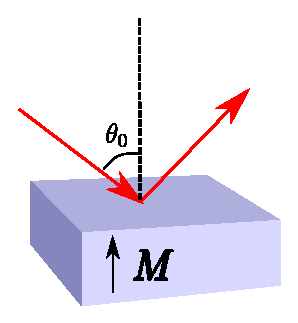
\epsfig{file=figKerr/pol/pol.eps, width=5.0cm,height=5.0cm}
		\label{Kerr:fig:pol}
	}
    \subfigure[longitudinal]{
    	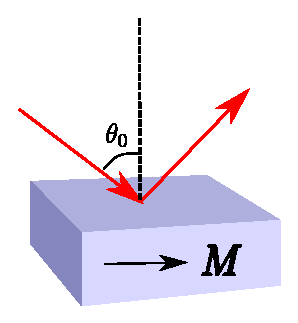
\epsfig{file=figKerr/pol/long.eps, width=5.0cm,height=5.0cm}
    	\label{Kerr:fig:long}
    }
    \subfigure[transversal]{
    	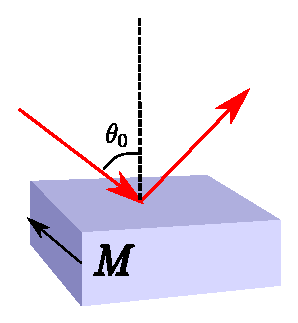
\epsfig{file=figKerr/pol/trans.eps, width=5.0cm,height=5.0cm}
    	\label{Kerr:fig:trans}
    }
   \caption[Configuraciones de Efecto Kerr magneto-\'optico.]{Diferentes configuraciones del efecto Kerr magneto-\'optico}
   \label{Kerr:fig:Conf}
\end{figure}
\newline
La constante de diel\'ectrica $\hat{\epsilon}$ se puede escribir de la siguiente forma asumiendo que las componentes $\epsilon_{xx} \approx \epsilon_{zz}$ \cite{You_1996}:
\begin{equation}
\hat{\epsilon}= \epsilon_{xx}
\begin{pmatrix}
1         & -i Q_1 m_z & i Q_2 m_y \\
i Q_1 m_z & 1          &  i Q_3 m_x\\
-i Q_2 m_y&-i Q_3 m_x  & 1
\end{pmatrix}
\label{Kerr:ec:consDiel},
\end{equation}
en donde $m_{x,y,z}$ son los cosenos directores del vector de magnetizaci\'on y
\begin{equation*}
\left(Q_1, Q_2, Q_3\right)= \left(i \frac{\epsilon_{xy}}{\epsilon_{xx}},-i \frac{\epsilon_{xz}}{\epsilon_{xx}}, -i \frac{\epsilon_{yz}}{\epsilon_{xx}} \right)
\end{equation*}
son las constantes giromagn\'eticas del material \cite{mo_2004,You_1996}. Es importante notar que las componenetes del tensor diel\'ectrico $\hat{\epsilon}_{\alpha, \beta}$ tienen componentes reales e imaginarias $\hat{\epsilon}_{\alpha, \beta} = \epsilon_{\alpha, \beta}^{(1)} +i\epsilon_{\alpha, \beta}^{(2)} $, donde $\alpha,\beta \equiv x,y,z$, $\epsilon_{xx}= (n+k)^2$,  siendo $n$ y $k$ el \'indice de refracci\'on y de extinci\'on respectivamente. El tensor diel\'ectrico se relaciona con el de la conductividad $\hat{\sigma}_{\alpha, \beta} = \sigma_{\alpha, \beta}^{(1)} +i\sigma_{\alpha, \beta}^{(2)} $ de la siguiente forma:
\begin{equation}
\hat{\epsilon}_{\alpha,\beta}(\omega)= \delta_{\alpha,\beta}+ \frac{4 \pi i}{\omega}\hat{\sigma}_{\alpha,\beta}(\omega) \label{Kerr:ec:relES}.
\end{equation}
De igual manera se puede definir el coeficiente de refracci\'on complejo $\hat{N}(\omega)$:
\begin{equation}
\hat{N} (\omega) \equiv \sqrt{\hat{\epsilon} (\omega)} = n(\omega) + k(\omega). \label{Kerr:ec:N}
\end{equation}  
Resolviendo las ecuaciones de Maxwell utilizando el tensor diel\'ectrico (ec. \ref{Kerr:ec:consDiel}) se encuentra que  la matriz de reflexi\'on de Fresnel, la cual es utilizada en el an\'alisis de Jones del ap\'endice \ref{Jones:App}, se puede escribir como:
\begin{equation}
R=
\begin{pmatrix}
\tilde{r}_{pp}  &  \tilde{r}_{ps} \\
\tilde{r}_{sp}  &  \tilde{r}_{ss}
\end{pmatrix}
\label{Kerr:ec:ref},
\end{equation}
en donde $\tilde{r}_{i,j}$ es la raz\'on entre el campo eléctrico incidente $j$ y el campo reflejado $i$, cuyas expresiones se pueden encontrar el art\'iculo de Chun-Yeol You \cite{You_1996}. Los efectos magneto-\'opticos se pueden definir en funci\'on de estos par\'ametros escribiendo el \'angulo Kerr complejo \cite{You_1996}:
\begin{subequations}
	\begin{gather}
	\Theta_K ^p = \theta_K^p + i \eta_K^p \equiv \frac{\tilde{r}_{sp}}{\tilde{r}_{pp}}, \label{Kerr:ec:AngKp} \\
	\Theta_K ^s = \theta_K^s + i \eta_K^s \equiv \frac{\tilde{r}_{ps}}{\tilde{r}_{ss}}, \label{Kerr:ec:AngKs}
	\end{gather}
\end{subequations}
en donde $\theta_K$ es el \'angulo de rotaci\'on de la polarizaci\'on  y $\eta_K$ es la elipticidad de el haz de luz, que ambas  son utilizadas para obtener las ecuaciones para el efecto Kerr en sus tres configuraciones.
\section{Efecto Kerr longitudinal} \label{Kerr:sec:long}
En el caso de la configuraci\'on longitudinal se asume que $m_x = m_z =0$ y $m_z =1$ y por lo tanto el tensor diel\'ectrico se puede escribir como:
\begin{equation}
\hat{\epsilon}= 
\begin{pmatrix}
\epsilon_{xx} & 0           &\epsilon_{xz} \\
0             &\epsilon_{xx}& 0            \\
-\epsilon_{xz}&0            &\epsilon_{xx} 
\end{pmatrix}.
\label{Kerr:ec:tensDielL}
\end{equation}
La ecuaci\'on para el \'angulo Kerr complejo con la configuraci\'on longitudinal se encuentra utilizando las ecuaciones para el caso general \cite{mo_2004}:
\begin{equation}
\Theta_K^{s,p} =-\frac{\hat{\epsilon}_{xz} \sin (\theta_0) \left(\sqrt{\hat{\epsilon}_{xx}-\sin^2(\theta_0) } \pm \sin(\theta_0) \tan(\theta_0)\right)}{(\hat{\epsilon}_{xx}-1) (\hat{\epsilon}_{xx}-\tan^2 (\theta_0))\sqrt{\hat{\epsilon}_{xx}-\sin^2(\theta_0) }}, \label{Kerr:ec:AngCompL}
\end{equation}
en donde $\theta_0$ es el \'angulo de incidencia del haz mostrado en la figura \ref{Kerr:fig:long} y los signos $(+)$  y $(-)$ corresponde a la polarizaci\'on $s$ y $p$, respectivamente. En el caso de la aproximaci\'on  $\epsilon_{xx} \approx \epsilon_{zz}$ ya no sea v\'alida se usa la siguiente expresi\'on \cite{mo_2004}:
\begin{equation}
\Theta_K^{s,p} = - \frac{2 \hat{\epsilon}_{xz} \sin (\theta_0) \cos(\theta_0) \sqrt{\hat{\epsilon}_{xx}}}{D}, \label{Kerr:ec:AngSApr}
\end{equation}
con
\begin{multline*}
D= \left(\sqrt{\hat{\epsilon}_{xx}(\hat{\epsilon}_{zz}- \sin^2(\theta_0))}+\sqrt{\hat{\epsilon}_{zz}(\hat{\epsilon}_{xx}- \sin^2(\theta_0))} \right) \times \\
\left(\sqrt{\hat{\epsilon}_{xx}- \sin^2(\theta_0)} \pm \cos(\theta_0) \right) \left(\sqrt{\hat{\epsilon}_{xx} \hat{\epsilon}_{zz}} \cos(\theta_0)\mp \sqrt{\hat{\epsilon}_{zz}- \sin^2(\theta_0)}\right).
\end{multline*}
La ecuaci\'on \ref{Kerr:ec:AngSApr} y su aproximaci\'on (ec. \ref{Kerr:ec:AngCompL}), son las expresiones fundamentales para explicar la espectroscopia del efecto Kerr magneto-\'optico.
\endinput 
		\chapter{M\'etodos Computacionales y Experimentales} \label{cap:Metodos}
\section{M\'etodos computacionales} \label{Met:sec:mcomp}
Para poder implementar la teor\'ia descrita en el cap\'itulo \ref{cap:DFT} se utiliza el software libre Quantum-Espresso \cite{Giannozzi_2009,Giannozzi_2017}, el cual permite realizar c\'alculos de propiedades de materiales utilizando t\'ecnicas de primeros principios. Para poderlo emplear  es necesario realizar un modelo con la estructura at\'omica del material en cuesti\'on y  por este motivo es necesario crear una supercelda cuya elaboraci\'on se explica en la subsecci\'on \ref{Met:subsec:supercelda} y los detalles computacionales se explican en la secci\'on \ref{Met:subsec:detcomp}.
\subsection{Supercelda}  \label{Met:subsec:supercelda}
Para realizar una supercelda se  parte de la  celda unitaria del cristal que se puede obtener de bases de datos  de c\'alculos de primeros principios \cite{Jain2013}. Las superceldas son creadas utilizando el software VESTA \cite{Momma:db5098} y para visualizar dichas estructuras y las distribuciones de carga y magnetizaci\'on se utiliza XcrySDen \cite{kokalj_1999}.  En el presente trabajo se quieren estudiar las propiedades magn\'eticas inducidas por defectos y deformaciones en los siguientes materiales: Disulfuro de Vanadio $VS_2  \cite{osti_1308135} $, Diseleniuro de Vanadio$~VSe_2 \cite{osti_1284665}$, Disulfuro de Platino$~PtS_2 \cite{osti_1292393}$ y Diseleniuro de Platino $PtSe_2 \cite{osti_1187595}$, en primer lugar se crearon las superceldas  unitarias que son utilizadas para estudiar las propiedades magn\'eticas de los materiales sin vacancias. Para elaborarlas simplemente se desplaza la celda unitaria  para colocar el metal de transici\'on entre dos calcogenuros y posteriormente se la agrega una capa de vac\'io. En la figura \ref{Met:fig:SupU} se muestra esta estructura. 
\begin{figure}[hbt!]
	\centering
	\subfigure[]{
		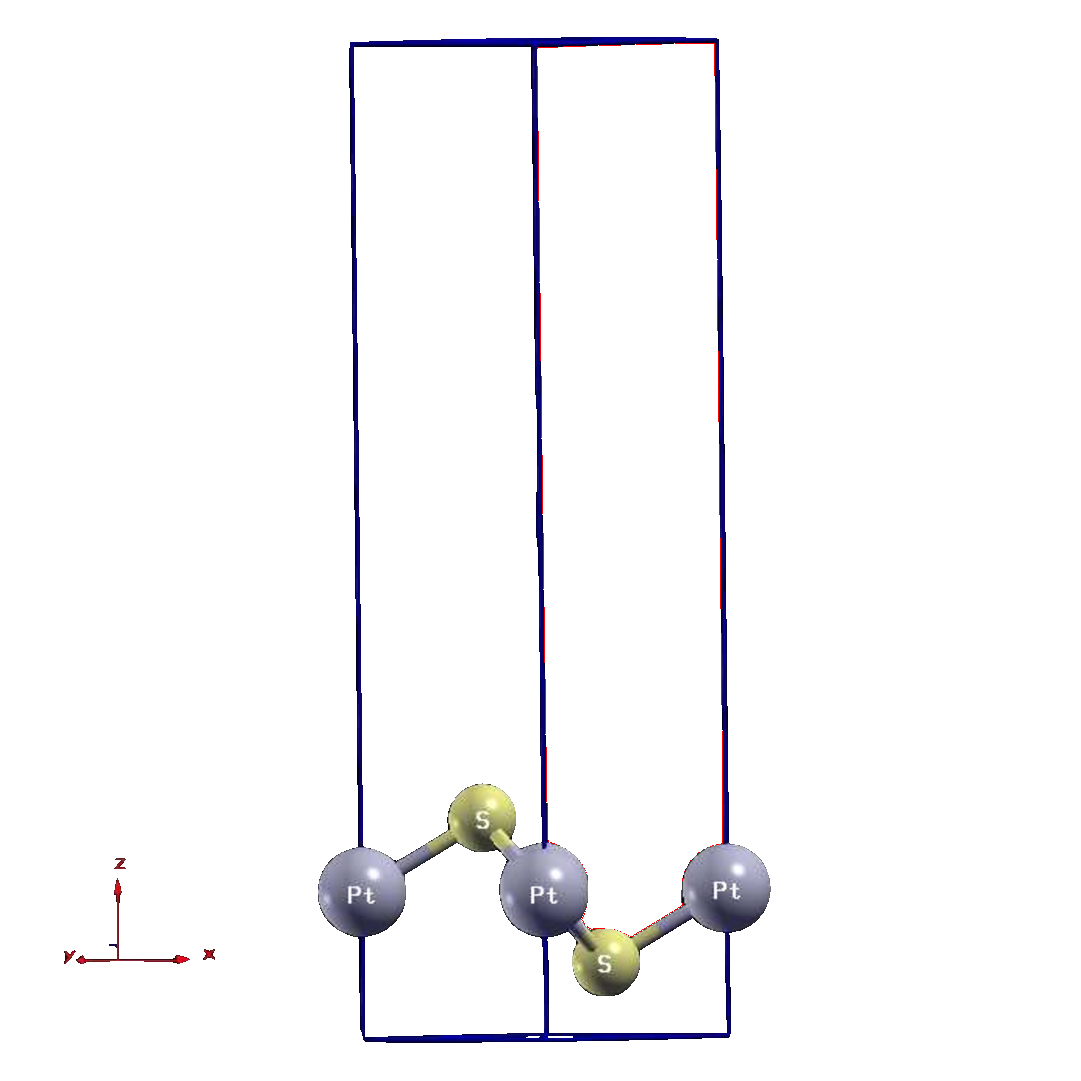
\epsfig{file=figMet/superceldaLado.eps, width=6.0cm,height=6.0cm}
		\label{Met:fig:supUcanto}
	}
    \subfigure[]{
    	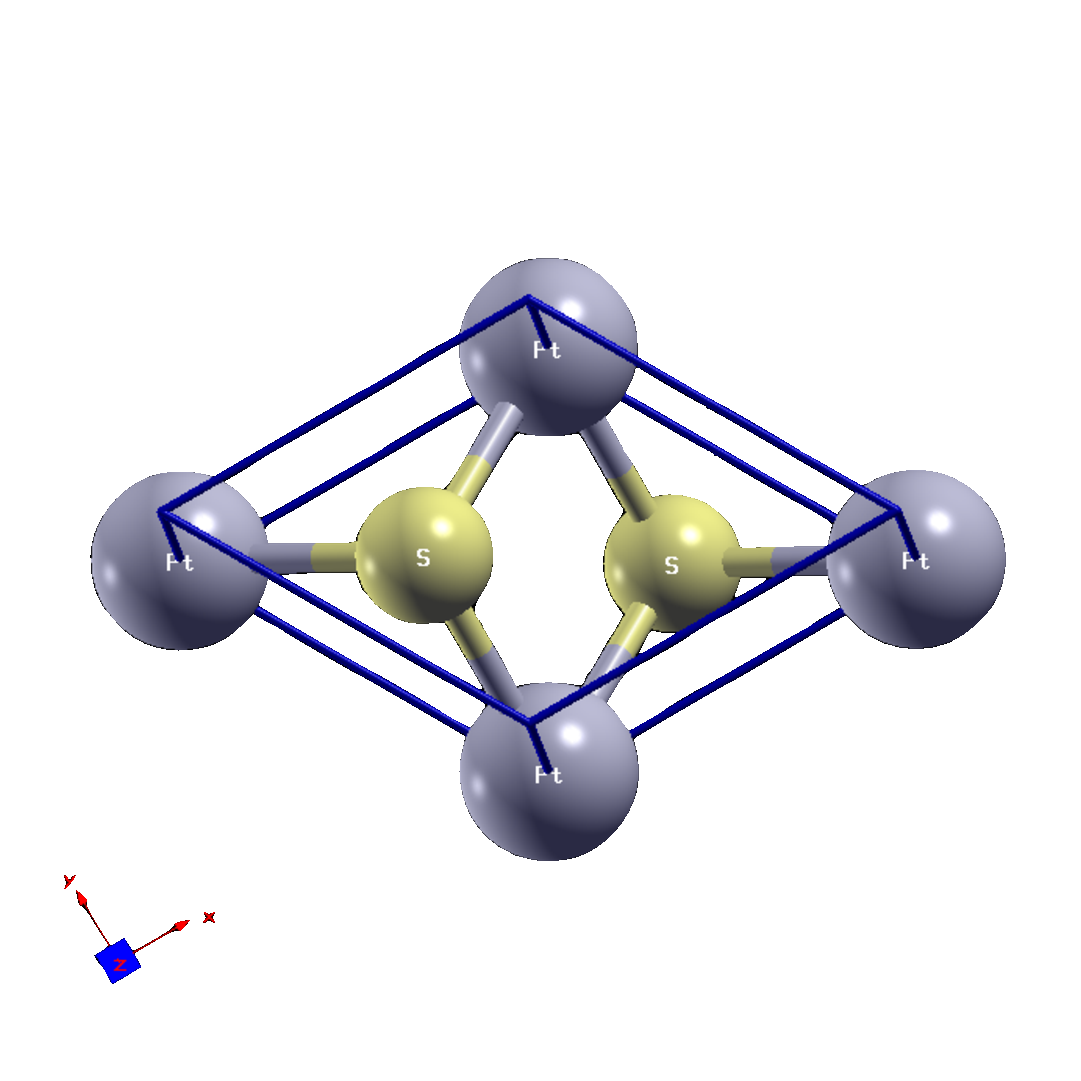
\epsfig{file=figMet/superceldaarriba.eps, width=6.0cm,height=6.0cm}
    	\label{Met:fig:supUarriba}
    }
    \caption[Supercelda de los materiales estudiados]{ Visualizaci\'on de la supercelda de $PtS_2$ vista de canto (\ref{Met:fig:supUcanto}) y desde arriba (\ref{Met:fig:supUarriba}). Por motivos visuales se agregan tres \'atomos de Platino.}
    \label{Met:fig:SupU}
\end{figure}   
\newline
\par  Para estudiar la vacancias del metal de transición, primeramente se crea una supercelda con cuatro celdas unitarias de tal forma que se tienen 12 \'atomos, cuatro metales de transici\'on y ocho calc\'ogenos y  se le agrega una capa de vac\'io. Posteriormente  se elimina un \'atomo del metal para crear la vacancia. En la figura \ref{Met:fig:SupV} se muestran los \'atomos en las posiciones en las que la energ\'ia y fuerza son m\'inimas en una supercelda con la vacancia de Platino; es decir est\'an optimizados (sec. \ref{sec:Fuerza}).
\begin{figure}[hbt!]
	\centering
	\subfigure[]{
		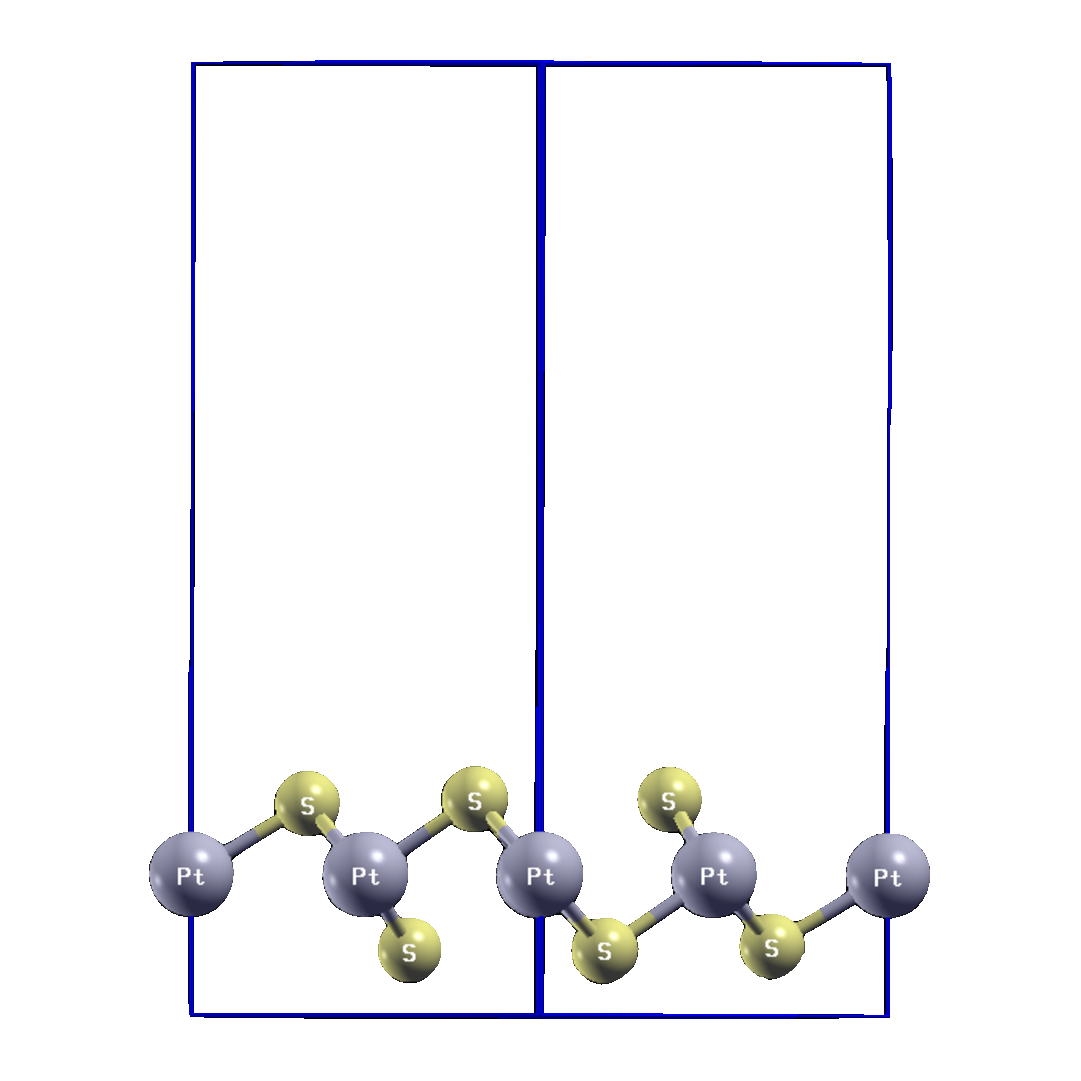
\epsfig{file=figMet/superceldaVacanciaLado.eps, width=7.0cm,height=7.0cm}
		\label{Met:fig:supVcanto}
	}
	\subfigure[]{
		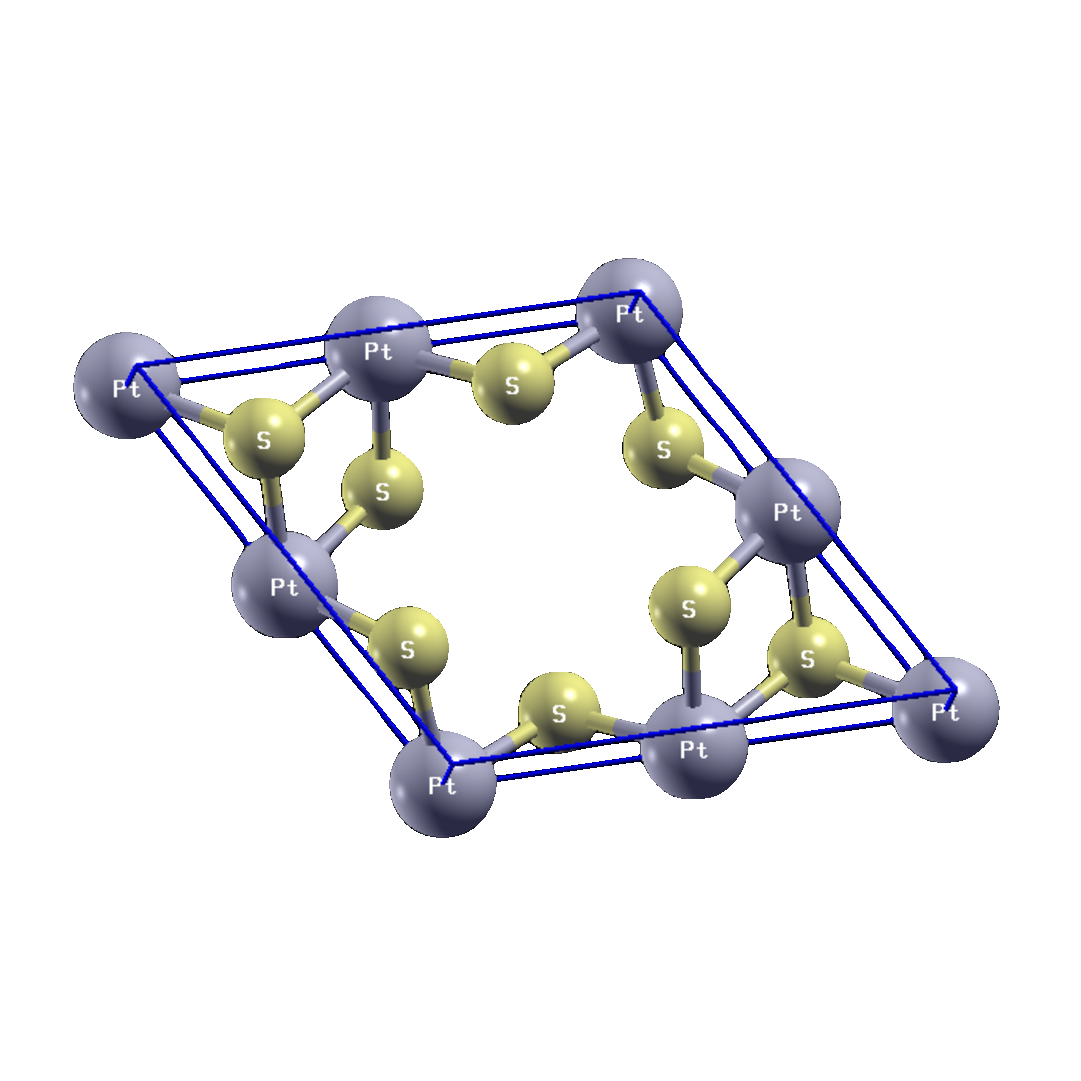
\epsfig{file=figMet/superceldaVacanciaArriba.eps, width=7.0cm,height=7.0cm}
		\label{Met:fig:supVarriba}
	}
	\caption[Estructura de la supercelda.]{ Visualizaci\'on de la supercelda de $PtS_2$  con vacancia de Pt en el software XcrySDen vista de canto (\ref{Met:fig:supVcanto}) y desde arriba (\ref{Met:fig:supVarriba}). Por motivos visuales se agregan tres \'atomos de Platino.}
	\label{Met:fig:SupV}
\end{figure}
\subsection{Detalles computacionales} \label{Met:subsec:detcomp}
  Se utiliz\'o el software de Quantum-Espresso en dos computadoras que se encuentran equipadas con un procesador con 8 n\'ucleos y 32 GB de memoria RAM. Esto permite realizar c\'alculos de forma paralelizada aunque el tama\~no de las celdas no pueden ser muy grandes. Debido a que es necesario optimizar geom\'etricamente las superceldas descritas anteriormente, se tiene que considerar el acople spin-\'orbita que afecta principalmente a los \'atomos de metales de transici\'on  y debido a esto, tambi\'en tiene una gran influencia en las posiciones en equilibrio de todos los \'atomos en la supercelda. Por lo tanto todos los c\'alculos que impliquen  alguna optimizaci\'on geom\'etrica se realizan considerando el acople spin-\'orbita.
  \newline
  \par De acuerdo a lo descrito en la secci\'on \ref{sec:pseudo} es necesario utilizar los pseudopotenciales para poder realizar los c\'alculos. En este caso se utilizan los pseudopotenciales PAW (Subsec. \ref{subsec:PAW}) y la aproximaci\'on PBE para el funcional de intercambio y correlaci\'on $E_{XC}$. Para el desarrollo de este trabajo se utilizaron los pseudopotenciales proporcionados por Quantum-Espresso  para c\'alculos escalares  y  completamente relativistas.
  \newline
  \par Antes de realizar cualquier c\'alculo es necesario el valor adecuado para la energ\'ia de corte y del n\'umero de puntos en la red de Monkhorst y Pack. La manera de realizar estas optimizaciones es realizando varios c\'alculos variando estos par\'ametros hasta que la energ\'ia total del sistema converja a un valor. En la tabla \ref{Met:Tab:Eckk1} se muestran los valores para la energ\'ia de corte  y el mapeo en el espacio rec\'iproco. Se puede observar que estos par\'ametros son mayores para los compuestos con Vanadio, lo cual se debe a que se trata de materiales con el orbital $3d$ en la banda de valencia, lo cual provoca que se necesiten mas ondas planas para poder describir las propiedades del material. As\'i mismo, se observa que n requieren utilizar mas puntos en el espacio reciproco,  una consecuencia a lo dicho anteriormente.  
  \begin{table} [!h]
  	\centering
  	\caption[Valores de la energ\'ia de corte y mapeo de Monkhorst-Pack.]{Muestra los valores para la energ\'ia de corte y el mapeo en el espacio rec\'iproco (mapeo de Monkhorst y Pack) para las estructuras utilizadas en este trabajo.}
  	\begin{tabular}{|c|c|m{5 cm}|} 
  		\hline
  		Material       &   $E_{corte}~~(Ry)$     & mapeo de Monkhorst y Pack $(k\times k \times 1)$  \\
  		\hline
  		\hline
  		$PtS_2$        &   $60 $             &  $~~~~~~~~11 \times 11 \times 1$ \\
  		$PtSe_2$        &   $63 $             &  $~~~~~~~~11 \times 11 \times 1$ \\
  		$VS_2$        &   $80 $             &  $~~~~~~~~21 \times 21 \times 1$ \\
  		$VSe_2$        &   $84 $             &  $~~~~~~~~21 \times 21 \times 1$ \\
  		 \hline
  	\end{tabular}
    
    \label{Met:Tab:Eckk1}
  \end{table}
  \newline
  \par Una vez que se han definido estas cantidades, es necesario realizar una optimizaci\'on geom\'etrica de la celda unitaria para encontrar las posiciones  de equilibrio de los \'atomos desde el punto de vista de Quantum-Espresso. Una vez que ya se ha logrado, esto se crea la supercelda con una vacancia (fig \ref{Met:fig:SupV}) y se realiza nuevamente una optimizaci\'on, pero en este caso se mantiene el volumen constante de tal forma que solo se desplazan los \'atomos a su nueva posici\'on de equilibrio.
  \newline
  \par Para estudiar el efecto de las  deformaciones en estos materiales, tanto con vacancia como sin ella, en la magnetizaci\'on se utiliza la siguiente ecuaci\'on
  \begin{equation}
  \varepsilon = \frac{a-a_0}{a_0}, \label{Met:ec:strain}
  \end{equation} 
  en donde $a$ es la magnitud del eje deformado y $a_0$ es sin deformar. Se utilizaron dos clases de deformaciones: una es la isotr\'opica en cual la deformaci\'on est\'a en la direcci\'on de los ejes cristalogr\'aficos $a$ y $b$, tal como se muestra en la figura \ref{Met:fig:strainiso}. Con el fin de  estudiar qu\'e sucede si se cambia el \'angulo de $120$° entre los ejes $a$ y $b$, adem\'as de tratar de simular una deformaci\'on mas real se aplica la deformaci\'on orientada a los ejes cartesianos $x$ y $y$ sujeta a la condici\'on $\varepsilon_y = -\varepsilon_x$, de tal forma que se puede utilizar la analog\'ia de cuando ``se aplasta un tubo con un fluido".  Dicha deformaci\'on se muestra en la figura \ref{Met:fig:strainanis}.
  \begin{figure}[hbt!]
  	\centering
     \subfigure[]{
     	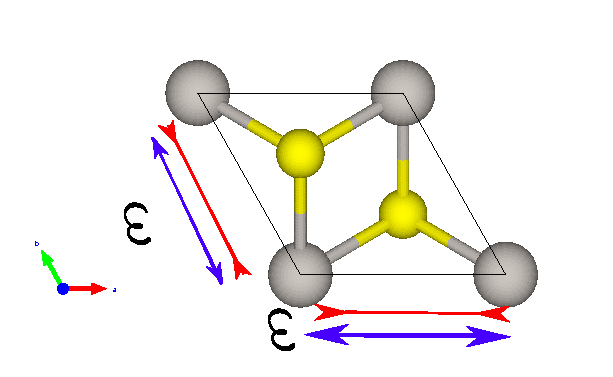
\epsfig{file=figMet/strainIso.eps, scale=0.9}
     	\label{Met:fig:strainiso}
     }
     \subfigure[]{
     	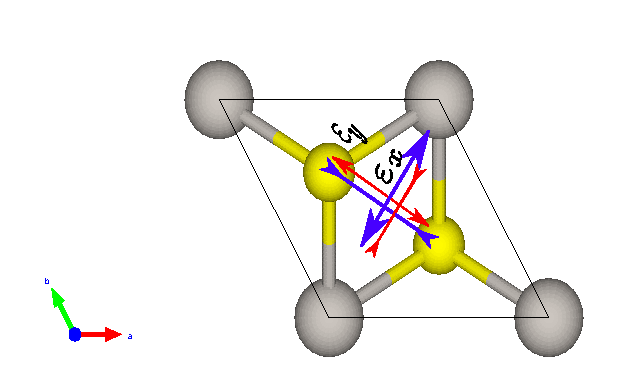
\epsfig{file=figMet/strainIAnis.eps, scale=0.9}
     	\label{Met:fig:strainanis}
     }	
     \caption[Deformaciones estudiadas.]{Deformaciones estudiadas en este trabajo. \ref{Met:fig:strainiso} Muestra la aplicaci\'on de una deformaci\'on isotr\'opica en direcci\'on de los ejes cristalinos y \ref{Met:fig:strainanis} una deformaci\'on dirigida en la direcci\'on de los ejes cartesianos.}
  \end{figure}
  \newline
  \par Como se dijo en las secci\'on \ref{subsec:nscf} es necesario utilizar la evaluaci\'on no auto-consistente para poder calcular la densidad de estados  y la estructura de bandas debido a que se requiere una cantidad mayor de puntos en el espacio rec\'iproco en comparaci\'on con el c\'alculo de la energ\'ia total del sistema. Para el caso de la densidad de estados  se utilizan $50 \times 50 \times 1 $ en la red de Monkhorst y Pack y  se utiliza un algoritmo de ajuste del tetraedro. Para el diagrama de bandas es necesario indicar el camino a seguir en la primera zona de Brillouin, en la figura \ref{Mat:fig:espacioK}. Se muestra \'esta indicando los puntos especiales y sus coordenadas en el espacio rec\'iproco. El camino que se sigui\'o para las estructuras de $PtS_2$ y $PtSe_2$ es $K-\Gamma-M-K$  y para las de $VS_2$ y $VSe_2$ es $\Gamma-M-K-\Gamma$. Es importante considerar que en el caso de que se aplique la deformaci\'on que se muestra en la figura \ref{Met:fig:strainanis}, el punto $M$ var\'ia linealmente de $(0.3518~0.3518~0)$ para $\varepsilon_x=-0.05$, a $(0.321~0.321~0)$ para $\varepsilon_x=0.04$. 
  \begin{figure}[hbt!]
  	\centering
  	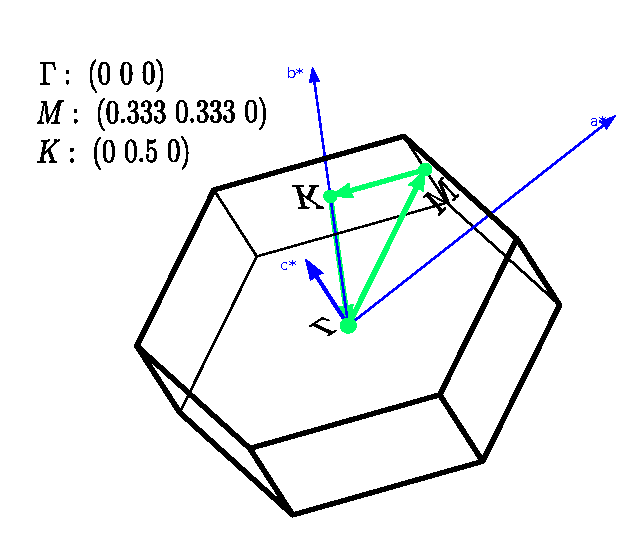
\epsfig{file=figMet/espacioK2.eps, width=8.0cm,height=8.0cm }
  	\caption[Puntos especiales en la zona de Brillouin.]{Mapeo en la primera zona de Brillouin indicando las coordenadas en el espacio rec\'iproco. Visualizado en XcrySDen}
    \label{Mat:fig:espacioK}
  \end{figure}
  \newline
  \par Para  generar las gr\'aficas de la estructura de bandas y de la densidad de estados, Quantum-Espresso cuenta con los  programas llamados bands.x y dos.x, los cuales toman los valores calculados por una evaluaci\'on no auto-consistente para poder generar las gr\'aficas correspondientes. Tambi\'en es importante obtener la densidad de estados proyectada en los orbitales at\'omicos (pDOS)  ya que de \'estos se puede observar cuales son los que contribuyen a la magnetizaci\'on. Para calcular el pDOS se utiliza el programa llamado projdos.x, el cual tambi\'en permite calcular la densidad de estados proyectada resuelta en el espacio rec\'iproco. De esta se puede obtener c\'omo es la contribuci\'on de cierto orbital a la estructura de bandas as\'i como cu\'ales bandas cuentan con spines orientados positiva y negativamente ($\uparrow,~\downarrow$).
  \newline
  \par Tambi\'en es de inter\'es visualizar la diferencia de densidad de electrones en el sistema para poder estudiar los enlaces qu\'imicos entre los \'atomos. Esta diferencia est\'a dada por la resta entre la densidad de electrones (ec. \ref{ec:densTot}) y la superposici\'on de las densidades at\'omicas.  As\'i mismo, tambi\'en es posible observar la densidad de la magnetizaci\'on resuelto en el espacio utilizando la ecuaci\'on \ref{ec:magn}, estas dos visualizaciones se pueden realizar utilizando una herramienta de Quantum Espresso llamada ``PostProc" (pp.x) y se puede observar en XcrySDen.
  
\section{M\'etodos experimentales} \label{Met:secmetExp}
\subsection{Montaje experimental}\label{Met:subsec:MontExp}
En la figura \ref{Met:fig:kerr} se muestra el montaje experimental utilizado para medir el efecto Kerr magneto-\'optico en configuraci\'on longitudinal. El sistema est\'a pensado para realizar mediciones variando el campo magn\'etico externo, las cuales son \'utiles para caracterizar las propiedades magn\'eticas del los materiales; es decir funcionar\'ia como un magnet\'ometro y se puede variar la longitud de onda lo cual es de gran utilidad para caracterizar los cambios en las propiedades electr\'onicas de los materiales bajo la influencia de un campo magn\'etico externo.
\begin{figure}[!hbt]
	\centering
	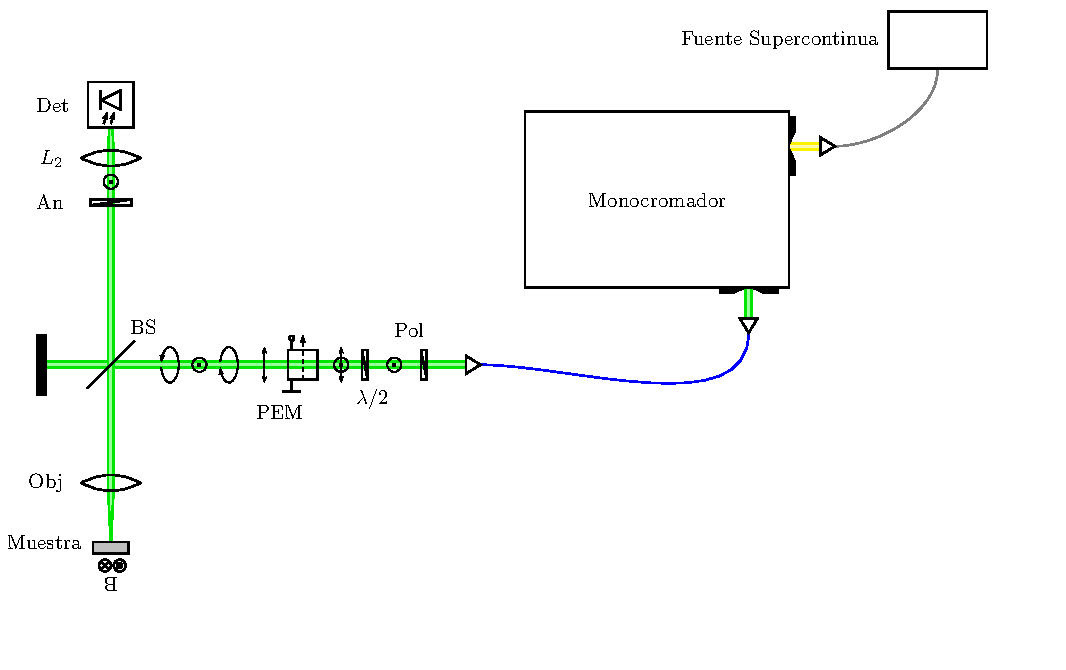
\includegraphics[scale=0.67]{figMet/diagrama/diagrama.pdf}
	\caption[Montaje experimental de espectroscop\'ia de efecto kerr magneto-\'optico.]{Montaje experimental para medir el efecto Kerr Mageto-\'optico en configuraci\'on longitudinal. La fiente supercontinua abarca un espectro de $430~nm $ a $2400~nm$ nm con una frecuencia de repetici\'on que var\'ia de $10~kHz $ a $80~MHz$ }
	\label{Met:fig:kerr}
\end{figure}
\newline
\par La fuente supercont\'inua es fabricada  por YSL Photonics y tiene como principales caracter\'isticas de que es posible controlar la frecuencia de repetici\'on y la potencia del pulso de salida, en el caso de este trabajo se utiliza una frecuencia de repetici\'on de $4 MHz$ al $30\%$  de la potencia total del pulso. El haz de esta fuente de luz sale colimado de una fibra \'optica y se introduce en un monocromador Acton 500M, el cual cuenta con tres rejillas de 300, 600 y 1200 $lineas/mm.$. En este caso se utilizan la de 1200 para el rango visible y la de 600 para el infrarrojo cercano. Este dispositivo se puede controlar por computadora mediante la comunicaci\'on serial. A la salida del monocromador se acopla el haz a una fibra \'optica para introducirlo en el sistema de medici\'on. A la salida de la fibra se utiliza una lente para colimar el haz y  posteriormente se coloca un polarizador Wollatson que est\'a orientado a $0\degree$ con respecto a la horizontal de tal forma que la polarizaci\'on del haz de salida est\'a polarizada linealmente. Debido a que es necesario orientar la direcci\'on de polarizaci\'on a $45 \degree$ se utiliza un retardador de media onda colocado en una montura rotatoria K10CR1/M de Thorlabs la cual puede ser controlada remotamente por medio del software Kinesis. Posteriormente se utiliza un modulador fotoel\'astico (PEM), cuyo eje r\'apido est\'a a $90 \degree$ con respecto al eje horizontal y cuyo  modelo es PEM-90 de Hinds Instruments, al cual se le puede controlar el retardo que se le induce al haz. En este caso se le agrega un retardo de $\lambda/4$ con una frecuencia de operaci\'on es de $42~ MHz$. Tambi\'en es posible controlarlo remotamente por medio de un puerto serial. Una vez que el haz sale del PEM se estar\'a modulando la polarizaci\'on del haz cambiando de una lineal a circular. Posteriormente se utiliza un beamsplitter para dirigir el haz hacia la muestra y se utiliza un objetivo de microscopio de 50x para enfocar la luz en la muestra que est\'a colocada entre un par de bobinas para inducir campo magn\'etico en la muestra en las direcciones marcadas en el figura \ref{Met:fig:kerr} y cuya magnitud se encuentra entre 0 y 0.7 mT. Dicho campo magn\'etico es controlado  variando la intensidad de corriente que circula a travez las bobinas y se cuenta con un controlador manual que tiene control PID para dicha corriente. El haz reflejado pasa por un segundo polarizador orientado a $90 \degree$ que funciona como analizador ya que convierte los cambios en polarizaci\'on en un cambio de intensidad y por \'ultimo, se utiliza una lente para enfocar la luz en un detector avalancha de Silicio de modelo  Thorlabs. La salida del detector se conecta a un mult\'imetro Keithley 720  y a un amplificador Lock in (sr510 Stanford Reseach) que se encuentra sincronizado con la frecuencia de operaci\'on del PEM. Ambos dispositivos pueden se pueden comunicar a una computadora por medio de un puerto GPIB-serial.
\newline 
\par Se utiliz\'o el an\'alisis de matrices de Jones (Ap\'endice \ref{Jones:App}) para deducir una expresi\'on de la intensidad de la luz que llega al detector y  se obtiene un par de expresiones para las razones de la intensidad que detecta el lock in cuando se encuentra sincronizado con el primer y segundo arm\'onico del retardo del modulador fotoel\'astico (ecs. \ref{Jones:ec:divI1} y\ref{Jones:ec:divI2} ):
\begin{eqnarray}
I_1/I_0 &=& 4 J_1 (\Psi_0) ~tan(\varPsi) ~(\theta_k ~sin(\Delta) - \eta_k~ cos(\Delta)) \label{Met:ec:divI1}\\
I_2/I_0 &=& -4 J_2 (\Psi_0) ~tan(\varPsi) ~(\theta_k~cos(\Delta) + \eta_k ~ sin(\Delta)) \label{Met:ec:divI2}.
\end{eqnarray}
En este caso $I_0$ es detectada por el mult\'imetro digital. Se utiliza un programa desarrollado en LabVIEW (Ap\'endice \ref{AppKerrAuto}), el cual es utilizado para controlar el monocromador  y el PEM as\'i como para adquirir informaci\'on del amplificador lock in y del mult\'imetro. Una vez que se tienen estos valores se realiza la raz\'on entre el valor del lock in y el del mult\'imetro de tal forma que se obtienen las expresiones \ref{Met:ec:divI1} y \ref{Met:ec:divI2} dependiendo de que si el lock in est\'a sincronizado a $f$ o $2f$.  Este programa le permite al usuario realizar mediciones variando la longitud de onda o medir el ciclo de hist\'eresis variando el campo magn\'etico externo aplicado a la muestra.
\subsection{An\'alisis de los datos experimentales} \label{Met:subsec:AnExp}
 De acuerdo con las ecuaciones \ref{Met:ec:divI1} y \ref{Met:ec:divI2} se observa que es necesario realizar un an\'alisis mas detallado debido a que no es posible obtener los valores  para la rotaci\'on ($\theta_k$) y la elipticidad ($\varepsilon_k$) Kerr de forma directa, dado  que en estas expresiones aparecen mezcladas en ambas ecuaciones. Es posible encontrar los valores para la rotaci\'on  y la elipticidad si se tratan las expresiones \ref{Met:ec:divI1} y \ref{Met:ec:divI2} como un sistema de ecuaciones, para lo cual es necesario conocer los valores de $\varPsi (eV)$ y $\Delta (eV)$ del beamsplitter. Estos valores fueron posible conocerlos realizando una medici\'on de elipsometr\'ia a $70\degree$ cuyos valores se observan en la figura \ref{Met:fig:ElipBS} junto con su ajuste realizado con el programa WVASE. En base con este ajuste es posible estimar los valores de $\varPsi (eV)$ y $\Delta (eV)$ para $45 \degree$ con ayuda de WVASE que se muestran en la figura \ref{Met:fig:ElipBS45}. Como se puede observar estos dos par\'ametros presentan grandes variaciones en todo el espectro  por lo que fue necesario implementar una rutina en Python (Ap\'endice \ref{App:Py}) para poder obtener  los valores de la elipticidad  y el \'angulo Kerr resolviendo el sistema de ecuaciones (\ref{Met:ec:divI1} y \ref{Met:ec:divI2}).
\begin{figure}[!hbt]
	\centering
	\subfigure[valores de $\Psi$]{
	\includegraphics[scale=0.75]{figMet/figElips/grafPsi}
	\label{Met:fig:PsiBS}
	}
    \subfigure[valores de $\Delta$]{
    	\includegraphics[scale=0.75]{figMet/figElips/grafTheta}
    	\label{Met:fig:DeltaBS}
    }
\caption[Gr\'aficas de $\Psi$ y $\Delta$ del beamspliter a $70 \degree$.]{valores experimentales a $70\degree$  para $\Psi$ y $\Delta$ del beamsplitter en funci\'on de la energ\'ia del fot\'on con su ajuste.} 
\label{Met:fig:ElipBS}
\end{figure}
\begin{figure}[!hbt]
	\centering
	\includegraphics[scale=1.3]{figMet/figElips/grafPsidelta45.pdf}
	\caption[Gr\'aficas de $\Psi$ y $\Delta$ del beamspliter a $70 \degree$.]{valores calculados a $45\degree$  para $\Psi$ y $\Delta$ del beamsplitter.}
	\label{Met:fig:ElipBS45}
\end{figure}
\newline
\subsection{Muestras}\label{Met:subsec:Muest}
La muestra utilizada en para comprobar que el funcionamiento del sistema de espectroscop\'ia de efecto Kerr Magneto-\'optico es una aleaci\'on de Hierro, Cobalto y Boro (CoFeB)	en donde las concentraciones son del $20~\%$ para el Cobalto y el Boro y del $60~\%$ para el Hierro. Dado que se aplica un campo magn\'etico externo B es necesario conocer la respuesta en funci\'on del campo magn\'etico $H$, es conocido que se relacionan con la siguiente expresi\'on \cite{magMan_1}
\begin{equation}
	\pmb{B}_{[T]}=\mu_0 (\pmb{H}_{[A ~m^{-1}]}+\pmb{M}_{[A ~m^{-1}]} + \pmb{H}_d ),
	\label{Met:ec:BSI}
\end{equation}  
	en donde $\pmb{B}$ es el campo magn\'etico externo, $\pmb{H}$ es el campo  magn\'etico inducido, $\pmb{M}$ es la magnetizaci\'on y $\pmb{H}_d$ es el campo desmagnetizante definido como $\pmb{H}_d = -N_d \pmb{M}$ en donde   $N_d$ es el factor desmagnetizante que generalmente depende de la geometr\'ia de la estructura, la ecuaci\'on \ref{Met:ec:BSI} puede ser escrita en unidades CGS \cite{magMan_1}
    \begin{equation}
    	\pmb{B}_{[Gauss]}= \pmb{H}_{[Oe]}+4 \pi \pmb{M}_{[emu ~cm^{-3}]} +\pmb{H}_d ,
    	\label{Met:ec:BCGS}
    \end{equation}	
en donde hay que considerar que las unidades SI se relacionan con las CGS de la siguiente manera \cite{magMan_2}:
\begin{eqnarray}
	1~T&=& 10^{-4}~ Gauss \nonumber \\
	1~ A~m^{-1} &=& 4 \pi \times 10^{-3}~ Oe \nonumber \\
	1~emu~cm^{-3} &=& 10^{-3} A~ m^{-1}. \nonumber
\end{eqnarray}
Dado que se trata de una pel\'icula delgada de CoFeB en este caso el factor desmagnetizante en el caso que el campo  magnético  externo $\pmb{B}$ se dirija en la direcci\'on $x$ se obtiene \cite{magMan_1}, $N_{d,y}=N_{d,x}=0$ y $N_{d,z}=4\pi$ en unidades CGS, entonces la ecuaci\'on \ref{Met:ec:BCGS} se puede aproximar a
\begin{equation*}
	\pmb{B} \approx \pmb{H}.
\end{equation*} 
  \endinput

		\chapter{Resultados de simulaciones} \label{cap:Sim}
En el presente cap\'itulo se exponen los resultados de las simulaciones realizadas en esta tesis. En la secci\'on \ref{Sim:sec:MSdef} se muestran las propiedades magn\'eticas de los materiales sin defectos. En la secci\'on \ref{Sim:sec:MdefVac} se estudia el efecto de introducir una vacancia del metal de transición en el sistema. En la secci\'on \ref{Sim:sec:Str} se estudia el efecto de inducir una deformaci\'on en los sistemas de acuerdo con lo descrito en la subsecci\'on \ref{Met:subsec:detcomp}.
\section{An\'alisis de materiales sin defectos} \label{Sim:sec:MSdef}
\subsection{PtSe\textsubscript{2}} \label{Sim:subsec:ptse2celu}
En la figura \ref{Sim:fig:estptse2} se muestra la estructura proyectada en la direcci\'on $c$ y de lado (direcciones $b$ y $c$). se observa que tiene una estructura $1T$ y  comparando los par\'ametros estructurales obtenidos con otros ya observados anteriormente (tabla \ref{Sim:tabla:ptse2est}).
\begin{table}
	\centering
	\caption[Comparaci\'on de par\'ametros estructurales del PtSe\textsubscript{2}.]{comparaci\'on de la constante de red $a_0$, y de enlaces $d_{Pt-Se}$, $d_{Se-Se}$, el \'angulo entre los \'atomos de Platino y Selenio y el tama\~no de la brecha prohibida, estos datos son   comparados con resultados de otras simulaciones y de resultados experimentales. }
	\begin{tabular}{|c|c|c|c|c|c|}
	\hline
		    & $a_0~(\AA)$   & $d_{Pt-Se}~(\AA)$  & $d_{Se-Se}~(\AA)$  &  $\theta_{Se-Pt-Se}~(grado)$ & $E_g~(eV)$ \\
    \hline
    \hline
    calc.   & $3.7610$& $2.5343 $     & $3.3978 $  & $95.81$              & $1.3911 ~(1.1841)$\\
    ref. \cite{doi:10.1063/1.4955468}    & $3.75$& $2.53 $     & $3.40 $  & $95.67$              & $1.4 ~(1.2)$\\
    exp. \cite{datexpPt}   & $3.73$& $2.51 $     & $3.35 $  & $96.13$              & $1.2$\\
    \hline

	\end{tabular}
    \label{Sim:tabla:ptse2est}
\end{table}
\newline
\begin{figure}[!hbt]
	\centering
	\subfigure[vista de arriba]{
		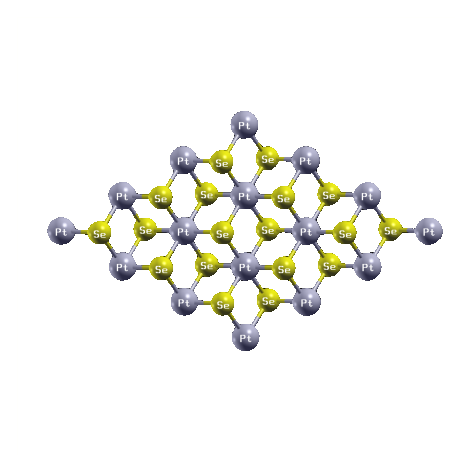
\epsfig{file=figRes/PtSe2/est/est1.eps, width=6cm, height=6cm}
		\label{Sim:fig:estptse2arr}
	}
    \subfigure[vista de lado]{
    	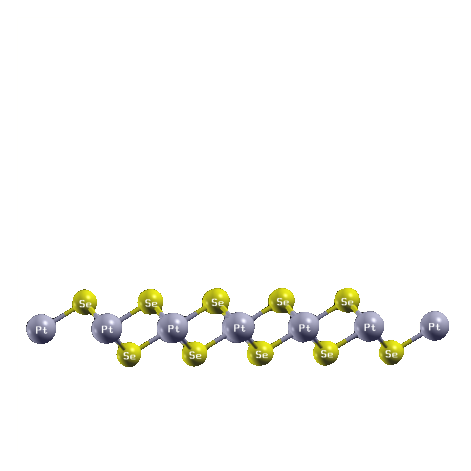
\epsfig{file=figRes/PtSe2/est/est2.eps, width=6cm, height=6cm}
    	\label{Sim:fig:estptse2lado}
    }
   \caption[Vista de la supercelda de PtSe\textsubscript{2}.]{Vista de la estructura de $PtSe_2$ en la que se repiten 3 veces la celda unitaria en dos direcciones.}
   \label{Sim:fig:estptse2}
\end{figure}
\newline
En la figura \ref{Sim:fig:bandasptse2} se muestra el diagrama de bandas con acople spin-\'orbita (fig \ref{Sim:fig:bandSocptse2}) y sin este  efecto (fig. \ref{Sim:fig:bandnoSocptse2}). La principal caracter\'istica de este material es que en el caso de una mono-capa es un semiconductor indirecto, encontr\'andose el m\'inimo de la banda de conducci\'on entre los puntos $\Gamma$ y $M$ y el m\'aximo de la banda de valencia se encuentra entre el punto $M$ y $\Gamma$ (~$0.20 \AA^{-1}$ del punto $\Gamma$); desplazándose  al punto $\Gamma$ cuando se incluye el efecto de spin-\'orbita, debido a que  las bandas que son degeneradas en el punto $\Gamma$  en la banda de valencia,  se separan $\Delta_{so}^{v,\Gamma}=333.41 ~meV$ y en el punto $K$ se distancian $\Delta_{so}^{v,K}=163 ~meV$. Adem\'as  se observa que la separaci\'on entre las dos primeras bandas de conducci\'on de $\Delta_{so}^{c,\Gamma} = 57.48~ meV$ en el punto $\Gamma$ y de $\Delta_{so}^{c,K} = 2.1 ~meV$ en el punto $K$, los cuales son mas peque\~nos que en la banda de valencia. Estos rompimientos de la degeneraci\'on provocan que el tama\~no de la brecha prohibida se reduzca a $1.2 ~eV$. Si se observa la densidad de estados, se puede notar que la banda de valencia est\'a formada principalmente por los electrones de  orbitales $d$ del Platino, con excepci\'on  del m\'aximo de la banda de valencia el cual est\'a formado mayoritariamente por los orbitales $p$ del Selenio, con una mezcla de orbitales $d$ del Platino. En el caso de la banda de conducci\'on, la contribuci\'on de ambos orbitales es casi la misma y su distribuci\'on en el diagrama de bandas se observa en la figura \ref{Sim:fig:pdosPtse2cU}, la cual est\'a formada por el mapeo de la densidad de estados proyectada sobre el respectivo orbital en la primera zona de Brillouin.

\begin{figure}[!hbt]
	\centering
	\subfigure[con acople spin-\'orbita]{
		\includegraphics[scale=1]{figRes/PtSe2/bandas/bandasDOS.pdf}
		\label{Sim:fig:bandSocptse2}
	}
    \subfigure[sin acople spin-\'orbita]{
    	\includegraphics[scale=1]{figRes/PtSe2/bandas/noSOC/bandasDOSnoSoc.pdf}
    	\label{Sim:fig:bandnoSocptse2}
    }
\caption[Diagrama de bandas y densidad de estados de la celda unitaria del PtSe\textsubscript{2}.]{Gr\'aficas del diagrama de bandas y la densidad de estados del PtSe\textsubscript{2} (\ref{Sim:fig:bandSocptse2}) incluyendo el acople spin-\'orbita y (\ref{Sim:fig:bandnoSocptse2}) sin este efecto.}
\label{Sim:fig:bandasptse2}
\end{figure}



 Dado que la magnetizaci\'on es cero, se puede decir que el material es no-magn\'etico incluso si se incluye el efecto de spin-\'orbita. Esto se puede explicar debido a que el Platino, que  tiene seis electrones del orbital $d$  $(Pt^{4+})$ se encuentran de forma estable en el estado $t_{2g}$ \cite{doi:10.1063/1.4955468} y por lo tanto, no cuentan con   un orden magn\'etico entre los \'atomos de Platino. 
\begin{figure}[!hbt]
	\centering
	\includegraphics[scale=1]{figRes/PtSe2/bandas/projbandorb/orbproj.pdf}
	\caption[Distribuci\'on de orbitales $d$ y $p$ del Platino y Selenio respectivamente el ep PtSe\textsubscript{2}.]{Distribuci\'on de los orbitales $d$ del platino y $p$ del Selenio en el PtSe\textsubscript{2} sin el efecto de spin-\'orbita y considerando una densidad de estados mayor a 0.1 estados/eV. }
	\label{Sim:fig:pdosPtse2cU}
\end{figure}
\subsection{PtS\textsubscript{2}} \label{Sim:subsec:pts2celu}
Un material muy similar  es el Disulfuro de Platino el cual cuenta con la misma estructura que el di seleniuro de platino. En la tabla \ref{Sim:tabla:pts2est} se muestra la comparaci\'on con los datos experimentales y de otras simulaciones con los obtenidos en este trabajo y se puede observar que estos resultados son muy similares a los reportados de simulaciones y de par\'ametros experimentales. En el caso de la brecha prohibida se obtiene tambi\'en un valor parecido al obtenido experimentalmente. Se puede notar que en comparaci\'on con los datos correspondientes al PtSe\textsubscript{2}, el PtS\textsubscript{2} tiene una constante de red mas peque\~na as\'i como los dem\'as par\'ametros estructurales. En cambio el tama\~no de la brecha prohibida es mayor en el PtS\textsubscript{2}, lo cual podr\'ia indicar que las interacciones entre los \'atomos de Azufre y Platino es mayor que el caso del Platino y Selenio.
\begin{table}
	\centering
	\caption[Comparaci\'on de par\'ametros estructurales del PtS\textsubscript{2}.]{Se comparan los mismos par\'ametros que en el cuadro \ref{Sim:tabla:ptse2est} pero se cambia el \'atomo de Selenio por uno de azufre }
	\begin{tabular}{|c|c|c|c|c|c|}
		\hline
		& $a_0~(\AA)$   & $d_{Pt-S}~(\AA)$  & $d_{S-S}~(\AA)$  &  $\theta_{S-Pt-S}~(grado)$ & $E_g~(eV)$ \\
		\hline
		\hline
		calc.   & $3.5785$& $2.4072 $     & $3.2207 $  & $96.04$              & $1.3911 ~(1.724)$\\
		ref. \cite{doi:10.1021/jp405808a,DU201}    & $3.57$& $2.40 $     & $3.21 $  & $96.18$              & $1.81 ~(1.76)$\\
		exp. \cite{datexpPt,https://doi.org/10.1002/adma.201504572}   & $3.5432$& $2.34 $     & $3.07 $  & $98.21$              & $1.6$\\
		\hline
		
	\end{tabular}
	\label{Sim:tabla:pts2est}
\end{table}
%\newline
\newline
\par En la figura \ref{Sim:fig:bandaspts2} se muestra la estructura de bandas del PtS\textsubscript{2} con efectos de acople spin-\'orbita (fig. \ref{Sim:fig:bandSocpts2}) y sin este (fig. \ref{Sim:fig:bandnoSocpts2}). Se puede notar que este material es un semiconductor indirecto con el m\'inimo de la banda de conducci\'on que se encuentra entre el punto $\Gamma$ y $M$ al igual que con el PtS\textsubscript{2}. Pero en el caso de la banda de valencia no sucede lo mismo ya que cuando se incluyen los efectos de spin \'orbita, el m\'aximo de la banda de valencia no se encuentra en el punto $\Gamma$ sino que se localiza entre el punto $\Gamma$ y $K$ a $0.23 \AA^{-1}$ del punto $\Gamma$. En cuanto al rompimiento de la degeneraci\'on por el efecto de spin-\'orbita, se observa una separaci\'on entre las bandas del m\'aximo de la banda de valencia en el punto $\Gamma$ que es $\Delta_{so}^{v,\Gamma}= 207.1~ meV$ y en el punto $K$ es de $\Delta_{so}^{v,K}= 195~ meV$. Para el caso de  la separaci\'on entre las dos  primeras bandas de conducci\'on  en el punto $\Gamma$ es de $\Delta_{so}^{c,\Gamma}= 256~ meV$ y en el punto $K$ es de  $\Delta_{so}^{v,K}= 107~ meV$. Comparando estos valores con los obtenidos para el PtSe\textsubscript{2} se observa que, a excepci\'on del punto $\Gamma$ en la banda de valencia,  son mayores las separaciones $\Delta_{so}$ en el PtS\textsubscript{2}, debido  a que a diferencia del PtSe\textsubscript{2} no sucede una disminuci\'on tan marcada de los estados correspondientes a los orbitales $d$ del Platino cerca del m\'aximo de la banda de valencia.  En la banda de conducci\'on es ligeramente  mayor la poblaci\'on de estos electrones $d$ que la de los electrones del orbital $p$ del Selenio. En la figura \ref{Sim:fig:pdosPts2cU} se muestra la distribuci\'on de los estados de dichos dos orbitales en el diagrama de bandas, en el que se puede notar que los electrones $d$ del platino se encuentran mas distribuidos en el m\'aximo de la banda de valencia en comparaci\'on del PtSe\textsubscript{2}. El efecto de spin-\'orbita provoca que el tama\~no de la brecha prohibida se reduzca a $1.72~ eV$ el cual es un valor cercano al medido experimentalmente\cite{https://doi.org/10.1002/adma.201504572}.
\newline
En el caso del c\'alculo de la magnetizaci\'on, se encontr\'o que es $0 ~\mu_{B}/celda$, el cual es el mismo resultado que se obtuvo para el PtSe\textsubscript{2} y el motivo de que \'este material no sea magn\'etico es el mismo que para el PtSe\textsubscript{2}.
\begin{figure}[!hbt]
	\centering
	\subfigure[con acople spin-\'orbita]{
		\includegraphics[scale=1]{figRes/PtS2/bandas/celu/soc/bandasDOS.pdf}
		\label{Sim:fig:bandSocpts2}
	}
	\subfigure[sin acople spin-\'orbita]{
		\includegraphics[scale=1]{figRes/PtS2/bandas/celu/nosoc/bandasDOSnoSoc.pdf}
		\label{Sim:fig:bandnoSocpts2}
	}
	\caption[Diagrama de bandas y densidad de estados de la celda unitaria del PtS\textsubscript{2}.]{Gr\'aficas del diagrama de bandas y la densidad de estados del PtS\textsubscript{2} (\ref{Sim:fig:bandSocpts2}) incluyendo el acople spin-\'orbita y (\ref{Sim:fig:bandnoSocpts2}) sin este efecto.}
	\label{Sim:fig:bandaspts2}
\end{figure}
\begin{figure}[!hbt]
	\centering
	\includegraphics[scale=1]{figRes/PtS2/bandas/celu/projbandas/orbproj.pdf}
	\caption[Distribuci\'on de orbitales $d$ y $p$ del Platino y Selenio respectivamente el ep PtS\textsubscript{2}.]{Distribuci\'on de los orbitales $d$ del platino y $p$ del Selenio en el PtS\textsubscript{2} sin el efecto de spin-\'orbita y considerando una densidad de estados mayor a 0.1 estados/eV. }
	\label{Sim:fig:pdosPts2cU}
\end{figure}

\begin{table}
	\centering
	\caption[Comparaci\'on de par\'ametros estructurales del VSe\textsubscript{2}.]{Se comparan los mismos par\'ametros que en el cuadro \ref{Sim:tabla:ptse2est} pero se cambia el \'atomo de Platino por uno de Vanadio  y sin considerar el tama\~no de la brecha prohibida}
	\begin{tabular}{|c|c|c|c|c|}
		\hline
		& $a_0~(\AA)$   & $d_{V-Se}~(\AA)$  & $d_{Se-Se}~(\AA)$  &  $\theta_{Se-V-Se}~(grado)$ \\
		\hline
		\hline
		calc.   & $3.3403$& $2.4924 $     & $3.7 $  & $84.15$ \\
		ref. \cite{doi:10.1021/jp405808a}    & $3.32$& $2.48 $     & $3.7 $  & $83.81$ \\
		exp. \cite{expVse}   & $3.355$& $2.47 $     & $3.627 $  & $85.53$\\
		\hline
		
	\end{tabular}
	\label{Sim:tabla:VSe2est}
\end{table}
\subsection{VSe\textsubscript{2}} \label{Sim:subsec:vse2cU}
Los resultados estructurales y su comparaci\'on con otros trabajos se muestran en la tabla \ref{Sim:tabla:VSe2est}, se puede observar que los valores obtenidos son menores a los dos materiales analizados anteriormente, aunque se sigue manteniendo la estructura 1T estable. En este no existe una brecha prohibida  lo que indica que este material  se comporta como un metal. En la figura \ref{Sim:fig:bandasVSe2} se observan el diagrama de bandas con el efecto de spin-\'orbita(fig. \ref{Sim:fig:bandSocVSe2}) y sin este (fig \ref{Sim:fig:bandnoSocVse2}). En dicha situación  se muestran las bandas orientadas con el spin ($1/2,~ \uparrow$) y con el spin ($-1/2,~ \downarrow$) y es posible observar que el n\'umero de estados no es el mismo para estas dos componentes,  provocando una magnetizaci\'on de $0.62~ \mu_B / celda$.
\begin{figure}[!hbt]
	\centering
	\subfigure[con acople spin-\'orbita]{
		\includegraphics[scale=1]{figRes/VSe2/bandas/celU/soc/bandasDOS.pdf}
		\label{Sim:fig:bandSocVSe2}
	}
	\subfigure[sin acople spin-\'orbita]{
		\includegraphics[scale=0.9]{figRes/VSe2/bandas/celU/nosoc/bandasDOSnoSoc.pdf}
		\label{Sim:fig:bandnoSocVse2}
	}
	\caption[Diagrama de bandas y densidad de estados de la celda unitaria del VSe\textsubscript{2}.]{Gr\'aficas del diagrama de bandas y la densidad de estados del VSe\textsubscript{2} (\ref{Sim:fig:bandSocVSe2}) incluyendo el acople spin-\'orbita y (\ref{Sim:fig:bandnoSocVse2}) sin este efecto.}
	\label{Sim:fig:bandasVSe2}
\end{figure}
\newline
Si se observa la figura \ref{Sim:fig:bandSocVSe2} se nota que las separaciones que induce el efecto de spin- \'orbita el las bandas por debajo del nivel de Fermi  son muy peque\~nas en los puntos $\Gamma$, $M$ y $K$, aunque estas aumentan el las posiciones intermedias entre estos, lo cual   permite separar las bandas degeneradas que corresponden a distintos spines (fig \ref{Sim:fig:bandnoSocVse2}). adem\'as, se puede observar en la densidad de estados que estas bandas est\'an compuestas por los electrones en el orbital $p$ de Selenio mezclados con electrones del orbital $d$ del vanadio a diferencia de   los estados cercanos y superiores al nivel de Fermi  que est\'an compuestos por los electrones del orbital $d$ del Vanadio, principalmente. Tal y como se muestra en la densidad de estados (fig. \ref{Sim:fig:bandnoSocVse2}) los orbitales $d$ de Vanadio contribuyen  considerablemente a la aparici\'on del momento magn\'etico distinto de cero. En la figura \ref{Sim:fig:pDOSvVse2} se aprecia que la mayor contribuci\'on a los estados ocupados cercanos al nivel de Fermi, proviene del orbital $d_{z^2}$ y en los estados mas lejanos por los orbitales $d_{zx}$ y $d_{zy}$; por lo que se espera que los electrones de los estados ocupados tengan el spin orientado en la direcci\'on perpendicular al plano de la muestra. Los estados no ocupados esencialmente est\'an formados por los orbitales $d_{x^2 -y^2}$ y $d_{xy}$, en donde los \'atomos de vanadio aportan una magnetizaci\'on de $0.61~ \mu_{B}$.   
\begin{figure}[!hbt]
	\centering
	\includegraphics[scale=1]{figRes/VSe2/bandas/celU/nosoc/pdosV.pdf}
	\caption[Densidad de estados proyectada de los orbitales $d$ del vanadio en VSe\textsubscript{2}.]{densidad de estados parcial de los orbitales $d$ del \'atomo de Vanadio en VSe\textsubscript{2}, la flecha azul y roja indican la densidad de estados de los spines $1/2$ y $-1/2$ respectivamente.}
	\label{Sim:fig:pDOSvVse2}
\end{figure}
\newline
En la figura \ref{Sim:fig:pDOSseVse2} se observa la densidad de estados proyectada en los orbitales $p$ del \'atomo de Selenio, se puede observar que los orbitales $p_{x}$ son los que contribuyen a los estados en el VSe\textsubscript{2}, as\'i mimo se nota que los \'atomos de selenio aportan una magnetizaci\'on de $ -0.038~ \mu_{B}$.
\begin{figure}[!hbt]
	\centering
	\includegraphics[scale=1]{figRes/VSe2/bandas/celU/nosoc/pdosSe.pdf}
	\caption[Densidad de estados proyectada de los orbitales $p$ del Selenio en VSe\textsubscript{2}.]{densidad de estados parcial de los orbitales $p$ del \'atomo de Selenio en VSe\textsubscript{2}, la flecha azul y roja indican la densidad de estados de los spines $1/2$ y $-1/2$ respectivamente.}
	\label{Sim:fig:pDOSseVse2}
\end{figure}
%\newline
\par En la figura \ref{Sim:fig:distmagnVse2} se muestra la distribuci\'on de spines  y se puede notar que en los \'atomos de Vanadio se concentran los  valores positivos para el spin y en los \'atomos de Selenio se concentra una peque\~na contribuci\'on negativa que, de acuerdo a la densidad de estados, esta proviene de el orbital $p_x$; as\'i mismo, se observa una peque\~na contribuci\'on positiva que se puede atribuir a los orbitales $p_z$.
\begin{figure}[!hbt]
	\centering
	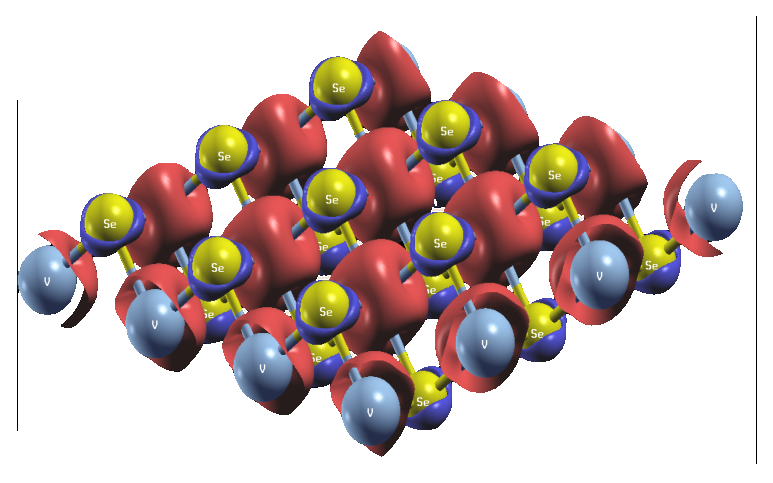
\epsfig{file=figRes/VSe2/vse2magz.eps, scale=0.65}
	\caption[Distribuci\'on de spin en VSe\textsubscript{2}]{Distribuci\'on  de spin en el VSe\textsubscript{2} visualizada con XcrySDen, en donde se muestra un valor de iso superficie de $\pm 0.002$, en donde el color rojo indica un valor positivo y el azul el negativo.}
	\label{Sim:fig:distmagnVse2}
\end{figure}
\subsection{VS\textsubscript{2}} \label{Sim:subsec:VS2}
Este material en la estructura 1T tiene características muy similares al VSe\textsubscript{2}, en la tabla \ref{Sim:tabla:VS2est} se muestran los par\'ametros estructurales calculados en este trabajo y su comparaci\'on con otras simulaciones. Para este material no existen muchos estudios experimentales y es por esta raz\'on  que solamente se muestra el tama\~no de red, el cual es muy cercano al calculado. De igual forma los par\'ametros calculados en este trabajo son muy parecidos a  otras simulaciones realizadas anteriormente.
%\newline

\begin{table}
	\centering
	\caption[Comparaci\'on de par\'ametros estructurales del VS\textsubscript{2}.]{Par\'ametros estructurales para el VS\textsubscript{2} y su comparaci\'on con otras simulaciones y con datos obtenidos por experimentos.}
\begin{tabular}{|c|c|c|c|c|}
	\hline
	& $a_0~(\AA)$   & $d_{V-S}~(\AA)$  & $d_{S-S}~(\AA)$  &  $\theta_{S-V-S}~(grado)$ \\
	\hline
	\hline
	calc.   & $3.1939$& $2.3556 $     & $3.4632 $  & $85.367$ \\
	ref. \cite{doi:10.1021/jp405808a}    & $3.17$& $2.35 $     & $3.46 $  & $85.04$ \\
	exp. \cite{C9QI01142K}   & $3.22$& $-- $     & $-- $  & $--$\\
	\hline
	
\end{tabular}
\label{Sim:tabla:VS2est}
\end{table}

\par En la figura \ref{Sim:fig:bandasVS2} se muestra el diagrama de bandas  con el efecto de spin-\'orbita(fig. \ref{Sim:fig:bandSocVS2}) y sin este fig. (\ref{Sim:fig:bandnoSocVs2}). En el caso en el que considera el acople spin-\'orbita se observa el mismo fen\'omeno que en el caso del VSe\textsubscript{2}, es decir en los puntos de alta simetr\'ia ($\Gamma$, $K$ y $M$) el rompimiento de la degeneraci\'on en las bandas con distinto spin (se pueden observar en la Fig. \ref{Sim:fig:bandnoSocVs2}) es muy peque\~no y en las posiciones intermedias entre estos puntos aumenta la separaci\'on entre estas bandas,  permitiendo diferenciar entre bandas de distinto spin. En el caso de los estados por encima del nivel de Fermi, se tienen un conjunto bien determinado por bandas orientadas con spin $\uparrow$ y otras con spin $\downarrow$ y est\'an formadas principalmente por el orbital $d$ del Vanadio. En general se observa que la separaci\'on entre las bandas son peque\~nas debido a que el \'atomo de Vanadio no es muy pesado en comparaci\'on con el Platino.
\newline %\newline
\par En el caso del c\'alculo de la magnetizaci\'on se encontr\'o que este material es ferromagn\'etico debido a que la magnetizaci\'on tiene un valor de $0.55 ~\mu_{B}/celda$, el cual es un valor menor a que se obtuvo en el caso de VSe\textsubscript{2}. Observando la densidad de estados en la figura \ref{Sim:fig:bandnoSocVs2} se nota que en los estados por debajo del nivel de Fermi, el orbital $d$ del \'atomo de vanadio esta un poco delocalizado y  la poblaci\'on de los orbitales $p$ del \'atomo de Azufre es muy similar al del vanadio, lo cual podr\'ia sugerir que estos orbitales se hibridizan  y forman enlaces covalentes entre estos dos \'atomos y este es un fen\'omeno que tambi\'en se observa en el los materiales descritos anteriormente.
\begin{figure}[!hbt]
	\centering
	\subfigure[con acople spin-\'orbita]{
		\includegraphics[scale=1]{figRes/VSe2/bandas/celU/soc/bandasDOS.pdf}
		\label{Sim:fig:bandSocVS2}
	}
	\subfigure[sin acople spin-\'orbita]{
		\includegraphics[scale=0.9]{figRes/VS2/celdaU/estructura electronica/noSOC/bandasDOSnoSoc.pdf}
		\label{Sim:fig:bandnoSocVs2}
	}
	\caption[Diagrama de bandas y densidad de estados de la celda unitaria del VS\textsubscript{2}.]{Gr\'aficas del diagrama de bandas y la densidad de estados del VS\textsubscript{2} (\ref{Sim:fig:bandSocVS2}) incluyendo el acople spin-\'orbita y (\ref{Sim:fig:bandnoSocVs2}) sin este efecto.}
	\label{Sim:fig:bandasVS2}
\end{figure}
\newline

\par Estudiando los orbitales $d$ del \'atomo de vanadio (fig. \ref{Sim:fig:pDOSvVs2}) se observa que, al igual que en el caso del VSe\textsubscript{2},  el orbital $d_{z^2}$ es el que tiene la mayor contribución a los  estados por debajo del nivel de Fermi y que por lo general se encuentran delocalizados. Para los estados  desocupados estos est\'an formados por orbitales $d_{x^2-y^2}$ y $d_{xy}$, los cuales est\'an muy localizados. Dichos orbitales tambi\'en tienen importantes contribuciones en los estados que se encuentran ocupados, los orbitales $d_{zx}$ y $d_{zy}$ tienen contribuciones importantes en los estados m\'as cercanos al n\'ucleo y si se toma en consideraci\'on que los estados orientados en la direcci\'on $z$, se espera que los spines est\'en orientados en esa direcci\'on. La magnetizaci\'on que aporta el \'atomo de Vanadio es de $ 0.5 ~\mu_{B} $.
\begin{figure}[!hbt]
	\centering
	\includegraphics[scale=1]{figRes/VSe2/bandas/celU/nosoc/pdosV.pdf}
	\caption[Densidad de estados proyectada de los orbitales $d$ del Vanadio en el VS\textsubscript{2}.]{Densidad de estados parcial de los orbitales $d$ del \'atomo de Vanadio en VSe\textsubscript{2}, la flecha azul y roja indican la densidad de estados de los spines $1/2$ y $-1/2$ respectivamente.}
	\label{Sim:fig:pDOSvVs2}
\end{figure}
%\newline
En el caso de los orbitales $p$ de \'atomo del Azufre (fig. \ref{Sim:fig:pDOSsVs2}) se puede observar que la mayor contribuci\'on proviene del  orbital $p_x$ y es el que participa con los enlaces covalentes con el Vanadio. Los \'atomos de Azufre contribuyen con una magnetizaci\'on de $-0.024 ~\mu_{B} $. 
%\newline
\newline

\begin{figure}[!hbt]
	\centering
	\includegraphics[scale=1]{figRes/VS2/celdaU/estructura electronica/noSOC/pdosS.pdf}
	\caption[Densidad de estados proyectada de los orbitales $p$ del Azufre en el VS\textsubscript{2}.]{Densidad de estados parcial de los orbitales $p$ del \'atomo de Azufre en VS\textsubscript{2}, la flecha azul y roja indican la densidad de estados de los spines $1/2$ y $-1/2$ respectivamente.}
	\label{Sim:fig:pDOSsVs2}
\end{figure}
\par En la figura \ref{Sim:fig:distmagnVs2} se muestra la distribuci\'on de spines  y se puede notar, al igual que en el caso del VSe\textsubscript{2}, que en los \'atomos de Vanadio se concentran los  valores positivos para el spin y en los \'atomos de Azufre se concentra una peque\~na contribuci\'on negativa que, de acuerdo a la densidad de estados, esta proviene de el orbital $p_x$; as\'i mismo, se observa una peque\~na contribuci\'on positiva que se puede atribuir a los orbitales $p_z$.

 \begin{figure}[!hbt]
 	\centering
 	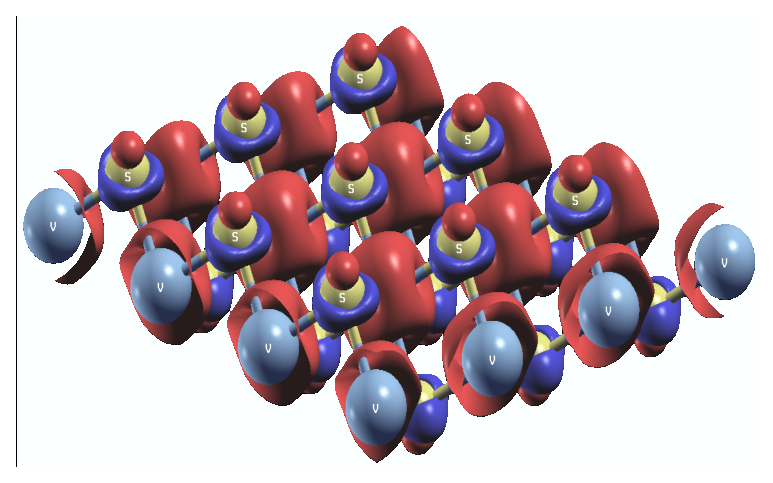
\epsfig{file=figRes/VS2/vs2magz.eps, scale=0.65}
 	\caption[Densidad de spin en el VS\textsubscript{2}.]{Distribuci\'on  de spin en el VS\textsubscript{2} en donde se muestra un valor de iso superficie de $\pm 0.002$, en donde el color rojo indica un valor positivo y el azul el negativo.}
 	\label{Sim:fig:distmagnVs2}
 \end{figure}
\section{An\'alisis de la introducci\'on de una vacancia de metal de transición } \label{Sim:sec:MdefVac}
A continuaci\'on se explica el comportamiento de la magnetizaci\'on por la introducci\'on de una vacancia del metal de transición en los materiales descritos anteriormente. El la sub secci\'on \ref{Sim:subsec:vacPt} se explica el efecto de la vacancia de Platino en PtSe\textsubscript{2} y PtS\textsubscript{2} y en la subsecci\'on \ref{Sim:subsec:vacV} se estudia el efecto de la vacancia de Vanadio en el VSe\textsubscript{2} y VS\textsubscript{2}.
\subsection{Vacancia de Platino en PtSe\textsubscript{2} y PtS\textsubscript{2}} \label{Sim:subsec:vacPt}
En la figura \ref{Sim:fig:supVac} se muestran las superceldas con la vacancia de platino en PtSe\textsubscript{2} y PtS\textsubscript{2}; se nota que los \'atomos de Selenio o Azufre que son vecinos al \'atomo faltante, indicado con lineas punteadas azules, se alejan entre si acerc\'andose a los \'atomos de Platino  vecinos. Este fen\'omeno debe a que los electrones que formaban parte de los enlaces covalentes con el \'atomo de platino quedan libres y aparece une gas de electrones en el lugar de la  vacancia. Para poder apreciar este efecto se muestra en la figura \ref{Sim:fig:cargavac}  la distribuci\'on de carga para valores positivos en escala logar\'itmica para las supercelda de PtSe\textsubscript{2} y  PtS\textsubscript{2}, se puede observar que existe una peque\~na distribuci\'on de electrones en el lugar del \'atomo faltante.

\begin{figure}[!hbt]
	\centering
	\subfigure[en PtSe\textsubscript{2}]{
		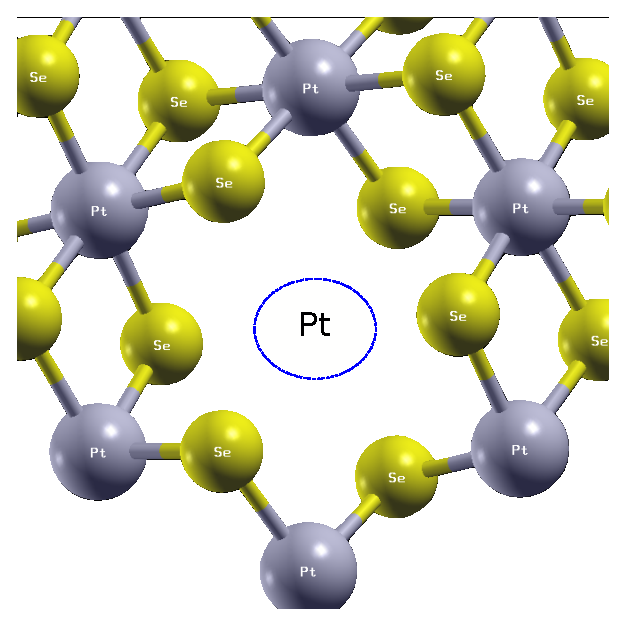
\epsfig{file=figRes/PtSe2/VacanciaPt.eps, scale=0.6}
	\label{Sim:fig:supVacptse2}
	}
    \subfigure[en PtS\textsubscript{2}]{
    	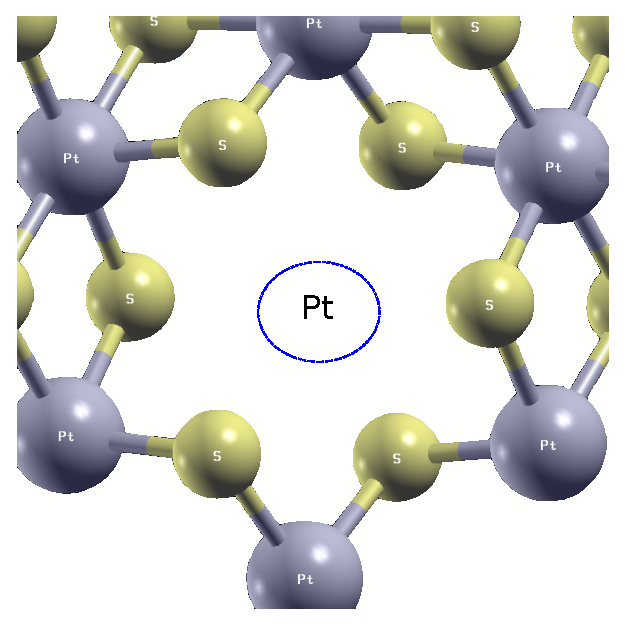
\epsfig{file=figRes/PtS2/VacanciaPt.eps, scale=0.6}
    	\label{Sim:fig:supVacpts2}
    }
    \caption[Superceldas de  PtSe\textsubscript{2} y PtS\textsubscript{2} con vacancia de Platino.]{Supercelda con vacancia de Platino en PtSe\textsubscript{2} (\ref{Sim:fig:supVacptse2}) y PtS\textsubscript{2} (\ref{Sim:fig:supVacpts2}).}
    \label{Sim:fig:supVac}
\end{figure}

\begin{figure}[!hbt]
	\centering
	\subfigure[PtSe\textsubscript{2}]{
		\includegraphics[scale=0.8]{figRes/PtSe2/densidades/densPos/densidadpos.pdf}
		\label{Sim:fig:cargavacPtse2}
	}
   \subfigure[PtS\textsubscript{2}]{
   	\includegraphics[scale=0.8]{figRes/PtS2/def/densidades/denspos/densidadpos.pdf}
   	\label{Sim:fig:cargavacPts2}
   }
  \caption[Distribuci\'on de carga en alrededor de la vacancia de platino en PtSe\textsubscript{2} y PtSe\textsubscript{2}.]{Distribuci\'on de carga alrededor de la vacancia de platino en PtSe\textsubscript{2} (\ref{Sim:fig:cargavacPtse2}), y en PtS\textsubscript{2} (\ref{Sim:fig:cargavacPtse2}).}
 \label{Sim:fig:cargavac}	
\end{figure}
%\newline
%\newline
En la figura \ref{Sim:fig:bandasSOCPtSe2vac} se muestra el diagrama de bandas con su densidad de estados,donde  se puede apreciar que el principal efecto que se observa es la aparici\'on de  dos niveles dentro de la banda prohibida y al aumento de la separaci\'on entre los dos \'ultimos niveles de la banda de valencia. Adicionalmente se puede notar que en la densidad de estados, los dos niveles dentro de la brecha prohibida provienen de los orbitales $p$ del \'atomo de Selenio vecino a la vacancia; mientras que el orbital $p$ de un \'atomo de selenio, que mantiene sus enlaces originales completos, no contribuye considerablemente a la creación de estos niveles. en relaci\'on a los orbitales $d$ del platino,  la casi igualdad que exist\'ia con los orbitales $p$ del Selenio en la banda de conducci\'on desaparece y ahora la mayor contribuci\'on viene de los orbitales de Selenio que no son vecinos de la vacancia.

\begin{figure}
	\centering
	\includegraphics[width=12cm, height=7cm]{figRes/PtSe2/def/bandas/comparacionbandas/bandasDOS.pdf}
	\caption[Diagrama de bandas y densidad de estados del PtSe\textsubscript{2} con vacancia de Platino y efecto spin-\'orbita.]{diagrama de bandas y la densidad de estados mostrando las contribuciones del orbital $d$ del Platino y $d$ del \'atomo de Selenio vecino del \'atomo faltante y otro que no lo es.}
	\label{Sim:fig:bandasSOCPtSe2vac}
\end{figure}

Mediante la introducci\'on de este defecto se observa que aparece un momento magn\'etico de $2.37~ \mu_{B}/celda$. En la figura \ref{Sim:fig:bandDefPtse2noSOC} se muestra el diagrama de bandas sin el efecto de spin-\'orbita y se puede observar que  las bandas con spin $\uparrow$ y $\downarrow$ se encuentran bien distribuidas y separadas;  adem\'as se tiene que las  bandas inducidas por efecto de la vacancia  dentro de la brecha prohibida   corresponden principalmente al  spin $\downarrow$  y de acuerdo  a la densidad de estados que se muestra a la izquierda del diagrama de bandas, \'estas est\'an formadas principalmente por electrones en el orbital $p$ de los \'atomos vecinos a la vacancia de Platino, sugiriendo   que estas  provienen de los electrones que quedan libres por los enlaces covalentes rotos. Adem\'as  se reporta la densidad de estados del orbital $p$ de un \'atomo de Selenio que no se ve afectado directamente por la vacancia,  donde que su distribuci\'on es muy similar a la observada en un material sin defectos, de tal forma que aporta una magnetizaci\'on de $0.003 ~\mu_{B}$.

\begin{figure}[!hbt]
	\centering
	\includegraphics[scale=0.9]{figRes/PtSe2/def/bandas/nosoc/bandasDOSnoSoc.pdf}
	\caption[Diagrama de bandas y densidad de estados del PtSe\textsubscript{2} con vacancia de Platino.]{Diagrama de bandas y densidad de estados sin incluir el efecto de spin \'orbita en el PtSe\textsubscript{2}, se muestran las bandas correspondientes a cada spin y en el caso de la densidad de estados se muestra las contribuciones del orbital $d$ del Platino y el $p$ del \'atomo de Selenio vecino de la vacancia y de un \'atomo que a\'un mantiene los tres enlaces covalentes.}
	\label{Sim:fig:bandDefPtse2noSOC}
\end{figure}

\begin{figure}[!hbt]
	\centering
	\includegraphics[scale=0.9]{figRes/PtSe2/def/bandas/nosoc/pdosS_neg.pdf}
	\caption[Densidad de estados proyectado en el orbital $p$ del \'atomo de Selenio en el PtSe\textsubscript{2} con vacancia de Platino.]{Densidad de estados del orbital $p$ del \'atomo de Selenio vecino de la vacancia de platino.}
	\label{Sim:fig:pdosSeptse2vac}
\end{figure} 

Para el orbital $p$ del \'atomo vecino a la vacancia de Platino,  se puede  observar en la figura \ref{Sim:fig:pdosSeptse2vac} que los estados generados dentro de la brecha prohibida provienen mayoritariamente de  los orbitales $p_z$ y $p_y$. Adem\'as, por debajo del nivel de Fermi (representado cono una l\'inea punteada en la figura \ref{Sim:fig:pdosSeptse2vac}) se puede observar que la diferencia en el n\'umero de estados con spin $\uparrow$ y $\downarrow$ para las tres componentes del orbital $p$ y la diferencia es mayor para los orbitales $p_x$ y $p_y$, por lo que se espera que el spin est\'e orientado en la direcci\'on del plano del sistema. Se tiene entonces un total una contribuci\'on al momento magn\'etico  de $0.224 ~\mu_{B}$. Para  la densidad de estados del orbital $d$ del Platino,  se  nota que la mayor contribuci\'on al momento magn\'etico proviene de los orbitales $d_{x^2-y^2}$ y $d_{xy}$ que est\'an orientados en la direcci\'on del plano del sistema y que tambi\'en presenta una contribuci\'on mas peque\~na de los orbitales $d_{zx}$ y $d_{zy}$, principalmente formando los estados de la banda de conducci\'on y en total el \'atomo de platino contribuye  con un momento magn\'etico de $0.03~ \mu_{B}$.

\begin{figure}[!hbt]
	\centering
	\includegraphics[scale=1]{figRes/PtSe2/def/bandas/nosoc/pdosPt_3.pdf}
	\caption[Densidad de estados proyectado del orbital $d$ del Platino en el PtSe\textsubscript{2} con vacancia de Platino.]{Densidad de estados del orbital $d$ del \'atomo de Platino.}
	\label{Sim:fig:pdosPtdtse2vac}
\end{figure}  
\par En el caso del PtS\textsubscript{2} se observan en la figura \ref{Sim:fig:VacPtsocPtS2} el diagrama de bandas con el efecto de spin-\'orbita y la densidad de estados con  el pDOS del orbital $d$ del \'atomo de Platino y el orbital $p$ de un \'atomo de Azufre vecino a la vacancia y  de uno que no lo es. Se observa que aparecen algunas bandas dentro de la brecha prohibida y las cuales son muy similares a las observadas en el PtSe\textsubscript{2}, aunque se observa que el nivel de Fermi se desplaza dentro de la banda de valencia y se ve que los estados dentro de la brecha prohibida provienen de los \'atomos de Azufre vecinos a la vacancia.
\begin{figure}[!hbt]
	\centering
	\includegraphics[width=12cm, height=7cm]{figRes/PtS2/def/bandas/soc/bandasDOS.pdf}
	\caption[Diagrama de bandas y densidad de estados incluyendo el efecto de spin-\'orbita en PtS\textsubscript{2} con una vacancia de Platino]{Diagrama de bandas y densidad de estados del PtS\textsubscript{2} con vacancia de Platino incluyendo el efecto de spin-\'orbita.}
	\label{Sim:fig:VacPtsocPtS2}
\end{figure}

En este caso aparece un momento magn\'etico de $2.63 ~ \mu_{B}/celda$. En la figura \ref{Sim:fig:noSOCpts2def} se muestra el diagrama de bandas indicando su distribuci\'on  para cada spin $\uparrow$ y $\downarrow$. N\'otese que las bandas que se generan por el efecto de la vacancia provienen del orbital $p$ del \'atomo de Azufre, cercano a la vacancia del Platino. De igual manera que con el PtSe\textsubscript{2} el \'atomo de Azufre que no se ve afectado por la vacancia, no muestra una magnetizaci\'on considerable; adem\'as de que la densidad de estados correspondiente al orbital $p$ de este \'atomo no es muy distinta al del sistema sin deformar.
\newline

\begin{figure}[!hbt]
	\centering
	\includegraphics[scale=0.9]{figRes/PtS2/def/bandas/nosoc/bandasDOSnoSoc.pdf}
	\caption[Diagrama de bandas y densidad de estados del PtS\textsubscript{2} con una vacancia de Platino.]{Diagrama de bandas y densidad de estados del PtS\textsubscript{2} en donde se muestra la distribuci\'on del spin, en el caso de la densidad de estados la densidad de estados total se multiplic\'o por 0.2 para una mejor visualizaci\'on.  }
	\label{Sim:fig:noSOCpts2def}
\end{figure}
Si se analiza la densidad de estados proyectada del \'atomo de Azufre, que a\'un conserva sus tres  enlaces,  ( fig.  \ref{Sim:fig:pdosSnovacpts2}),   se puede observar que si existe un peque\~no efecto que puede ser debido al esfuerzo que se induce con la creaci\'on de la vacancia, se puede notar que si contribuyen poco a la formaci\'on de los estados dentro de la brecha prohibida, aunque ya se nota que en los estados por debajo del nivel de Fermi existe una peque\~na diferencia en el n\'umero de estados con spin $\uparrow$ y $\downarrow$; de tal forma que tiene una contribuci\'on al momento magn\'etico de $0.01 ~\mu_{B}$.
\begin{figure}[!hbt]
	\centering
	\includegraphics[scale=1]{figRes/PtS2/def/bandas/nosoc/pdosS_ps.pdf}
	\caption[Densidad de estados proyectada en los orbitales $p$ del \'atomo de Azufre en el PtS\textsubscript{2} con una vacancia de Platino.]{Densidad de estados parcial de los orbitales $p$ del \'atomo de Azufre que no es vecino a la vacancia.}
	\label{Sim:fig:pdosSnovacpts2}
\end{figure}
%\newline
En la figura \ref{Sim:fig:pdosSvacpts2} se tiene la densidad de estados del orbital $p$ del \'atomo de Azufre vecino de la vacancia y se puede notar que la mayor contribuci\'on  a los niveles provocados por la vacancia proviene del orbital $p_y$. Dicho orbital tambi\'en contribuye a los estados cercanos al nivel de Fermi, lo cual es distinto a lo que sucede en el \'atomo de azufre que a\'un mantiene sus enlaces (fig. \ref{Sim:fig:pdosSnovacpts2}). En cuanto a la contribuci\'on de la magnetizaci\'on se puede observar que proviene principalmente de  los orbitales $p_x$ y $p_y$ lo que favorece a que los spines se orienten en estas direcciones, en total este \'atomo aporta una magnetizaci\'on de $0.283~ \mu_B$.
\begin{figure}[!hbt]
	\centering
	\includegraphics[scale=1]{figRes/PtS2/def/bandas/nosoc/pdosS_neg.pdf}
	\caption[Densidad de estados proyectada en los orbitales $p$ del \'atomo de Azufre vecino a la vacancia en el PtS\textsubscript{2} con una vacancia de Platino.]{Densidad de estados parcial de los orbitales $p$ del \'atomo de azufre vecino a la vacancia.}
	\label{Sim:fig:pdosSvacpts2}
\end{figure}
\newline
En el caso del \'atomo de platino, este  tambi\'en contribuye a la formaci\'on de los estados dentro de la brecha prohibida, tal como se muestra en la figura \ref{Sim:fig:pdosPtvacpts2} los orbitales $d_{x^2-y^2}$ y $d_{xy}$ son los principales componentes de estos estados. En general estos orbitales, junto con $d_{z^2}$,  contribuyen a la diferencia de poblaci\'on  para los spines $\uparrow$ y $\downarrow$ y  por lo tanto la contribuci\'on a la magnetizaci\'on es de $0.044 ~ \mu_B$. La aparici\'on de este efecto se debe a que los enlaces met\'alicos entre los \'atomos de platino se debilitan y de esta forma aparece una peque\~na magnetizaci\'on.

\begin{figure}[!hbt]
	\centering
	\includegraphics[scale=1]{figRes/PtS2/def/bandas/nosoc/pdosPt_3.pdf}
	\caption[Densidad de estados proyectada en los orbitales $d$ del \'atomo de Platino en el PtS\textsubscript{2} con una vacancia de Platino.]{Densidad de estados parcial de los orbitales $d$ del \'atomo de platino.}
	\label{Sim:fig:pdosPtvacpts2}
\end{figure}

En la figura \ref{Sim:fig:CargaVacPtse2} se muestra la distribuci\'on de carga en el PtSe\textsubscript{2} y se puede notar que en los \'atomos de Selenio que est\'an cercanos a la vacancia, los electrones se agrupan orient\'andose en hacia la vacancia,  indicando que los electrones no est\'an formando nuevos enlaces. Tambi\'en se puede notar que los orbitales $p_z$ y $p_y$ se est\'an  hibridizando. En la figura \ref{Sim:fig:MagzVacPtse2} se muestra la distribuci\'on de spines en el PtSe\textsubscript{2} lo cual refleja la magnetizaci\'on. Estos se encuentran mayormente localizados en el los \'atomos de Selenio cercanos a la vacancia,  concordando con lo observado en la densidad de estados (fig. \ref{Sim:fig:pdosSeptse2vac}).
\begin{figure}[!hbt]
	\centering
	\subfigure[densidad de carga]{
		\epsfig{file=figRes/PtSe2/def/ptse2_carga, scale=0.9}
		\label{Sim:fig:CargaVacPtse2}
	}
    \subfigure[densidad de spines]{
    	\epsfig{file=figRes/PtSe2/def/ptse2_magz, scale=0.9}
    	\label{Sim:fig:MagzVacPtse2}
    }
  \caption[Iso superficies de la densidad de carga y de spin en el PtSe\textsubscript{2} con vacancia de Platino.]{Isosuperficies de la densidad de carga (\ref{Sim:fig:CargaVacPtse2}) y la densidad de spines (\ref{Sim:fig:MagzVacPtse2} del PtSe\textsubscript{2} con un valor de $0.001 e/\AA^3$. }
\end{figure}


 En el caso del PtS\textsubscript{2}  se observa en la figura \ref{Sim:fig:CargaVacPts2}  la densidad de carga  cerca de la vacancia y es posible observar los enlaces covalentes entre los \'atomos de Platino y Azufre y en la regi\'on de la vacancia se observa que los orbitales $p_z$ y el $p_y$ se hibridizan tal como sucede con el  ptSe\textsubscript{2}. En cuanto la magnetizaci\'on se    tiene que la densidad de spines se concentra en los \'atomos cercanos a la vacancia, debido a que los electrones no se encuentran formando enlaces y se puede notar que dicha distribuci\'on es la esperada en acuerdo a la densidad parcial de estados para el azufre (fig. \ref{Sim:fig:pdosSvacpts2}).
 \begin{figure}[!hbt]
 	\centering
 	\subfigure[densidad de carga]{
 		\epsfig{file=figRes/PtS2/def/densidades/pts2_carga, scale=0.9}
 		\label{Sim:fig:CargaVacPts2}
 	}
 	\subfigure[densidad de spines]{
 		\epsfig{file=figRes/PtS2/def/densidades/pts2_magz, scale=0.9}
 		\label{Sim:fig:MagzVacPts2}
 	}
 	\caption[Iso superficies de la densidad de carga y de spin en el PtS\textsubscript{2} con vacancia de Platino.]{Isosuperficies de la densidad de carga (\ref{Sim:fig:CargaVacPts2}) y la densidad de spines (\ref{Sim:fig:MagzVacPts2} del PtS\textsubscript{2} con un valor de $0.001 e/\AA^3$. }
 \end{figure}     
\subsection{Vacancia de Vanadio en VSe\textsubscript{2} y VS\textsubscript{2}} \label{Sim:subsec:vacV}
Es importante analizar esta clase de defectos debido a que se observa un fen\'omeno distinto a los materiales con Platino, ya que en lugar de que los \'atomos de Selenio y Azufre, se alejen entre  si estos se acercan. En la figura \ref{Sim:fig:vacV} se detallan las superceldas con la vacancia de Vanadio con las posiciones de los \'atomos ya optimizadas.
\newline
\begin{figure}[!hbt]
	\centering
	\subfigure[VSe\textsubscript{2}]{
		\epsfig{file=figRes/VSe2/def/vacVse2_def, scale=0.7}
		\label{Sim:fig:vacVvse2}
	}
    \subfigure[VS\textsubscript{2}]{
    	\epsfig{file=figRes/VS2/def/vs2_def, scale=0.7}
    	\label{Sim:fig:vacVvs2}
    }
  \caption[Superceldas de VSe\textsubscript{2} y VS\textsubscript{2} con vacancia de vanadio.]{Superceldas con la vacancia de Vanadio. Visualizada con XcrySDen.}
  \label{Sim:fig:vacV}
\end{figure}

En la figura \ref{Sim:fig:cargavacV} se muestra la distribuci\'on de carga en la regi\'on de la vacancia en el VSe\textsubscript{2} y VS\textsubscript{2}, en donde se puede observar que no existe distribuci\'on de carga en la posici\'on en donde se ubicaba el \'atomo de Vanadio, lo cual explica el motivo por el cual no se separan los \'atomos  vecinos de la vacancia tal como sucede con el PtSe\textsubscript{2} y PtS\textsubscript{2}.
\newline
\begin{figure}[!hbt]
	\centering
	\subfigure[VSe\textsubscript{2}]{
		\epsfig{file=figRes/VSe2/def/densidad/densPos/densidadpos, scale=0.9}
		\label{Sim:fig:cargavacVSe2}
	}
	\subfigure[VS\textsubscript{2}]{
		\epsfig{file=figRes/VS2/def/dens/densPos/densidadpos, scale=0.9}
		\label{Sim:fig:cargavacVS2}
	}
\caption[Densidad de carga en el VSe\textsubscript{2} yVS\textsubscript{2}]{densidad de carga en la regi\'on de la vacancia en el VSe\textsubscript{2} y VS\textsubscript{2} visualizada con XcrySDen }
\label{Sim:fig:cargavacV}	
\end{figure}
%\newline
\begin{figure}[!hbt]
	\centering
	\includegraphics[scale=1]{figRes/VSe2/def/bandas/soc/bandasDOS.pdf}
	\caption[Diagrama de bandas y densidad de estados con el efecto spin-\'orbita del VSe\textsubscript{2} con vacancia de Vanadio.]{Estructura de bandas y densidad de estados de la supercelda de Vse\textsubscript{2} con un vacancia de vanadio y el efecto de spin-\'orbita.}
	\label{Sim:fig:vacVvse2band}
\end{figure}
%\newline
\par En la figura \ref{Sim:fig:vacVvse2band} se muestra el diagrama de bandas y la densidad de estados  del  VSe\textsubscript{2}. En cuanto a la densidad de estados se observa que mantiene  una forma muy similar al caso de la estructura sin defectos (fig. \ref{Sim:fig:bandSocVSe2}). En cuanto al diagrama de bandas  se observan mas bandas que en el caso que se estudi\'o en la sub secci\'on \ref{Sim:subsec:vse2cU} y esto es debido a que las estructuras tienen mas \'atomos que en el caso de la celda unitaria y no necesariamente se deben a la vacancia, en la figura \ref{Sim:fig:bandasvse2orb} se observa la distribuci\'on de los orbitales en el espacio rec\'iproco y se puede notar que los orbitales $p$ del \'atomo de selenio vecino ala vacancia se encuentran localizados en ciertas posiciones cercanas al nivel de Fermi. 
\begin{figure}[!hbt] 
	\centering
	\includegraphics[scale=1]{figRes/VSe2/def/bandas/soc/bandasSe.pdf}
	\caption[Distribuci\'on de los orbitales de los \'atomos en el diagrama de bandas del VSe\textsubscript{2} con vacancia de Vanadio.]{Distribuci\'on de los orbitales $p$ del \'atomo de Selenio y $d$ del Vanadio.}
	\label{Sim:fig:bandasvse2orb}
\end{figure}
\newline
\par En la figura \ref{Sim:fig:VSe2noSOCcavband} se muestra el diagrama de bandas indicando a qu\'e spin pertenecen, not\'andose ahora la diferencia de poblaci\'on entre los electrones de spin $\uparrow$ y $\downarrow$ provocando una magnetizaci\'on de $0.48 ~\mu_{B}/ celda$. Si se compara la magnetizaci\'on de la supercelda sin defectos que es $3.19~\mu_{B}/celda$, se nota que se reduce la magnetizaci\'on considerablemente y para poder explicar la raz\'on de este fen\'omeno, es necesario observar los cambios en las contribuciones de los \'atomos del sistema a la magnetizaci\'on total. 
\begin{figure}[!hbt]
	\centering
	\includegraphics[width=13cm, height=9cm]{figRes/VSe2/def/bandas/nosoc/bandasDOSnoSoc.pdf}
	\caption[Diagrama de bandas y densidad de estados del VSe\textsubscript{2} con vacancia de Vanadio.]{Diagrama de bandas y la densidad de estados para los spin $\uparrow$ y $\downarrow$ mostrando la distribuci\'on de estos} 
	\label{Sim:fig:VSe2noSOCcavband}
\end{figure}
%\newline
\par Analizando el comportamiento de los \'atomos de Selenio que no es vecino de la vacancia, se observa que  no se ve afectado directamente por la vacancia, ya que presenta una magnetizaci\'on de $-0.012~\mu_{B}$, la cual es menor que en el caso expuesto en la subsecci\'on \ref{Sim:subsec:vse2cU}. En la figura \ref{Sim:fig:pdosSeVse2} se observa la densidad de estados de los orbitales $p$ del \'atomo de Selenio con sus enlaces completos y es posible apreciar que la mayor\'ia de los estados provienen de los orbitales $p_y$ y $p_z$ y al igual que en el caso sin defectos, existe una regi\'on entre el nivel de Fermi y 0.5 eV por encima de este, en donde no existe una gran contribuci\'on de estados. Para el caso de la densidad de estados del \'atomo vecino  a la vacancia de vanadio (fig. \ref{Sim:fig:pdosSevacVse2}), se puede observar que en la regi\'on pr\'oxima al nivel de Fermi, s\'i existen mas estados que provienen de los orbitales $p_y$ y $p_z$ y, a diferencia de los materiales con Platino, no aumenta la contribuci\'on en la magnetizaci\'on, ya que aportan $-0.007~ \mu_{B}$, por  lo que pr\'acticamente no aportan a la magnetizaci\'on total del sistema. En principio esto no reducir\'ia la magnetizaci\'on del material debido a que en el caso del VSe\textsubscript{2}, la mayor contribuci\'on proviene de los \'atomos de Vanadio.
%\newline
 
\begin{figure}[!hbt]
	\centering
	\includegraphics[scale=1]{figRes/VSe2/def/bandas/nosoc/pdosSe.pdf}
	\caption[Densidad de estados parcial de los orbitales $p$ del \'atomo de Selenio en VSe\textsubscript{2} con vacancia de vanadio]{Densidad de estados parcial de los orbitales $p$ del \'atomo de Selenio con enlaces completos.}
	\label{Sim:fig:pdosSeVse2}
\end{figure}

\begin{figure}[!hbt]
	\centering
	\includegraphics[scale=1]{figRes/VSe2/def/bandas/nosoc/pdosSe_vac.pdf}
	\caption[Densidad de estados parcial de los orbitales $p$ del \'atomo de Selenio vecino a la vacancia en VSe\textsubscript{2} con vacancia de vanadio]{Densidad de estados parcial de los orbitales $p$ del \'atomo de Selenio vecino a la vacancia.}
	\label{Sim:fig:pdosSevacVse2}
\end{figure}
En la figura \ref{Sim:fig:pdosVVse2} se puede  que la distribuci\'on de los orbitales $d_{x^2-y^2}$ y $d_{xy}$ son los que contribuyen mayoritariamente a la densidad de estados en la regi\'on cercana al nivel de Fermi y en los estados de mayor energ\'ia. En la regi\'on mas cercana al n\'ucleo la mayor contribuci\'on proviene de los orbitales $d_{zx}$ y $d_{zy}$; sin embargo, la diferencia de poblaciones proviene principalmente de los orbitales $d_{x^2-y^2}$ y $d_{xy}$ y por lo tanto, los spines siguen teniendo la misma orientaci\'on que en el caso del material sin defectos, pero la magnetizaci\'on se reduce a $0.16~\mu_B$, el cual es un valor 74\% menor al caso del material sin defectos.
\begin{figure}[!hbt]
	\centering
	\includegraphics[scale=1]{figRes/VSe2/def/bandas/nosoc/pdosV.pdf}
	\caption[Densidad de estados parcial de los orbitales $d$ del \'atomo de vanadio en VSe\textsubscript{2} con vacancia de vanadio]{Densidad de estados parcial de los orbitales $d$ del \'atomo de Vanadio.}
	\label{Sim:fig:pdosVVse2}
\end{figure} 
\newline
\begin{figure}[!hbt]
	\centering
	\includegraphics[scale=1]{figRes/VS2/def/bandas/nosoc/bandasSe.pdf}
	\caption[Distribuci\'on de los orbitales de los \'atomos en el diagrama de bandas del VS\textsubscript{2} con vacancia de Vanadio]{Distribuci\'on de los orbitales $p$ y $d$ de Azufre y vanadio en el diagrama de bandas}
	\label{Sim:fig:orbVacVS2bandas}
\end{figure}
\begin{figure}[!hbt]
	\centering
	\includegraphics[scale=1]{figRes/VS2/def/bandas/nosoc/bandasDOSnoSoc.pdf}
	\caption[Diagrama de bandas  y densidad de estados en el VS\textsubscript{2} con vacancia de Vanadio]{Diagrama de bandas y Densidad de Estados del  VS\textsubscript{2}.}
	\label{Sim:fig:VacVS2bandas}
\end{figure}
\par En el caso del VS\textsubscript{2} se tiene un fen\'omeno similar, tal como se observa en la figura \ref{Sim:fig:orbVacVS2bandas} el efecto de la vacancia de Vanadio induce que  ciertas bandas provengan de electrones del \'atomo de azufre cercano a la vacancia y estas se encuentran en posiciones cercanas al nivel de Fermi. dicha distribuci\'on se ve muy similar al del VSe\textsubscript{2}. En la figura \ref{Sim:fig:VacVS2bandas} se muestra el diagrama de bandas correspondiente a a cada spin ($\uparrow,~ \downarrow$) en donde se puede notar que existen bandas bien definidas  para cada spin por debajo del nivel de Fermi y por encima de este, tambi\'en se observa que las bandas para cada spin no son muy distintas. En cuanto a la densidad de estados se puede observar  que las mayores contribuciones provienen del orbital $d$ del Vanadio, aunque la diferencia entre estos y los provenientes del orbital $p$ del Azufre, ya no es tan grande como en el caso del material sin defectos (subsec. \ref{Sim:subsec:VS2}). Adem\'as de que se observa que la diferencia de poblaci\'on entre diferente spin es mas peque\~na que en el caso del material sin deformar, lo cual induce  una magnetizaci\'on de $0.76 ~\mu_B/celda$ y, si se compara con el valor $2.04 ~\mu_B/celda$  que se obtuvo con la supercelda sin defectos, se observa un valor menor. En cuanto el \'atomo de Vanadio en la figura \ref{Sim:fig:pdosVvacVS2} se muestra la densidad de estados parcial de los orbitales $d$ del \'atomo de Vanadio y se observa que la mayor diferencia de poblaci\'on entre los spines $\uparrow$ y $\downarrow$ proviene de los orbitales $d_{zx}$ y $d_{zy}$ en la regi\'on mas cercana al n\'ucleo y de los orbitales $d_{x^2-y^2}$ y $d_{xy}$ en la regi\'on cercana al nivel de Fermi y por lo tanto, la magnetizaci\'on se debe principalmente a la diferencia de poblaci\'on  de estos orbitales y cuyo valor es de $0.215~\mu_{B}$, el cual es un valor menor al que se obtuvo en el material sin defectos.
\begin{figure}[!hbt]
	\centering
	\includegraphics[scale=1]{figRes/VS2/def/bandas/nosoc/pdosV.pdf}
	\caption[Densidad de estados proyectada en los orbitales $d$ del Vanadio en VS\textsubscript{2} con vacancia de Vanadio.]{Densidad de estados parcial de los orbitales $d$ del \'atomo de Vanadio}
	\label{Sim:fig:pdosVvacVS2}
\end{figure}
%\newline
En cuanto  al \'atomo de Azufre, que aun tiene sus tres enlaces, se puede notar en la densidad de estados (fig. \ref{Sim:fig:pdosSVS2}) que la mayor contribuci\'on proviene del orbital $p_x$ en la regi\'on cercana al nivel de Fermi. Es posible notar que la diferencia de la poblaci\'on de spines no es muy grande y por lo tanto, se tiene una magnetizaci\'on de $-0.0092~\mu_B$. Para el \'atomo de azufre cercano a la vacancia se observa en la densidad de estados proyectada (fig. \ref{Sim:fig:pdosSvacVS2}) se puede notar que la mayor contribuci\'on proviene de los orbitales $p_y$ y $p_z$ en la regi\'on cercana al nivel de Fermi. Esto se puede deber a que los orbitales que participaban en los enlaces con el \'atomo de Vanadio se combinan con los orbitales $p_z$;  adem\'as se puede observar que si existen estados por encima del nivel de Fermi, que al igual que en el VSe\textsubscript{2}, se relacionan con estados generados con la vacancia y concuerda con lo observado en la distribuci\'on de los estados de los orbitales en le diagrama de bandas. En cuanto a la diferencia de las poblaciones de spines, esta proviene de estos dos orbitales y se tiene una magnetizaci\'on de   $-0.0038~\mu_{B}$, el cual es un valor peque\~no y se observa el mismo fen\'omeno que en el caso del VSe\textsubscript{2}, en donde la aportaci\'on de los \'atomos calc\'ogenos no contribuyen de la misma manera que en el material sin defectos.
\begin{figure}[!hbt]
	\centering
	\includegraphics[scale=1]{figRes/VS2/def/bandas/nosoc/pdosSe.pdf}
	\caption[Densidad de estados proyectada en los orbitales $p$ del Azufre en VS\textsubscript{2} con vacancia de Vanadio]{Densidad de estados parcial de los orbitales $P$ del \'atomo de Azufre que no se ve afectado por la vacancia de Azufre.}
	\label{Sim:fig:pdosSVS2}
\end{figure}
%\newline

 
\begin{figure}[!hbt]
	\centering
	\includegraphics[scale=1]{figRes/VS2/def/bandas/nosoc/pdosSe_vac.pdf}
	\caption[Densidad de estados proyectada en los orbitales $p$ del Azufre vecino de la vacancia en VS\textsubscript{2} con vacancia de Vanadio]{Densidad de estados parcial de los orbitales $p$ del \'atomo de Azufre vecino de la vacancia.}
	\label{Sim:fig:pdosSvacVS2}
\end{figure}

\par En la figura \ref{Sim:fig:cargaVac} se muestra la densidad de carga del VSe\textsubscript{2} (fig. \ref{Sim:fig:cargaVacVSe2}) y VS\textsubscript{2} (fig. \ref{Sim:fig:cargaVacVS2}), donde  se puede observar que los enlaces entre el calcogenuro y el Vanadio es covalente y que los \'atomos de Azufre y Selenio, que son cercanos a la vacancia de Vanadio, se comportan de la misma manera que los materiales con Platino. Es posible notar que los orbitales $p_z$ y $p_y$ se combinan y se puede notar en la parte inferior de la figura, que el \'atomo que no se ve afectado por la vacancia se conservan sus tres enlaces. 
\begin{figure}[!hbt]
	\centering
	\subfigure[VSe\textsubscript{2}]{
		\epsfig{file=figRes/VSe2/def/densidad/vse2_carga_vac.eps, scale=0.8}
		\label{Sim:fig:cargaVacVSe2}
	}
    \subfigure[VS\textsubscript{2}]{
    	\epsfig{file=figRes/VS2/def/dens/vs2_carga_vac.eps, scale=0.8}
    	\label{Sim:fig:cargaVacVS2}
    	
    }
  \caption[Densidad de electrones en el VSe\textsubscript{2} y VS\textsubscript{2} con vacancia de Vanadio.]{Iso superficies de la densidad de carga con  un valor de $\pm 0.001 e/\AA^3$}
  \label{Sim:fig:cargaVac}
\end{figure}
\newline
En relaci\'on a la densidad de spines (fig. \ref{Sim:fig:magzVacV}) se puede observar que los \'atomos cercanos en la vacancia no aportan una gran cantidad  a la densidad total y lo cual est\'a de acuerdo con lo observado en las densidades de estados de los \'atomos de Azufre y Selenio. 
\begin{figure}[!hbt]
	\centering
	\subfigure[VSe\textsubscript{2}]{
		\epsfig{file=figRes/VSe2/def/densidad/vse2_magz.eps, scale=0.8}
		\label{Sim:fig:magnVacVSe2}
	}
	\subfigure[VS\textsubscript{2}]{
		\epsfig{file=figRes/VS2/def/dens/vs2_magz.eps, scale=0.8}
		\label{Sim:fig:magnVacVS2}
		
	}
\caption[Densidad de spin en el VSe\textsubscript{2} y VS\textsubscript{2} con vacancia de Vanadio.]{Iso superficies de la densidad de spines con  un valor de $\pm 0.0002 e/\AA^3$}
\label{Sim:fig:magzVacV}
\end{figure}
\section{Estudio del efecto de las deformaciones en la magnetizaci\'on} \label{Sim:sec:Str}
\subsection{Efecto en VSe\textsubscript{2} y VS\textsubscript{2}}
Si se aplica una deformaci\'on mec\'anica isotr\'opica descrita en la Figura \ref{Met:fig:strainiso} y cuya magnitud de deformaci\'on se describe por la ecuaci\'on \ref{Met:ec:strain}, se puede observar que la variaci\'on de la magnetizaci\'on en el VSe\textsubscript{2} (fig. \ref{Sim:fig:strVSe2Iso}) y Vs\textsubscript{2} (fig. \ref{Sim:fig:strVS2Iso}) presentan  un comportamiento casi lineal con respecto a la variaci\'on de la deformaci\'on con  un valor que va desde $-0.05$ a $+0.05$; para el  VSe\textsubscript{2} la magnetizaci\'on cambia de $0.3$ a $1.04 ~\mu_B/celda$,  indicando un cambio en la magnetizaci\'on de $0.74~\mu_{B}/celda$. En el caso del VS\textsubscript{2} la variaci\'on de la magnetizaci\'on es de $0.23$ a $1 ~ \mu_{B}/celda$, lo cual indica un cambio   de  $0.77~\mu_{B}/celda$, sugiriendo un cambio mayor que en comparaci\'on con el VSe\textsubscript{2}. De igual forma se muestran im\'agenes de las estructuras deformadas con  valores de deformaci\'on  $\varepsilon= -0.05,~0.0,~0.05$. 

\begin{figure}[!hbt]
	\centering
	\subfigure[VSe\textsubscript{2}]{
		\includegraphics[scale=1.1]{figRes/VSe2/str/isotropico/magn.pdf}
		\label{Sim:fig:strVSe2Iso}
	}
    \subfigure[VS\textsubscript{2}]{
    	\includegraphics[scale=1.1]{figRes/VS2/str/isotropico/magn.pdf}
    	\label{Sim:fig:strVS2Iso}
    }
\caption[Magnetizaci\'on del VSe\textsubscript{2} y VS\textsubscript{2} en funci\'on de una deformaci\'on isotr\'opica. ]{Gr\'aficas de la magnetizaci\'on en funci\'on de la deformaci\'on isotr\'opica en VSe\textsubscript{2} y VS\textsubscript{2} mostrando el ajuste lineal de los datos.}
\label{Sim:fig:MgnVx2Iso}
\end{figure}

 Para poder analizar  la variaci\'on de la magnetizaci\'on se consideran los cambios en las distancias entre los distintos \'atomos que est\'an identificadas de acuerdo con lo que se muestra en la figura \ref{Sim:fig:disVX2Iso}. 
 \begin{figure}[!hbt]
 	\centering
 	\epsfig{file=figRes/compIso,scale=0.8}
 	\caption[ Distancias entre \'atomos   VSe\textsubscript{2} y VS\textsubscript{2} utilizados para el estudio de una deformaci\'on isotr\'opica]{Distancias entre \'atomos en el VSe\textsubscript{2} y  VS\textsubscript{2} en donde las esferas grises representran el vanadio y las amarillas El Azufre o Selenio.}
 	\label{Sim:fig:disVX2Iso}
 \end{figure}
\par Si se toma en cuenta el cambio de la distancia entre los dos \'atomos calc\'ogenos, es posible observar que el cambio correspondiente disminuye conforme aumenta la deformación tal y como se aprecia en la figura \ref{Sim:fig:DSVx2Iso} para en Vse\textsubscript{2} y VS\textsubscript{2}. En este caso no se observa  una tendencia parecida a la magnetizaci\'on. En cuanto a la distancia entre el \'atomo de Vanadio y el Azufre  o Selenio, se muestra en la figura \ref{Sim:fig:DVSVx2Iso} la  variaci\'on del cambio de la distancia entre estos dos \'atomos y es posible notar que se comportan de forma lineal y con una tendencia similar a la magnetizaci\'on. En esta figura se muestran adem\'as las lineas de dicha  tendencia y se puede notar que el cambio es mayor en el caso del VS\textsubscript{2}, lo cual  concuerda con lo observado en la magnetización. 

\begin{figure}[!hbt]
	\centering
	\subfigure[VSe\textsubscript{2}]{
		\includegraphics[scale=1]{figRes/VSe2/str/isotropico/dS.pdf}
		\label{Sim:fig:DSVSe2Iso}
	}
	\subfigure[VS\textsubscript{2}]{
		\includegraphics[scale=1]{figRes/VS2/str/isotropico/dS.pdf}
		\label{Sim:fig:DSVS2Iso}
	}
	\caption[Cambio en la distancia entre \'atomos de Selenio o Azufre  y Vanadio en  VSe\textsubscript{2} y VS\textsubscript{2} en funci\'on de una deformaci\'on isotr\'opica]{Cambio en la distancia entre dos \'atomos de Selenio en VSe\textsubscript{2} y Azufre en VS\textsubscript{2}.}
	\label{Sim:fig:DSVx2Iso}
\end{figure}
\begin{figure}[!hbt]
	\centering
	\subfigure[VSe\textsubscript{2}]{
		\includegraphics[scale=1]{figRes/VSe2/str/isotropico/dVS.pdf}
		\label{Sim:fig:DVSVSe2Iso}
	}
	\subfigure[VS\textsubscript{2}]{
		\includegraphics[scale=1]{figRes/VS2/str/isotropico/dVS.pdf}
		\label{Sim:fig:DVSVS2Iso}
	}
	\caption[Cambio en la distancia entre \'atomos de Selenio o Azufre en  VSe\textsubscript{2} y VS\textsubscript{2} en funci\'on de una deformaci\'on isotr\'opica. ]{Cambio en la distancia entre dos \'atomos de Selenio en VSe\textsubscript{2} y Azufre en VS\textsubscript{2}.}
	\label{Sim:fig:DVSVx2Iso}
\end{figure}
\par Para la deformaci\'on anisotr\'opica que se muestra en la figura \ref{Met:fig:strainanis} se observa  en la figura \ref{Sim:fig:MgnVx2Anis} la magnetizaci\'on en funci\'on de la deformaci\'on $\varepsilon_x$  y es posible notar que no existen cambios considerables  de tal forma que se puede argumentar que se mantiene constante; el principal efecto de aplicar dicha deformaci\'on es que ya no existe un \'angulo de $120 \degree$ entre los \'atomos de Vanadio y esto provoca que se pierda la simetr\'ia octaedral; sin embargo, las estructuras no sufren grandes cambios tal y como se puede notar en las figuras \ref{Sim:fig:strVSe2anis} y \ref{Sim:fig:strVS2Anis}.
\begin{figure}[!hbt]
	\centering
	\subfigure[VSe\textsubscript{2}]{
		\includegraphics[scale=1.15]{figRes/VSe2/str/anisotropico/magn.pdf}
		\label{Sim:fig:strVSe2anis}
	}
	\subfigure[VS\textsubscript{2}]{
		\includegraphics[scale=1.15]{figRes/VS2/str/anisotropico/magn.pdf}
		\label{Sim:fig:strVS2Anis}
	}
	\caption[Magnetizaci\'on del VSe\textsubscript{2} y VS\textsubscript{2} bajo una deformaci\'on anisotr\'opica.]{Gr\'aficas de la magnetizaci\'on en funci\'on de la deformaci\'on anisotr\'opica en VSe\textsubscript{2} y VS\textsubscript{2}.}
	\label{Sim:fig:MgnVx2Anis}
\end{figure}
Dicha deformaci\'on provoca que la distancia entre los \'atomos de Azufre o Selenio y Vanadio  sea diferente para cada \'atomo de Vanadio  vecino. En el caso de esta deformaci\'on las dos distancias se siguen comportando de la misma manera y una no, estas dos distancias con comportamientos diferentes se encuentran marcadas por $(S,Se-V)_{1,2}$ en la figura \ref{Sim:fig:disVX2Anis}. De igual forma la distancia entre calc\'ogenos no es la misma y est\'an indicadas por $(S,Se-S,Se)_{1,2}$. 
\begin{figure}[!hbt]
	\centering
	\epsfig{file=figRes/compAnis.eps,scale=0.9}
	\caption[Distancias entre \'atomos   VSe\textsubscript{2} y VS\textsubscript{2} utilizados para el estudio de una deformaci\'on anisotr\'opica.]{Distancias entre \'atomos en el VSe\textsubscript{2} y  VS\textsubscript{2} en la deformaci\'on anisotr\'opica, las esferas grises representan el vanadio y las amarillas El Azufre o Selenio.}
	\label{Sim:fig:disVX2Anis}
\end{figure}
%\newline
Esta 'ultima deformaci\'on se aplic\'o para valores de $\varepsilon_x$ de $-0.03$ a $0.03$, lo que indujo un cambio en el \'angulo entre los \'atomos de Vanadio  de $\pm 3 \degree$ en ambos materiales. Sin embargo no provoca grandes cambios en la distancia entre los \'atomos de vanadio tal y como se observa en la figura \ref{Sim:fig:compdV}  donde se puede notar que el cambio en la deformaci\'on anisotr\'opica es mas peque\~no. Al momento de observar el cambio de las distancias $(S,Se-S,Se)_{1,2}$ que se muestran en la figura \ref{Sim:fig:compdSSVX2}, es posible notar que en el caso del VSe\textsubscript{2}  la variaci\'on de las correspondientes distancias tienen signos contrarios; es decir, que mientras $\Delta (Se-Se)_{1}$  aumenta con el incremento de $\varepsilon_x$,  $\Delta (Se-Se)_{2}$ disminuye. Si se calcula la variaci\'on promedio (que se muestra en la figura \ref{Sim:fig:compdSSeVse2}) se nota que ronda entre $\pm 0.01 \AA$. En el caso del VS\textsubscript{2} (fig. \ref{Sim:fig:compdSSVs2}) los cambios en la variaci\'on de $\Delta (S-S)_{1,2}$  se comportan de la misma manera que en el  VSe\textsubscript{2}. Como se puede notar en  ambos casos el cambio es considerable.
\begin{figure}[!hbt]
	\centering
	\subfigure[VSe\textsubscript{2}]{
		\includegraphics[scale=0.8]{figRes/VSe2/str/com/CompdPt.pdf}
		\label{Sim:fig:compdVVse2}	
	}
	\subfigure[VS\textsubscript{2}]{
		\includegraphics[scale=0.8]{figRes/VS2/str/com/CompdPt.pdf}
	  \label{Sim:fig:compdVVs2}	
	}
	
	\caption[Comparaci\'on del cambio en la distancia entre los \'atomos de Platino por una deformaci\'on isotr\'opica y anisotr\'opica]{Comparaci\'on del cambio en da distancia entre \'atomos de vanadio bajo una deformaci\'on isotr\'opica y otra anisotr\'opica.}
	\label{Sim:fig:compdV}
\end{figure}

\begin{figure}[!hbt]
	\centering
	\subfigure[VSe\textsubscript{2}]{
		\includegraphics[scale=1.1]{figRes/VSe2/str/anisotropico/CompdSS.pdf}
		\label{Sim:fig:compdSSeVse2}	
	}
	\subfigure[VS\textsubscript{2}]{
		\includegraphics[scale=1.1]{figRes/VS2/str/anisotropico/CompdSS.pdf}
		\label{Sim:fig:compdSSVs2}	
	}
 \caption[Variaci\'on de la distancia entre \'atomos de Selenio y Azufre en VSe\textsubscript{2} y VS\textsubscript{2} mediante una deformaci\'on anisotr\'opica]{variaci\'on de las distancias entre \'atomos de Selenio en el VSe\textsubscript{2} y de Azufre en VS\textsubscript{2}.}
 \label{Sim:fig:compdSSVX2}
\end{figure}
%\newline
\par En la figura \ref{Sim:fig:compdSVVX2} se muestra la variaci\'on de la distancia entre el Selenio o Azufre  y el Vanadio, donde se puede observar un comportamiento muy similar al  caso de las distancias entre \'atomos de Azufre o Selenio descritos anteriormente y en la figura \ref{Sim:fig:compdSVVse2} se indica el cambio $\Delta (Se-V)_{1,2}$, en donde se tiene que, es posible observar que  mientras  $\Delta (Se-V)_{1}$ aumenta con el incremento de $\varepsilon_x$, $\Delta (Se-V)_{2}$ disminuye. El cambio promedio de $\Delta (Se-V)$ da un valor que var\'ia entre $-0.004$ y $0.007 ~\AA$.  Para el VS\textsubscript{2} (fig. \ref{Sim:fig:compdSVVs2})
sucede el mismo comportamiento  en donde es posible observar un cambio promedio que se encuentra entre el mismo rango que en el VSe\textsubscript{2}.
\begin{figure}[!hbt]
	\centering
	\subfigure[VSe\textsubscript{2}]{
		\includegraphics[scale=1]{figRes/VSe2/str/anisotropico/CompdVS.pdf}
		\label{Sim:fig:compdSVVse2}	
	}
	\subfigure[VS\textsubscript{2}]{
		\includegraphics[scale=1]{figRes/VS2/str/anisotropico/CompdVS.pdf}
		\label{Sim:fig:compdSVVs2}	
	}
	\caption[Variaci\'on de la distancia entre los \'atomos calc\'ogenos y el \'atomo de vanadio  (VSe\textsubscript{2} y VS\textsubscript{2})bajo una deformaci\'on anisotr\'opica]{variaci\'on de las distancias entre \'atomos de Selenio en el VSe\textsubscript{2} y de Azufre en VS\textsubscript{2}.}
	\label{Sim:fig:compdSVVX2}
\end{figure}
%\newline
\par Dado que el cambio en la distancia entre los \'atomos de Selenio o Azufre  y el \'atomo de Vanadio es muy peque\~no, entonces la interacci\'on entre estos dos \'atomos no var\'ia considerablemente causando que la magnetizaci\'on individual de estos \'atomos pr\'acticamente no cambia tal y como se muestra en la figura \ref{Sim:fig:cmagVX2}. 
\begin{figure}[!hbt]
	\centering
	\subfigure[VSe\textsubscript{2}]{
		\includegraphics[scale=1.1]{figRes/VSe2/str/anisotropico/CompMag.pdf}
		\label{Sim:fig:cmagVse2}	
	}
	\subfigure[VS\textsubscript{2}]{
		\includegraphics[scale=1.1]{figRes/VS2/str/anisotropico/CompMag.pdf}
		\label{Sim:fig:cmagVs2}	
	}
	\caption[Magnetizaci\'on de los \'atomos individuales en el VS\textsubscript{2} y VSe\textsubscript{2} bajo una deformaci\'on anisotr\'opica]{Magnetizaci\'on del \'atomo de vanadio y selenio o Azufre en el VSe\textsubscript{2} (\ref{Sim:fig:cmagVse2}) y VS\textsubscript{2} (\ref{Sim:fig:cmagVs2}) bajo una deformaci\'on anisotr\'opica.}
	\label{Sim:fig:cmagVX2}
\end{figure}
%\newline
\par En el caso de la deformaci\'on isotr\'opica se observa un fen\'omeno diferente: en la figura \ref{Sim:fig:cmagVX2I} es posible notar que la magnetizaci\'on del \'atomo de Vanadio se comporta de la misma manera que la magnetizaci\'on de todo el sistema (fig. \ref{Sim:fig:MgnVx2Iso}) y en ambos caso se observa un comportamiento muy similar de la magnetizaci\'on del \'atomo de Vanadio para  VSe\textsubscript{2} y  VS\textsubscript{2}. Para el caso de los \'atomos de Azufre y Selenio se encuentra que el valor negativo aumenta tendiendo  a $-0.092 ~\mu_{B}$ para el selenio y $-0.07~\mu_B $ para el Azufre. 
\begin{figure}[!hbt]
	\centering
	\subfigure[VSe\textsubscript{2}]{
		\includegraphics[scale=1.1]{figRes/VSe2/str/isotropico/CompMag.pdf}
		\label{Sim:fig:cmagVse2I}	
	}
	\subfigure[VS\textsubscript{2}]{
		\includegraphics[scale=1.1]{figRes/VS2/str/isotropico/CompMag.pdf}
		\label{Sim:fig:cmagVs2I}	
	}
	\caption[Magnetizaci\'on de los \'atomos individuales en el VS\textsubscript{2} y VSe\textsubscript{2} bajo una deformaci\'on isotr\'opica]{Magnetizaci\'on del \'atomo de vanadio y selenio o Azufre en el VSe\textsubscript{2} (\ref{Sim:fig:cmagVse2I}) y VS\textsubscript{2} (\ref{Sim:fig:cmagVs2I}) bajo una deformaci\'on isotr\'opica.}
	\label{Sim:fig:cmagVX2I}
\end{figure} 
\subsection{Efecto de una vacancia de Platino en PtSe\textsubscript{2} y PtS\textsubscript{2}} \label{Sim:subsec:strPtx2}
\begin{figure}[!hbt]
	\centering
	\subfigure[PtSe\textsubscript{2}]{
		\includegraphics[scale=1.1]{figRes/PtSe2/str/isotropico/magn.pdf}
		\label{Sim:fig:magnPtSe2}
	}
	\subfigure[PtS\textsubscript{2}]{
		\includegraphics[scale=1.1]{figRes/PtS2/str/isotropico/magn.pdf}
		\label{Sim:fig:magnPtS2}
		
	}
	\caption[Magnetizaci\'on del PtSe\textsubscript{2} y PtSe\textsubscript{2} con una vacancia de Platino bajo una deformaci\'on isotr\'opica]{Magnetizaci\'on en funci\'on de una deformaci\'on isotr\'opica en PtSe\textsubscript{2} y PtS\textsubscript{2} con una vacancia de Platino}
	\label{Sim:fig:magnPtX2}
\end{figure}
En cuanto el estudio del PtSe\textsubscript{2} y el PtS\textsubscript{2} se puede apreciar en la figura \ref{Sim:fig:magnPtX2} que muestra muestra una deformaci\'on isotr\'opica en donde $\varepsilon$ toma valores entre $\pm 0.05$ y es posible notar que a cierto valor de $\varepsilon$ la magnetizaci\'on correspondiente se desvanece, $\varepsilon_{m0}=0.04$ para el PtSe\textsubscript{2} y $\varepsilon_{m0}=0.05$ para el  PtS\textsubscript{2}. Es posible tambi\'en notar que existe una regi\'on en la que la magnetizaci\'on aumenta antes de reducirse a cero y en el PtSe\textsubscript{2} se observa una reducci\'on en la
magnetizaci\'on para valores negativos de $\varepsilon$. Tambi\'en se muestran las im\'agenes de las estructuras deformadas que corresponden a valores de $\varepsilon$ en donde la magnetizaci\'on es cero o mucho menor al valor a $\varepsilon=0$. Posteriormente se analizan el cambio de las distancias entre los \'atomos que se observan en la figura \ref{Sim:fig:defIsoPtX2}.
\begin{figure}[htbp]
	\centering
	\epsfig{file=figRes/compIsoDef, scale=0.4}
	\caption[Estudio de distancias en sistemas con Platino y una vacancia bajo una deformaci\'on isotr\'opica]{Distancias entre \'atomos que se utilizan para estudiar una desinformación isotrópica, las esferas grises representan los \'atomos de Platino y las amarillas a \'atomos de Selenio o  azufre. }
	\label{Sim:fig:defIsoPtX2}
\end{figure}
\par Ahora se estudian los  cambios de $(S,Se-S,Se)_{1,2}$. En la figura \ref{Sim:fig:compdSePPtX2} se muestra el cambio $\Delta (S,Se-S,Se)_{1,2}$ en PtSe\textsubscript{2} y PtS\textsubscript{2}. Hay que hacer notar que los cambios se calcularon con respecto a la estructura sin defectos.  En el caso del PtSe\textsubscript{2} (fig. \ref{Sim:fig:compdSePPtSe2}) es posible observar que $\Delta (Se-Se)_{1}$ se mantiene constante hasta que se adquiere un valor de la deformaci\'on de $\varepsilon=0.04$ en donde toma un valor negativo, indicando que los \'atomos de acercan. En el caso del PtS\textsubscript{2} (fig. \ref{Sim:fig:compdSePPtS2}) sucede el mismo fen\'omeno, pero el cambio de  la distancia $\Delta (S-S)_{1}$ no sucede súbitamente como en el PtSe\textsubscript{2} sino que es gradual hasta que se adquiere un valor negativo para $\varepsilon=0.05$. Para  el   $\Delta (S,Se-S,Se)_{2}$  se observa que el valor aumenta gradualmente hasta que el valor  $\Delta (S,Se-S,Se)_{1}$ se vuelve negativo y en ese momento $\Delta (S,Se-S,Se)_{2}$ tambi\'en se reduce. Para el  PtS\textsubscript{2} tambi\'en se observa aun cambio gradual tal y como se puede ver  en $\Delta (S-S)_{1}$ y la raz\'on por la cual  se reduce la magnetización es debido a que se   forman enlaces entre los \'atomos de Azufre  o Selenio son vecinos a la vacancia.
\begin{figure}[!hbt]
	\centering
	\subfigure[PtSe\textsubscript{2}]{
		\includegraphics[scale=0.9]{figRes/PtSe2/str/isotropico/CompdS.pdf}
		\label{Sim:fig:compdSePPtSe2}
	}
	\subfigure[PtS\textsubscript{2}]{
		\includegraphics[scale=0.9]{figRes/PtS2/str/isotropico/CompdS.pdf}
		\label{Sim:fig:compdSePPtS2}
	}
	\caption[Cambio en las distancias de Selenio o Azufre en PtSe\textsubscript{2} yPtS\textsubscript{2} con una vacancia de Platino bajo una deformaci\'on isotr\'opica]{Comparaci\'on del cambio entre \'atomos de Selenio en el PtSe\textsubscript{2} (\ref{Sim:fig:compdSePPtSe2}) y de Azufre en PtS\textsubscript{2} (\ref{Sim:fig:compdSePPtS2}.)
	}
	\label{Sim:fig:compdSePPtX2}
\end{figure}
\begin{figure}[!hbt]
	\centering
	\subfigure[PtSe\textsubscript{2}]{
		\includegraphics[scale=1.1]{figRes/PtSe2/str/anisotropico/magn.pdf}
		\label{Sim:fig:magnPtSe2anis}
	}
	\subfigure[PtS\textsubscript{2}]{
		\includegraphics[scale=1.1]{figRes/PtS2/str/anisotropico/magn.pdf}
		\label{Sim:fig:magnPtS2anis}
		
	}
	\caption[Magnetizaci\'on del PtSe\textsubscript{2} y PtSe\textsubscript{2} con una vacancia de Platino bajo una deformaci\'on anisotr\'opica]{Magnetizaci\'on en funci\'on de una deformaci\'on anisotr\'opica en PtSe\textsubscript{2} y PtS\textsubscript{2} con una vacancia de Platino}
	\label{Sim:fig:magnPtX2anis}
	
\end{figure}
\par En relaci\'on a la deformaci\'on anisotr\'opica se puede observar en la figura \ref{Sim:fig:magnPtX2anis} la magnetizaci\'on en  funci\'on de  $\varepsilon_x$. En el caso de PtSe\textsubscript{2} $\varepsilon_x$ toma valores de $-0.05$ a $0.03$. De $-0.03$ a $0.01$, la magnetizaci\'on es diferente de cero y se mantiene constante con un valor de $2.55 ~\mu_{B}/celda$ y  en la figura \ref{Sim:fig:magnPtSe2anis} las im\'agenes de las estructuras son mostradas al aplicar una deformaci\'on $\varepsilon$ de $-0.04$ y $0.02$ que corresponde a la desaparici\'on de la magnetizaci\'on, se puede notar que las estructuras ya no tienen la simetr\'ia octaedral, donde la forma se asemeja a un rect\'angulo en la regi\'on de vacancia y esto es de  esperarse debido a que se comprime en la direcci\'on $x$ y se expande en $y$ y viceversa. Para el PtSe\textsubscript{2} no fue posible observar una disminuci\'on de la magnetizaci\'on en valores negativos de $\varepsilon_x$ que se mantiene casi constante con un valor de $2.6 ~\mu_{B}/celda$ hasta que se alcanza un valor de $\varepsilon_x=0.04$ la magnetizaci\'on desaparece. En la figura \ref{Sim:fig:magnPtS2anis} se presenta la imagen de la estructura cuando se aplica la deformaci\'on $\varepsilon_x=0.04$ observ\'andose un comportamiento de la misma manera que en el caso del PtSe\textsubscript{2}. Para poder analizar los cambios estructurales bajo esta deformaci\'on anisotr\'opica se estudian las variaciones de las distancias por la aplicaci\'on de una deformaci\'on $\varepsilon_y =-\varepsilon_y$ con respecto al caso en el que no existe la vacancia en el sistema. En la figura \ref{Sim:fig:defAnisPtX2} se presentan dichas distancias y como es de notar esta deformaci\'on induce m\'as cambios en las distancias debido a que no se est\'a aplicando en los ejes del material. 
\begin{figure}[!hbt]
	\centering
	\includegraphics[scale=0.3]{figRes/compAnisDef.eps}
	\caption[Estudio de distancias en sistemas con Platino y una vacancia bajo una deformaci\'on anisotr\'opica]{Distancias entre \'atomos que se utilizan para estudiar una desinformación anisotr\'opica, las esferas grises representan los \'atomos de Platino y las amarillas a \'atomos de Selenio o  azufre. }
	\label{Sim:fig:defAnisPtX2}
\end{figure}
\begin{figure}[!hbt]
	\centering
	\subfigure[PtSe\textsubscript{2}]{
		\includegraphics[scale=1]{figRes/PtSe2/str/anisotropico/CompdS.pdf}
		\label{Sim:fig:compdSePPtSe2A}
	}
	\subfigure[PtS\textsubscript{2}]{
		\includegraphics[scale=1]{figRes/PtS2/str/anisotropico/CompdS.pdf}
		\label{Sim:fig:compdSePPtS2A}
	}
	\caption[Cambio en las distancias de Selenio o Azufre en PtSe\textsubscript{2} yPtS\textsubscript{2} con una vacancia de Platino bajo una deformaci\'on anisotr\'opica]{Comparaci\'on del cambio entre \'atomos de Selenio en el PtSe\textsubscript{2} (\ref{Sim:fig:compdSePPtSe2A}) y de Azufre en PtS\textsubscript{2} (\ref{Sim:fig:compdSePPtS2A} )en una deformaci\'on anisotr\'opica.
	}
	\label{Sim:fig:compdSePPtX2A}
\end{figure}
\par En la figura \ref{Sim:fig:compdSePPtX2A} se muestran los cambios de las distancias entre los \'atomos de Selenio en el Ptse\textsubscript{2} (fig. \ref{Sim:fig:compdSePPtSe2A}) y de Azufre en PtS\textsubscript{2} \ref{Sim:fig:compdSePPtS2A}). El comportamiento es diferente en los dos materiales: para el PtSe\textsubscript{2} se observa que para valores a partir de  $\varepsilon_x = -0.04 $,  $\Delta (Se-Se)_1$ adquiere valores negativos y \'esta es la principal raz\'on por la que la magnetizaci\'on desaparece; posteriormente conforme se aumenta la deformación $\varepsilon_x$,  el cambio en $\Delta (Se-Se)_1$ aumenta mientras que $\Delta (Se-Se)_2$ disminuye. Dicho comportamiento tambi\'en se observa en el PtS\textsubscript{2},en donde cuando se llega a un valor de $\varepsilon_x= 0.02$ para el PtSe\textsubscript{2} y $\varepsilon_x= 0.04$. En el caso del PtS\textsubscript{2}, $\Delta (S,Se-S,Se)_2$ toma un valor negativo y $\Delta (S,Se-S,Se)_1$ crece hasta aproximarse a $1~\AA$. Dichos cambios ser\'ian los causantes de formar la estructuras que se muestran en la figura \ref{Sim:fig:magnPtX2anis}. En cuanto a $\Delta (S,Se-S,Se)_3$, en ambos materiales se observa un comportamiento similar con $\Delta (S,Se-S,Se)_2$.
\begin{figure}[!hbt]
	\centering
	\subfigure[PtSe\textsubscript{2}]{
		\includegraphics[scale=0.9]{figRes/PtSe2/str/isotropico/CompMagn.pdf}
		\label{Sim:fig:magnCptse2iso}
	}
	\subfigure[PtS\textsubscript{2}]{
		\includegraphics[scale=0.9]{figRes/PtS2/str/isotropico/CompMagn.pdf}
		\label{Sim:fig:magnCpts2iso}
	}
	\caption{Magnetizaci\'on correspondiente a cada \'atomo de PtSe\textsubscript{2} yPtS\textsubscript{2} sujetos a una deformaci\'on isotr\'opica}
	\label{Sim:fig:magnCptx2iso}
\end{figure}
\par En la figura \ref{Sim:fig:magnCptx2iso} se muestra la magnetizaci\'on de los respectivos elementos en PtSe\textsubscript{2} y  PtS\textsubscript{2}, en donde es posible notar en la figura \ref{Sim:fig:magnCptse2iso} que para el caso del PtSe\textsubscript{2} se observa que la mayor contribución proviene de los átomos de Selenio cercanos a la vacancia. Dicha magnetización se mantiene constante con el valor para la magnetización descrito en la sub sección \ref{Sim:subsec:vacPt}. Para  los otros \'atomos se obtienen magnetizaciones con los valores descritos en dicha sub secci\'on,  pero cuando la magnetizaci\'on del \'atomo de Selenio se reduce a cero estos tambi\'en lo hacen. Es posible notar que la magnetizaci\'on  desaparece cuando $\Delta (Se-Se)_{1}$ se vuelve negativo indicando que los \'atomos de Selenio de diferente capa se acercan mas de lo que estaban antes de introducir la vacancia. En el caso de una deformaci\'on anisotr\'opica se muestra la magnetizaci\'on de los \'atomos de Selenio vecino de la vacancia y otro que no lo es y  el Platino, en la figura \ref{Sim:fig:magnCptx2aniso} es posible notar que bajo esta deformaci\'on se reduce el valor de la deformaci\'on $\varepsilon_x$ en la cual se induce a cero la magnetizaci\'on.  Al igual que en la deformaci\'on isotr\'opica, cuando la distancia entre \'atomos de Selenio se vuelve negativa, la magnetizaci\'on se reduce a cero y esto se puede notar para $\Delta (Se-Se)_1$ para valores de $\varepsilon_x$ negativos y $\Delta (Se-Se)_2$ para valores de $\varepsilon_x$ positivos, tal y como se observa en la figura \ref{Sim:fig:compdSePPtSe2A}. En el caso del PtS\textsubscript{2} para la deformación isotrópica, se puede observar en la figura \ref{Sim:fig:magnCpts2iso} un comportamiento similar que para el PtSe\textsubscript{2} con la diferencia de que en este caso la magnetización no se reduce para valores de $\varepsilon_x$ negativos y el aumento de la magnetizaci\'on que se observa en la figura \ref{Sim:fig:magnPtS2},  se puede notar que proviene  principalmente del \'atomo de Platino  y cuando $\Delta (S-S)_1$ toma valores negativos. La magnetizaci\'on de cada elemento se reduce a cero. Para una deformaci\'on anisotr\'opica (fig. \ref{Sim:fig:magnCpts2aniso}),  para valores negativos de $\varepsilon_x$ no se observa la reducci\'on a cero de la magnetizaci\'on, lo cual concuerda con lo observado en la figura \ref{Sim:fig:compdSePPtS2A}, en donde no existen valores negativos para $\Delta (S-S)_{1,2}$, y cuando  $\varepsilon_x=0.04$ la magnetización se desaparece y en la figura \ref{Sim:fig:compdSePPtS2A} se puede notar que $\Delta (S-S)_2$ se vuelve negativo.

%\newline
\begin{figure}[!hbt]
	\centering
	\subfigure[PtSe\textsubscript{2}]{
		\includegraphics[scale=0.85]{figRes/PtSe2/str/anisotropico/CompMagn.pdf}
		\label{Sim:fig:magnCptse2aniso}
	}
	\subfigure[PtS\textsubscript{2}]{
		\includegraphics[scale=0.85]{figRes/PtS2/str/anisotropico/CompMagn.pdf}
		\label{Sim:fig:magnCpts2aniso}
	}
	\caption{Magnetizaci\'on correspondiente a cada \'atomo de PtSe\textsubscript{2} yPtS\textsubscript{2} de una deformaci\'on anisotr\'opica}
	\label{Sim:fig:magnCptx2aniso}
\end{figure}
\endinput

		\chapter{Resultados experimentales} \label{cap:exp}
\section{Hist\'eresis en la medici\'on de rotaci\'on y elipticidad Kerr en una muestra de  CoFeB} \label{Exp:sec:hist}
Antes de intentar medir un espectro de efecto Kerr magneto-\'optico se desea observar ciclos de hist\'eresis los cuales son caracter\'isticos de materiales ferromagn\'eticos, \'este se midi\'o  con una longitud de onda de $660~nm$, lo cual equivale a una energ\'ia de fot\'on de $1.88~eV $. El campo magn\'etico externo se var\'ia entre los valores de $\pm 50~mT$, en donde el signo $\pm$ indica la direcci\'on del campo magn\'etico externo de acuerdo a lo descrito en la figura \ref{Met:fig:kerr}, lo que equivale de acuerdo a lo descrito en la sub secci\'on \ref{Met:subsec:Muest} en un campo magn\'etico $H$ en unidades c.g.s. de $\pm 500~ Oe$. En la figura \ref{Exp:fig:Kerrhis} se muestran las gr\'aficas de rotaci\'on (Fig. \ref{Exp:fig:theta}) y  elipticidad (Fig. \ref{Exp:fig:elip}) Kerr. En ambas gr\'aficas ya se aplic\'o la correcci\'on descrita por las ecuaciones \ref{Met:ec:divI1} y \ref{Met:ec:divI2}, es posible observar en ambas gr\'aficas un ciclo de Hist\'eresis en donde el cambio del \'angulo Kerr es de aproximadamente $0.2 ~mrad$ lo cual equivale a $0.0116 \degree$. En el caso de la elipticidad se obtiene una se\~nal de menor calidad pero s\'i es posible ver una tendencia: en este caso se puede detectar que el mayor cambio en la elipticidad es de $0.241~mrad$ que equivale a $0.0138 \degree$. Dicho valor muy parecido al obtenido con la rotaci\'on Kerr y  el campo de cohersi\'on $H_c$ con un valor aproximado de $\pm 100 ~Oe$.
\begin{figure}[!hbt]
	\centering
	\subfigure[Rotaci\'on Kerr]{
		\includegraphics[scale=0.75]{resexp/his/HisTheta.pdf}
		\label{Exp:fig:theta}
	}
    \subfigure[Elipticidad Kerr]{
    	\includegraphics[scale=0.75]{resexp/his/HisEpsilon.pdf}
    	\label{Exp:fig:elip}
    }
 \caption[Hit\'eresis de $\theta_k$ y $\eta_k$ en CoFeB]{Medici\'on de rotaci\'on (\ref{Exp:fig:theta}) y elipticidad (\ref{Exp:fig:elip}) Kerr enuna muestra de CoFeB. Dentro de cada figura se muestra en cambio de la se\~nal medida con cada direcci\'on de campo magn\'etico.}
 \label{Exp:fig:Kerrhis}
  
\end{figure}
\newline
\section{Medici\'on de espectro de efecto Kerr mgneto-\'optico}
\par A continuaci\'on se utiliz\'o la fuente supercontinua y se midieron espectros con y sin campo magn\'etico aplicado y se obtuvieron los resultados que se muestran en la figura \ref{Exp:fig:espectroK}. En dicha figura es posible observar un cambio en el \'angulo y elipticidad Kerr; adem\'as se muestran la forma de linea que se obtiene cuando la referencia de $2f$ del lock in con respecto al campo magn\'etico corresponden las energ\'ias del fot\'on de $1.42 ~eV~y~1.48~eV$; adem\'as se observan ciclos de hist\'eresis lo cual indica que se est\'a midiendo un efecto magneto-\'optico en el CoFeB.
\begin{figure}[!hbt]
	\centering
	\includegraphics[scale=1]{resexp/esp/espectro0.pdf}
	\caption[Espectro de efecto Kerr magneto-\'optico]{Espectros del \'angulo y elipticidad Kerr en funci\'on de la energ\'ia del fot\'on en donde se induce un campo de $2000 Oe$.}
	\label{Exp:fig:espectroK}
\end{figure}
\newline
%\newline
\par En la figura  \ref{Exp:fig:difespectroK} se muestra la diferencia en $\theta_k$ y $\eta_k$ en donde se induce un campo de $2000 Oe$ y sin este. Es posible observar que si existen cambios entre estos y que rondan los $0.0015 ~rad$ para el caso de $\theta_k$ y de $-0.001 ~rad$ para $\eta_k$.
\begin{figure}[!hbt]
	\centering
	\includegraphics[scale=1.3]{resexp/esp/difespectro.pdf}
	\caption[Diferencia de mediciones de $\theta_k$ y $\eta_k$]{Diferencia en espectros del \'angulo y elipticidad Kerr en funci\'on de la energ\'ia del fot\'on.}
	\label{Exp:fig:difespectroK}
\end{figure}
Se ha comparado esta se\~nal con espectros obtenidos con otras configuraciones y se ha encontrado similitud entre \'estas \cite{Hoffmann_2019}. 
\endinput
		\chapter{Conclusiones} \label{Conc:cap}
El interés actual por investigar algunas de las propiedades magnéticas en diversos materiales sintetizados en película delgada, ha motivado su exploración en nuevas propuestas; en particular, en espintr\'onica con dirección a funcionalidades basadas en efectos magn\'onicos, que se forman a partir de excitaciones en sistemas ferromagnéticos.
Para tal fin, en este trabajo se propuso una metodología que consta en la investigación fundamental \textit{ab initio}, usando Quantum-Esspresso y aparte la implementación y desarrollo de un sistema para la medici\'on de efecto Kerr. El trabajo se puede resumir como sigue:

Se comenz\'o con el estudio de materiales bidimensionales llamados metales de dicalcogenuros de transición basados en  Platino y  Vanadio y utilizando el Azufre y Selenio como calc\'ogenos. Al momento de estudiar estos materiales sin defectos, se observ\'o en el PtSe\textsubscript{2} y PtS\textsubscript{2} que no existe una magnetizaci\'on neta a pesar de que se observa un efecto spin-\'orbita considerable asociado principalmente al \'atomo  Platino. En el caso contrario,  para VSe\textsubscript{2} y  VS\textsubscript{2} si existe una magnetizaci\'on distinta de cero. Observando el comportamiento de la magnetizaci\'on en estos materiales se pudo notar que el cambio de Selenio o Azufre no afecta considerablemente a las propiedades magn\'eticas y por lo tanto  el cambio recae en el metal de transici\'on (Pt y V). 
%\newline
%\par 
 Posteriormente se estudi\'o el efecto de introducir una vacancia del metal de transici\'on y se observ\'o que en el caso de los materiales con Platino, aparece una magnetizaci\'on que ronda en el valor de $2.5 \mu_{B}/celda$; adem\'as fue posible notar que la distancia entre los \'atomos de Selenio o Azufre y Platino se reducen aunque no existe un cambio considerable en la estructura de este material.  Para  el caso de los materiales con vanadio se  pudo observar que la magnetizaci\'on se reduce considerablemente a pesar de que la deformaci\'on del sistema es muy peque\~na.
%\newline
%\par
 Finalmente, se pudo investigar el efecto que tiene una deformaci\'on mec\'anica isotr\'opica y anisotr\'opica en VSe\textsubscript{2} y VS\textsubscript{2} sin defectos; as\'i como en  PtSe\textsubscript{2} y PtS\textsubscript{2} con una vacancia de Platino. 
 \newline
 \par En relaci\'on a materiales con Vanadio se observa que bajo una deformaci\'on isotr\'opica var\'ia  la magnetizaci\'on de estos materiales considerablemente: para  el caso de la anisotr\'opica esta se mantiene constante. Dichos  dos fen\'omenos se pueden explicar si se considera el cambio en las distancias entre el \'atomo de vanadio y los \'atomos de Azufre o Selenio notándose   que \'estas no cambian considerablemente  en el caso anisotr\'opico. En el caso isotr\'opico estas  cambian considerablemente y muestran un comportamiento paralelo a la magnetizaci\'on, y entonces debido a que el cambio en dicha distancia, tambi\'en  cambia la intensidad de interacci\'on entre los enlaces qu\'imicos. para materiales con Platino se muestra que en general los cambios en la magnetizaci\'on son muy similares, ya que en un rango de la deformaci\'on $\varepsilon$, para el caso isotr\'opico, y $\varepsilon_x$, para el anisotr\'opico, se mantiene la magnetizaci\'on casi constante.  En ambos casos , para cierto valor de la deformaci\'on, \'esta se reduce a cero coincidiendo con el mayor acercamiento entre los \'atomos calc\'ogenos, lo que provocar\'ia la creaci\'on de nuevos enlaces entre \'estos.
 \newline
 \par Finalmente se logr\'o desarrollar un sistema de espectroscopia de Efecto Kerr magneto-\'optico partiendo de un montaje ya dise\~nado anteriormente y se desarroll\'o la instrumentaci\'on virtual para su control. Para asegurarnos  del correcto funcionamiento de este sistema se realizaron mediciones de hist\'eresis en una muestra de CoFeB y una vez que fue posible obtenerlas, se procedi\'o a adquirir los valores de rotaci\'on y elipticidad en funci\'on de la longitud de onda. A partir  del an\'alisis de Jones fue posible notar que el separador de haz (beamsplitter) alteraba las mediciones y para poder realizar las correcciones necesarias fue necesario medir elipsometr\'ia a 70 \degree a dicho beamsplitter y   se escribi\'o un c\'odigo en Python para poder adquirir la rotaci\'on ($\theta_k$) y la elipticidad ($\eta_k$)  Kerr tanto de las mediciones de hist\'eresis como del espectro a incidencia casi normal con el beamsplitter a 45 \degree.
 \newline
 \par Como trabajo futuro se propone tratar de estudiar la espectroscopia de efecto Kerr en materiales bidimensionales utilizando t\'ecnicas mas avanzadas que DFT, tales como la teor\'ia funcional de la densidad dependiente del tiempo (TDDFT)\cite{PhysRevLett.52.997}, aproximaci\'on GW\cite{Aryasetiawan_1998,PhysRevB.64.235106} y las ecuaciones de Bethe-Salpeter\cite{PhysRev.84.1232} para estudiar las propiedades \'opticas de los materiales; adem\'as se desea calcular la dispersión de magnones en estos materiales utilizando las teor\'ias antes mencionadas. En cuanto al sistema de espectroscopia se desea completar la automatizaci\'on del sistema dise\~nando un sistema de control desde una computadora de las bobinas y de esta forma tener un control mas preciso del campo magn\'etico aplicado. Finalmente es necesario realizar un an\'alisis de un ,medio estratificado para obtener la respuesta Kerr magneto-\'optica  de la película delgada constituyente. Se espera que dicho trabajo estimule investigaci\'on y desarrollo de nuevas propuestas en materiales y dispositivos magn\'onicos. 
		\appendix
		  \chapter{Correcciones relativistas} \label{corrRelApend}.
Debido a que la velocidad del electr\'on es mayor que la del  de n\'ucleo y  a la diferencia entre sus masas, es necesario incluir los efectos relativistas en el movimiento de los electrones utilizando la ecuaci\'on de Dirac \cite{doi:10.1098/rspa.1928.0023, doi:10.1098/rspa.1928.0056}:
\begin{equation}
	i \hbar \frac{\partial \psi}{\partial t} = (c \pmb{\gamma}\cdot \pmb{p} ~+ \gamma_0 m  c^2  ) \psi, \label{ec:Dirac}
\end{equation}
en donde $\pmb{p } = i \frac{\partial}{\partial \pmb{r}}$ y las matrices $\gamma$ son de dimensi\'on $4 \times 4$ las cuales est\'an dadas en el caso de fermiones \cite{Martin-2004}:
\begin{equation}
	\gamma_i = 
	\begin{bmatrix}
		0         & \sigma_i \\
		-\sigma_i &    0
	\end{bmatrix},~~i=1,2,3~~y~~
	\gamma_0 =
	\begin{bmatrix}
		\pmb{1}    &   0 \\
		0       &  \pmb{1}
	\end{bmatrix} \label{ec:GammaMatr}
\end{equation}
y en donde $\sigma_i$ son las matrices de Pauli y $\pmb{1}$ es la matriz diagonal unitaria de tama\~no $2 \times 2$.
\newline
\par La soluci\'on tiene la forma \cite{doi:10.1098/rspa.1928.0056}
\begin{equation}
	\psi(x^{\mu}) = e^{-i E t /\hbar} 
	\begin{pmatrix}
		\psi(\pmb{r}) \\
		\chi(\pmb{r})
	\end{pmatrix} \label{ec:solDir},
\end{equation}
en donde $x^{\mu} = (\pmb{r},t)$ y $\psi (\pmb{r})$ y $\chi (\pmb{r})$ son las dos componentes del spinor que describen la dependencia espacial y de spin, entonces la ecuaci\'on de Dirac \ref{ec:Dirac} se convierte en ecuaciones acopladas para $\psi$ y  $\chi$ \cite{Martin-2004}:
\begin{eqnarray}
	c (\sigma \cdot \pmb{p}) \chi &=& (E-m c^2) \psi \nonumber \\
	c (\sigma \cdot \pmb{p}) \psi &=& (E+m c^2) \chi. \label{ec:sistEqDirac}
\end{eqnarray}
Las ecuaciones para la interacci\'on de un electr\'on con campos el\'ectrico y magn\'etico se puede derivar remplazando $\pmb{p} \rightarrow \pmb{\pi} = \pmb{p}-(e/c) \pmb{A}$ y $m c^2 \rightarrow mc^2 + e V$,  donde $\pmb{A}$ y $V$ son el potencial vectorial y escalar respectivamente \cite{MB-2015}. En el caso de materia condensada, al igual que con al ecuaci\'on de Schr\"odinger, tambi\'en es necesario hacer una aproximaci\'on utilizando solo a los electrones, adem\'as solo se utilizan contribuciones de segundo orden en  la velocidad de la luz $c^{-2}$, las cuatro componentes del spinor en la ecuaci\'on de Dirac (ec. \ref{ec:Dirac}) se desacoplan y se obtiene el Hamiltoniano  de Pauli \cite{MB-2015, pauli_1927}, el cual es quasi-relativista y cuya expresi\'on es:
\begin{multline}
	\hat{H}_{Pauli} = \sum_{j=1}^{N} \left\{\frac{1}{2 m_e} [\pmb{p}_j + e \pmb{A} (\pmb{r}_j)]^2 + V_{ext} (\pmb{r}_j)- e V (\pmb{r}_j)\right.\\ \left. {} -\frac{\hbar e}{2 i  (2 m_e c)^2} \pmb{p}_j \cdot [\pmb{E}_{ext} (\pmb{r}_j) + \pmb{E} (\pmb{r}_j)] - \frac{1}{2 m_e (2 m_e c)^2} [\pmb{p}_j + e \pmb{A} (\pmb{r}_j)]^4 \right. \\
	\left. {} + \frac{e}{2 (m_e c)^2} \pmb{s}_j \cdot ([\pmb{E}_{ext} (\pmb{r}_j) + \pmb{E} (\pmb{r}_j)] \times [\pmb{p}_j + e \pmb{A} (\pmb{r}_j)]  ) \right. \\
	\left. {} + \frac{e}{m_e} \pmb{s}_j \cdot \pmb{B} (\pmb{r}_j) \right\} \label{ec:HamilDirac},
\end{multline}    
en donde $\pmb{E}_{ext}$ es el campo el\'ectrico inducido por el potencial externo \cite{PhysRev.78.29}:
\begin{equation}
	\pmb{E}_{ext} (\pmb{r}) = - \frac{1}{e} \nabla V_{ext} (\pmb{r}) \label{ec:Eext},
\end{equation}
con el potencial externo $V_{ext}$ definido por la ecuaci\'on \ref{ec:shVex}. Adem\'as existe un campo electromagn\'etico cuyas componentes $\pmb{E} (\pmb{r})$ y $\pmb{B} (\pmb{r})$ est\'an descritas por el potencial escalar $V(\pmb{r})$ y  vectorial $\pmb{A} (\pmb{r})$ de acuerdo con \cite{PhysRev.78.29}:
\begin{eqnarray}
	\pmb{E} (\pmb{r}) &=& - \nabla V(\pmb{r}) - \frac{\partial}{\partial t} \pmb{A} (\pmb{r}), \nonumber \\
	\pmb{B} (\pmb{r}) &=& \nabla \times \pmb{A} (\pmb{r}) \label{ec:camposElectromageticos},
\end{eqnarray}
los cuales act\'uan en los electrones.
\newline
\par Formalmente el Hamiltoniano de Pauli (Ec. \ref{ec:HamilDirac}) no contiene la interacci\'on electr\'on-electr\'on de forma explicita,  pero se puede introducir  por medio de los campos electromagn\'eticos $\pmb{E} (\pmb{r})$ y $\pmb{B} (\pmb{r})$ los cuales son generados por el movimiento de los electrones en el sistema, para evitar el conteo doble de interacciones de pares el t\'ermino $-e V (\pmb{r})$ se remplaza por $-\frac{e}{2} V(\pmb{r})$ si $V (\pmb{r})$ est\'a dado por  una interacci\'on de Coulomb entre dos electrones.
\newline
\par Los electrones en la posici\'on $\pmb{r}_j$ da lugar al operador de densidad de electrones \cite{MB-2015}
\begin{equation}
	\hat{n} (\pmb{r}) = \sum_{j=1}^{N} \delta (\pmb{r}- \pmb{r}_j) \label{ec:Reln}
\end{equation}
y cada electr\'on posee un operador velocidad
\begin{equation}
	\pmb{v}_j = \frac{i}{\hbar} [\hat{H},\pmb{r}_j]_- \label{ec:Relv},
\end{equation}
el cual da lugar a un operador de densidad de corriente
\begin{equation}
	\hat{\pmb{j}} (\pmb{r}) = \frac{1}{2} \sum_{j=1}^{N} [\pmb{v}_j, \delta (\pmb{r}-\pmb{r}_j)]_+ , \label{ec:Relj}
\end{equation}
en donde los corchetes en las ecuaciones \ref{ec:Relv} y \ref{ec:Relj} \cite{Martin-2004}
\begin{equation}
	[\hat{A},\hat{B}]_{\mp} = \hat{A} \hat{B} \mp \hat{B} \hat{A} \label{ec:conm}
\end{equation} 
donde $(-)$ denota un conmutador y  $(+)$ un anti conmutador entre los operadores $\hat{A}$ y $\hat{B}$.
\newline
\par Los campos  $\pmb{E} (\pmb{r})$ y $\pmb{B} (\pmb{r})$ inducidos por el movimiento de los electrones se describen con las ecuaciones de Maxwell en el vac\'io con las fuentes $\hat{n} (\pmb{r})$ y $\pmb{\hat{j}} (\pmb{r})$. para estos potenciales (ec. \ref{ec:camposElectromageticos}) se asume que cumplen con la condici\'on de invariancia de Coulomb \cite{MB-2015}
\begin{equation}
	\nabla \cdot \pmb{A} (\pmb{r}) = 0. \label{ec:CoulombGauge}
\end{equation}
Entonces el potencial escalar se puede obtener con la ecuaci\'on de Laplace \cite{Jackson-1975}
\begin{equation}
	\nabla^2 V(\pmb{r}) = \frac{e}{\varepsilon_0} \hat{n} (\pmb{r}), \label{ec:poisson}
\end{equation}
y entonces el potencial est\'a dado por \cite{Jackson-1975}:
\begin{equation}
	V(\pmb{r}) = - \frac{e}{4 \pi \varepsilon_0} \int_{\Omega} d \pmb{r'} \frac{\hat{n} (\pmb{r'})}{|\pmb{r}-\pmb{r'}|}= - \frac{1}{e} \sum_{j=1}^{N} v(\pmb{r}-\pmb{r}_j). \label{ec:solPoisson}
\end{equation}
\newline
El potencial vectorial se obtiene de la ecuaci\'on de onda \cite{Jackson-1975} 
\begin{equation}
	\nabla^2 \pmb{A} (\pmb{r}) - \frac{1}{c^2} \frac{\partial^2 }{\partial t^2} \pmb{A} (\pmb{r}) = \mu_0 e \pmb{\hat{j}} (\pmb{r}) + \frac{1}{c^2} \frac{\partial}{\partial t} \nabla V(\pmb{r}) \label{ec:ecOnda}  
\end{equation}
en donde $\mu_0 = 4 \pi \times10^{-7} Vs/Am$ es la permeabilidad del vac\'io.
\newline
\par De acuerdo con la ecuaci\'on \ref{ec:ecOnda} el potencial vectorial $\pmb{A} (\pmb{r})$ est\'a influenciado por los efectos de retardaci\'on y es as\'i mismo un funcional del potencial vectorial dado que el Hamiltoniano (ec. \ref{ec:HamilDirac}) que determina la velocidad de las part\'iculas (ec. \ref{ec:Relv}) aparece en la definici\'on de el operador de la densidad de corriente (ec. \ref{ec:Relj}), es posible tratar este problema de forma auto consistente. Dado que se expandi\'o  hasta las correcciones de segundo orden $~ c^{-2}$  se pueden desestimar las primeras correcciones relativistas de la energ\'ia cin\'etica  y la interacci\'on de spin- \'orbita y  se tiene una expresi\'on para la velocidad de la part\'icula \cite{flugge_quantum_1957}
\begin{equation}
	\hat{v}_j = \frac{1}{m} \left\{\pmb{p}_j + e \pmb{A} (\pmb{r}_j) + \frac{2i}{\hbar} (\pmb{p}_j \times \pmb{s}_j) \right\} \label{ec:vel_corr},
\end{equation}  
en donde los dos primeros t\'erminos se relacionan con el momento electromagn\'etico  del electr\'on y el tercero se relaciona con el movimiento del spin, considerando esto es posible dividir en tres contribuciones al operador de densidad de corriente\cite{flugge_quantum_1957}
\begin{equation}
	\hat{\pmb{j}} (\pmb{r}) = \hat{\pmb{j}}_p (\pmb{r}) + \hat{\pmb{j}}_d (\pmb{r}) + \hat{\pmb{j}}_s (\pmb{r}) \label{ec:divJ},
\end{equation}
en donde
\begin{equation}
	\hat{\pmb{j}}_p (\pmb{r}) = \frac{1}{2m} \sum_{j=1}^{N} [\pmb{p}_j , \delta(\pmb{r}-\pmb{r}_j)]_+ \label{ec:Jpara} 
\end{equation} 
es la densidad de corriente paramagn\'etica,
\begin{equation}
	\hat{\pmb{j}}_d (\pmb{r}) = \frac{e}{m} \hat{n} (\pmb{r}) \pmb{A} (\pmb{r}) \label{ec:Jdia}
\end{equation}
es la densidad de corriente diamagn\'etica y 
\begin{equation}
	\hat{\pmb{j}}_s  (\pmb{r}) = \frac{1}{m} \nabla \times \hat{\pmb{s}}_j (\pmb{r}) \label{ec;Jspin}
\end{equation}
es la densidad de corriente de spin, en donde el operador de spin est\'a dado por
\begin{equation}
	\hat{\pmb{s}} (\pmb{r}) =\frac{\hbar}{2} \sum_{j=1}^{N} \delta (\pmb{r}- \pmb{r}_j) \pmb{\sigma}. \label{ec:SpinOp}
\end{equation}
Debido a las restricciones de los t\'erminos $c^{-2}$ la contribuci\'on diamagn\'etica se puede despreciar, si se incluyen los efectos de retardaci\'on la soluci\'on de la ecuaci\'on \ref{ec:ecOnda} se puede escribir como \cite{flugge_quantum_1957}
\begin{equation}
	\pmb{A}^{(1)} (\pmb{r}) = - \frac{\mu_0 e}{8 \pi m} \sum_{j=1}^{N} \left\{\frac{\pmb{a}_j}{|\pmb{r}-\pmb{r}_j|} + \frac{[\pmb{a}_j \cdot (\pmb{r}-\pmb{r}_j)] (\pmb{r}- \pmb{r}_j)}{|\pmb{r}-\pmb{r}_j|^3} \right\}, \label{ec:SolecOnda}
\end{equation}
con el operador generalizado de la velocidad
\begin{equation}
	\pmb{a}_j = \frac{1}{m} \pmb{p}_j + \frac{2 i }{m \hbar} (\pmb{p}_j \times \pmb{s}_j) \label{ec:genVelocity}
\end{equation}
este operador se introduce en la energ\'ia cin\'etica y el acople entre el spin y el campo magn\'etico en el Hamiltoniano de Pauli \ref{ec:HamilDirac}. 

\section{Componentes relativistas y no relativistas} \label{subsec:rel_norel}
El Hamiltoniano de pauli (ec. \ref{ec:HamilDirac}) se puede dividir en \cite{MB-2015}
\begin{equation}
	\hat{H} = \hat{H}_0 + \hat{H}_{sr} + \hat{H}_{so} + \hat{H}_{B}. \label{ec:divHamDirac}
\end{equation} 
La primera contribuci\'on es el Hamiltoniano  no relativista \cite{MB-2015}
\begin{equation}
	\hat{H}_0 = \sum_{j=1}^{N} \left\{\frac{1}{2m} \pmb{p}_j ^2 + V_{ext} (\pmb{r}_j) \right\} + \frac{1}{2} \sum_{\substack{i,j = 1 \\ (i \not = j)}}^{N} v(\pmb{r}_i -\pmb{r}_j), \label{ec:HamnoRel}
\end{equation} 
que contiene la interacci\'on longitudinal  electr\'on-electr\'on utilizando el potencial de coulomb, el siguiente t\'ermino corresponde a las correcciones relativistas escalares que son los t\'erminos de Darwin y de correcci\'on de masa \cite{MB-2015,Martin-2004}
\begin{equation}
	\hat{H}_{sr} = \frac{1}{2 (2 m c)^2} \sum_{j=1}^{N} \left\{\hbar^2 \nabla^2 [V_{ext} (\pmb{r})-e V(\pmb{r})]_{\pmb{r}= \pmb{r}_j} - \frac{1}{m} \pmb{p}_j ^4 \right\}, \label{ec:HamSR}
\end{equation}
el tercer t\'ermino es el  acople spin-\'orbita \cite{MB-2015,Martin-2004} 
\begin{equation}
	\hat{H}_{so} = -\frac{1}{2 (2 m c)^2} \sum_{j=1}^{N} \pmb{s}_j \cdot \left\{\nabla [V_{ext} (\pmb{r})-e V(\pmb{r})]_{\pmb{r}=\pmb{r}_j} \times \pmb{p}_j \right\} \label{ec:HamSo}
\end{equation}
y por \'ultimo se tiene al Hamiltoniano de Breit, el cual est\'a relacionado con la interacci\'on transversal de electr\'on-electr\'on, este Hamiltoniano no esta relacionado con la interacci\'on de Coulomb y su expresi\'on es \cite{MB-2015, Scott_1980}
\begin{equation}
	\hat{H}_B= \frac{e}{m} \sum_{j=1}^N \left\{\pmb{A}^{(1)} (\pmb{r}_j) \cdot \pmb{p}_j + \frac{1}{2} e \left[\pmb{A}^{(1)} (\pmb{r}_j)\right]^2 + \pmb{s}_j \cdot \pmb{B}^{(1)} (\pmb{r}_j) \right\}. \label{ec:HamBreit}
\end{equation}
El t\'ermino $\left[\pmb{A}^{(1)} (\pmb{r}_j)\right]^2 $ se puede omitir y por lo tanto las contribuciones diamagn\'eticas no se toman en cuenta .
\newline
Para un campo magn\'etico casi homog\'eneo se tiene la expresi\'on aproximada \cite{MB-2015, Scott_1980}
\begin{equation}
	\pmb{A}^{(1)} (\pmb{r}) = \frac{1}{2} \pmb{B}^{(1)} (\pmb{r}) \times \pmb{r}, \label{ec:Aaprox}
\end{equation}
entonces la contribuci\'on de Breit (ec. \ref{ec:HamBreit}) toma la forma \cite{Scott_1980}
\begin{equation}
	\hat{H}_B = \frac{e}{2m} \sum_{j=1}^N (\pmb{l}_j + 2 \pmb{s}_j) \cdot \pmb{B}^{(1)} (\pmb{r}_j), \label{ec:BreitCorr}
\end{equation}
donde el operador de momento angular $\pmb{l}= \pmb{r} \times \pmb{p}$ de un electr\'on  individual. Utilizando el operador de momento magn\'etico
\begin{equation}
	\pmb{m}_j = - \frac{1}{\hbar} \mu_{B} (\pmb{l}_j + 2 \pmb{s}_j) \label{ec:opMagn}
\end{equation}
de un electr\'on $j ~~(j=1,...,N)$  se puede reescribir el Hamiltoniano de Breit (ec. \ref{ec:BreitCorr}) 
\begin{equation}
	\hat{H}_B = -\sum_{j=1}^N \pmb{m}_j \cdot \pmb{B}^{(1)} (\pmb{r}_j), \label{ec:BreitCorr2}
\end{equation} 
debido a que $\pmb{m}_j$ y $\pmb{B}^{(1)} (\pmb{r}_j)$ son operadores la aproximaci\'on \ref{ec:BreitCorr2} permite dar una interpretaci\'on f\'isica de la contribuci\'on de Breit \cite{Scott_1980}.
\newline
\par En general el potencial vectorial (ec. \ref{ec:SolecOnda}) y el campo magn\'etico resultante (ec. \ref{ec:camposElectromageticos}) se puede dividir en contribuciones orbitales y de spin de acuerdo a la corriente paramagn\'etica y de spin \cite{MB-2015},
\begin{eqnarray}
	\pmb{A}_{orbita} (\pmb{r}) &=&- \frac{\mu_0 e}{8 \pi m} \sum_{j=1}^N \left\{\frac{\pmb{p}_j}{|\pmb{r}-\pmb{r}_j|} + \frac{[\pmb{p}_j \cdot (\pmb{r}-\pmb{r}_j)](\pmb{r}-\pmb{r}_j)}{|\pmb{r}-\pmb{r}_j|^3} \right\}, \nonumber \\
	\pmb{B}_{orbita} (\pmb{r}) &=& \frac{\mu_0 e}{4 \pi m} \sum_{j=1}^N \frac{(\pmb{r}-\pmb{r}_j)}{|\pmb{r}-\pmb{r}_j|^3}, \nonumber \\
	\pmb{A}_{spin} (\pmb{r}) &=& \frac{\mu_0 e}{4 \pi m} \sum_{j=1}^N \frac{(\pmb{r}-\pmb{r}_j)}{|\pmb{r}-\pmb{r}_j|^3} \times \pmb{s}_j, \\
	\pmb{B}_{spin} (\pmb{r}) &=&- \frac{\mu_0 e}{4 \pi m} \sum_{j=1}^N \left\{\frac{\pmb{s}_j}{|\pmb{r}-\pmb{r}_j|^3} -3 \frac{[\pmb{s}_j \cdot (\pmb{r}-\pmb{r}_j)](\pmb{r}-\pmb{r}_j)}{|\pmb{r}-\pmb{r}_j|^5} \right\}. \nonumber 
\end{eqnarray} 
Estos campos permiten re escribir la expresi\'on \ref{ec:HamBreit} \cite{Scott_1980}   
\begin{equation}
	\hat{H}_B= \frac{e}{2m} \sum_{j=1}^N \left\{\pmb{A}_{orbita} (\pmb{r}_j) \cdot \pmb{p}_j + \pmb{A}_{spin} (\pmb{r}_j) \cdot \pmb{p}_j + \pmb{B}_{orbita} (\pmb{r}_j) \cdot \pmb{s}_j +\pmb{B}_{spin} (\pmb{r}_j) \cdot \pmb{s}_j \right\} \label{ec:breitHam},
\end{equation}
donde se introduce el factor $\frac{1}{2}$ para considerar el doble conteo de interacciones pares en sistemas magn\'eticos o con polarizaci\'on de spines. El primer t\'ermino es una correcci\'on de la interacci\'on entre dipolos magn\'eticos de los electrones, los cuales resultan del movimiento orbital de los electrones. El segundo y tercer t\'ermino est\'an relacionados con las interacciones spin-\'orbita y \'orbita-spin en adici\'on de la interacci\'on spin-\'orbita expresada en la ecuaci\'on \ref{ec:HamSo} que se relaciona con los campos el\'ectricos internos que describen el acople entre momentos magn\'eticos orbitales y momentos magn\'eticos de spin. El \'ultimo t\'ermino representa la interacci\'on spin-spin entre momentos magn\'eticos y el cual tiene la forma de la interacci\'on dipolo-dipolo magn\'etico. El Hamiltoniano de Breit se puede re escribir como \cite{Scott_1980}
\begin{multline}
	\hat{H}_B = \frac{e^2}{4 \pi \varepsilon_0} \frac{1}{(2 m c)^2} \sum_{\substack{i,j = 1 \\ (i \not = j)}} \left\{- \frac{1}{|\pmb{r}_i-\pmb{r}_j|} \left[\pmb{p}_i \cdot \pmb{p}_j + \frac{[\pmb{p}_i \cdot (\pmb{r}_i-\pmb{r}_j)][\pmb{p}_j \cdot (\pmb{r}_i-\pmb{r}_j)]}{|\pmb{r}_i-\pmb{r}_j|^2} \right] \right. \\ \left. {} + \frac{4}{|\pmb{r}_i-\pmb{r}_j|^2} \pmb{s}_j \cdot \left(\frac{\pmb{r}_i-\pmb{r}_j}{|\pmb{r}_i-\pmb{r}_j|} \times \pmb{p}_j \right) \right. \\
	\left. {} + \frac{2}{|\pmb{r}_i-\pmb{r}_j|^3} \left[\pmb{s}_i \cdot \pmb{s}_j - 3 \frac{[\pmb{s}_i \cdot (\pmb{r}_i - \pmb{r}_j)][\pmb{s}_j \cdot (\pmb{r}_i - \pmb{r}_j)] }{|\pmb{r}_i-\pmb{r}_j|^2} \right] \right\}. \label{ec:HamBreit2}
\end{multline}

\section{Tratamiento de las correcciones relativistas } \label{subsec:tratamientoRel}
La parte mas importante del Hamiltoniano de Pauli es interacci\'on $\hat{H}_0$ ( Ec. \ref{ec:HamnoRel}), en muchos c\'odigos utilizados para realizar c\'alculos de primeros principios (incluido Quantum-Espresso) se incluyen adem\'as  correcciones relativistas escalares $\hat{H}_{sr}$ (Ec. \ref{ec:HamSR} ) y de acople spin-\'orbita (Ec. \ref{ec:HamSo}). Debido a que las correcciones relativistas escalares  y de acople spin \'orbita son muy peque\~nas $\hat{H}_{sr},~\hat{H}_{so} \sim c^{-2}$  es necesario realizar una nueva aproximaci\'on partiendo del remplazo operador de campo el\'ectrico $\pmb{E} (\pmb{r}) $ por su valor de expectaci\'on $ \langle \pmb{E} (\pmb{r}) \rangle = \langle \Psi | \pmb{E} (\pmb{r}) | \Psi \rangle $ y por lo tanto  las fluctuaciones $\Delta \pmb{E} (\pmb{r}) = \pmb{E} (\pmb{r}) - \langle \pmb{E} (\pmb{r}) \rangle $ no est\'an siendo consideradas y el potencial de interacci\'on entre los electrones $-e V (\pmb{r})$ es sustituido por su valor de expectaci\'on $ \langle V (\pmb{r}) \rangle = \langle \Psi | V (\pmb{r}) | \Psi \rangle $, entonces en  las correcciones relativistas $V_{ext} (\pmb{r}) - e V(\pmb{r})$ son remplazadas por un potencial efectivo  $V_{eff}^{sr} (\pmb{r})$ y $V_{eff}^{sr} (\pmb{r}) \approx V_{ext} (\pmb{r}) -e V (\pmb{r}) $ es calculado utilizando una aproximaci\'on al potencial de Hartree y la contribuci\'on de intercambio y correlaci\'on \cite{MB-2015}. En lugar de la Ec.  \ref{ec:HamSR} se tiene la siguiente expresi\'on \cite{Koelling_1977}:
\begin{equation}
	\hat{H}_{sr} = \frac{1}{2 (2mc)^2} \sum_{j=1}^N \left\{\hbar^2 \nabla^2  V_{eff}^{sr} (\pmb{r}) |_{\pmb{r}= \pmb{r}_j} - \frac{1}{m} \pmb{p}_j^4\right\}. \label{ec:HamSR_Mean}
\end{equation}
Y en el caso de la interacci\'on spin-\'orbita \cite{PhysRevB.64.073106}
\begin{equation}
	\hat{H}_{so} =- \frac{1}{2 (mc)^2} \sum_{j=1}^N \pmb{s}_j \cdot \left\{ \nabla  V_{eff}^{sr} (\pmb{r}) |_{\pmb{r}= \pmb{r}_j} \times \pmb{p}_j\right\}, \label{ec:HamSO_mean}
\end{equation}
en donde el gradiente de $V_{eff}^{sr} (\pmb{r})$ indica los efectos relativistas del movimiento del electr\'on cerca del n\'ucleo, de acuerdo con la ecuaci\'on \ref{ec:shVex}  se puede descomponer como \cite{PhysRevB.64.073106}
\begin{equation}
	V_{eff}^{sr} (\pmb{r}) = \sum_{I=1}^{N_n} \tilde{V}_{eff}^{sr} (|\pmb{r}- \pmb{R}_I|), \label{ec:descVeffSR}
\end{equation}  
con las contribuciones $\tilde{V}_{eff}^{sr} (|\pmb{r}|)$ se asumen que tienen simetr\'ia esf\'erica cerca de la posici\'on del n\'ucleo $\pmb{R}_I$. Con $\nabla  \tilde{V}_{eff}^{sr} (r) = \frac{1}{r} \left[\frac{d}{dr} \tilde{V}_{eff}^{sr} (r) \right]$ y con la abreviaci\'on $r = |\pmb{r}|$ el Hamiltoniano de spin-\'orbita (ec. \ref{ec:HamSO_mean}) se puede escribir como \cite{PhysRevB.64.073106}
\begin{equation}
	\hat{H}_{so} =- \frac{1}{2 (mc)^2} \sum_{I=1}^{N_n} \sum_{j=1}^N \frac{1}{r} \frac{d}{dr} \tilde{V}_{eff}^{sr} (r) |_{r=|\pmb{r}_j -\pmb{R}_I|} \pmb{s}_j \cdot \pmb{l}_{j,I}  \label{ec:HamSO_mean_esf} ,
\end{equation}
con el operador de momento angular $\pmb{l}_{j,I} = (\pmb{r}_j - \pmb{R}_I) \times \pmb{p}_j$ de un electr\'on $j$ y un n\'ucleo $I$. Esta representaci\'on de la interacci\'on spin-\'orbita sugiere una unificaci\'on con la energ\'ia potencial de los electrones debido a su interacci\'on con los n\'ucleos porque en t\'erminos de la Ec. \ref{ec:HamSO_mean_esf} el potencial externo  $V_{ext} (\pmb{r}) $ (Ec. \ref{ec:shVex}) se puede generalizar a un potencial dependiente del spin $\tilde{V}_{ext} (\pmb{r}, \pmb{s})$ el cual proviene de la suma sobre las posiciones de los n\'ucleos. El uso de este potencial tiene como principal problema el requerimiento de utilizar un tratamiento no colineal para $\pmb{s}$ y se requiere una evaluaci\'on auto consistente para $V(\pmb{r})$. Para la implementaci\'on en un c\'odigo se utiliza una aproximaci\'on local del factor $\frac{1}{r} \tilde{V}_{eff}^{sr} (r) $ \cite{MB-2015, PhysRevB.64.073106}. Utilizando el hecho de que s\'olo la regi\'on cercana al n\'ucleo contribuye se restringe el c\'alculo de  la interacci\'on spin-\'orbita a una regi\'on dentro de una esfera alrededor del n\'ucleo \cite{PhysRevB.62.11556}.
\newline
\par Para la interacci\'on de Breit, debido a que es muy peque\~na, tambi\'en se utiliza una aproximaci\'on de campo medio. Partiendo de la expresi\'on  \ref{ec:BreitCorr2} que describe esta energ\'ia en funci\'on del momento magn\'etico $\pmb{m}_j$ (Ec. \ref{ec:opMagn}) de los electrones, estos dipolos magn\'eticos generan un campo magn\'etico $\pmb{B}^{(1)} (\pmb{x}) $ de acuerdo con la expresi\'on \cite{MB-2015, Jackson-1975}
\begin{equation}
	\pmb{B}^{(1)} (\pmb{r}) = - \frac{\mu_0}{4 \pi } \sum_{j=1}^N \left[ \frac{\pmb{m}_j}{|\pmb{r}-\pmb{r}_j|^3} - 3 \frac{[\pmb{m}_j \cdot (\pmb{r}-\pmb{r}_j)](\pmb{r}-\pmb{r}_j)}{|\pmb{r}-\pmb{r}_j|^5} \right]. \label{ec:B1}
\end{equation} 
Introduciendo esta ecuaci\'on en la expresi\'on \ref{ec:BreitCorr2} con un factor de $\frac{1}{2}$ para evitar el doble conteo de interacciones, se puede encontrar la siguiente expresi\'on para la interacci\'on de Breit \cite{PhysRevB.59.4699}
\begin{equation}
	\hat{H}_B = - \frac{\mu_0}{8 \pi } \sum_{\substack{i,j = 1 \\ (i \not = j)}}^N \left[ \frac{\pmb{m}_i \cdot \pmb{m}_j}{|\pmb{r}-\pmb{r}_j|^3} - 3 \frac{[\pmb{m}_i \cdot (\pmb{r}_i-\pmb{r}_j)][\pmb{m}_j \cdot (\pmb{r}-\pmb{r}_j)]}{|\pmb{r}_i-\pmb{r}_j|^5} \right]. \label{ec:BreitCorr3}
\end{equation}
El cual corresponde a una interacci\'on cl\'asica de dipolos magn\'eticos \cite{PhysRevB.59.4699, Jackson-1975}. Una aproximaci\'on de campo medio es remplazar el operador del dipolo $\pmb{m}_j$ por su valor de expectaci\'on $\langle \pmb{m}_j \rangle$, entonces el valor de expectaci\'on de l Hamiltoniano de Breit $\hat{H}_B$ describe una energ\'ia de interacci\'on cl\'asica \cite{Jackson-1975}.
		\chapter{An\'alisis \'optico con matrices de Jones} \label{Jones:App}
En la subsecci\'on \ref{Met:subsec:MontExp} se muestra el montaje experimental utilizado para observar el efecto Kerr magneto-\'optico, para poder procesar la se\~nal que se obtiene de este montaje es necesario desarrollar el calculo de matrices de Jones para obtener una expresi\'on para la intensidad de la luz que llega al detector, las expresiones para las matrices de los componentes \'opticos utilizados en el an\'alisis se obtienen del libro de Fujiwara \cite{fuji_2005}.
\newline
A continuación se mencionan las matrices que se utilizan el el c\'alculo:
\begin{itemize}
	\item Para el polarizador inicial $0 \degree $ y el analizador $90 \degree$:
	\begin{equation}
	P=
	\begin{pmatrix}
	1&0\\
	0&0
	\end{pmatrix}
	\label{Jones:ec:pol}
	\end{equation}
	\begin{equation}
	A=
	\begin{pmatrix}
	0&0\\
	0&1
	\end{pmatrix}.
	\label{Jones:ec:An}
	\end{equation}
	\item Para el retardador de media onda para cualquier \'angulo $\theta$ la matriz est\'a dada por:
	\begin{equation}
	HP(\theta)= e^{\frac{-i \pi}{2}}
	\begin{pmatrix}
	cos(\theta)^2 - \sin(\theta)^2 & 2 \cos(\theta) \sin(\theta)\\
	2 cos(\theta) \sin(\theta)     & \sin(\theta)^2-\cos(\theta)^2
	\end{pmatrix},
	\label{Jones:ec:HWP1}
	\end{equation}
	si $\theta=-22.5 \degree$:
	\begin{equation}
	HP(-22.5\degree)= - \frac{1}{\sqrt{2}} i 
	\begin{pmatrix}
	1 & 1\\
	1  & -1
	\end{pmatrix}.
	\label{Jones:ec:HWP2}
	\end{equation}
	\item Para el modulador fotoel\'astico debido a que se aplica un retardo de un cuarto de onda, la matriz de Jones est\'a dada por:
	\begin{equation}
	PEM= e^{\frac{i \pi}{4}}
	\begin{pmatrix}
	e^{i \Psi /2}&0\\
	0            &i e^{-i \Psi /2}
	\end{pmatrix},
	\label{Jones:ec:PEM}
	\end{equation}
	con 
	\begin{equation*}
	\Psi=\Psi_0 \cos(\omega t),
	\end{equation*}
	en donde $\Psi_0$ es el retardo inicial y $\omega=2 \pi f$ con $f$ siendo la frecuencia de operaci\'on del PEM.
	\item En el caso del beamsplitter es necesario utilizar dos matrices, una para el caso de la refelxi\'on ($BS_r$) y otra para la transmisi\'on ($BS_t$) del haz:
	\begin{eqnarray}
	BS_r&=&
	\begin{pmatrix}
	\tilde{r}_p &0 \\
	0   &\tilde{r}_s
	\end{pmatrix}, \label{Jones:ec:BSr} \\
	BS_t&=&
	\begin{pmatrix}
	\tilde{t}_p &0 \\
	0   &\tilde{t}_s
	\end{pmatrix}, \label{Jones:ec:BSt}
	\end{eqnarray}
	con los valores complejos $\tilde{r}_{p,s} = r_{p,s} e^{\delta_{p,s}}$ y $\tilde{t}_{p,s} = t_{p,s} e^{\delta_{p,s}}$.
	\item Para la muestra se supone que es anisotr\'opica debido a la aplicaci\'on del campo magn\'etico y por lo tanto  se utiliza la siguiente matriz de Jones:
	\begin{equation}
	M=
	\begin{pmatrix}
	\tilde{r}_{pp}&\tilde{r}_{ps}\\
	\tilde{r}_{ss}&\tilde{r}_{sp}
	\end{pmatrix},
	\label{Jones:ec:Muestra}
	\end{equation}
	con los valores complejos $\tilde{r}_{pp,ss} = r_{pp,ss} e^{\delta_{pp,ss}}$ y $\tilde{r}_{pp,ss} = r_{ps,sp} e^{\delta_{ps,sp}}$, adem\'as considerando que se desea medir el efecto Kerr longitudinal se considera que $\tilde{r}_{ps}=-\tilde{r}_{sp}$.
\end{itemize}
Utilizando las ecuaciones \ref{Jones:ec:pol} - \ref{Jones:ec:Muestra}, se puede escribir la siguiente expresi\'on  para el campo el\'ectrico que llega al detector
\begin{equation}
E_{sal} = A \cdot BS_t \cdot M \cdot BS_r \cdot PEM \cdot HP(-22.5 \degree) \cdot P \cdot E_{in} \label{Jones:ec:Esal} 
\end{equation}
considerando que la luz que llega al polarizador es no polarizada, la expresi\'on anterior se puede escribir como:
\begin{equation}
E_{sal} \propto A \cdot BS_t \cdot M \cdot BS_r \cdot PEM \cdot HP(-22.5 \degree) \cdot P \cdot 
\begin{pmatrix}
1\\1
\end{pmatrix}, \label{Jones:ec:Esal1} 
\end{equation}
la intensidad est\'a dada por
\begin{equation}
I_{sal}= E_{sal}^{* T} \cdot E_{sal}. \label{Jones:ec:intens}
\end{equation}
Introduciendo la ecuaci\'on \ref{Jones:ec:Esal1} en \ref{Jones:ec:intens} y desarrollando el \'algebra se obtiene
\begin{equation}
I_{sal} = \frac{t_s ^2}{2}\left( r_s^2 r_{ss}^2 + r_p^2 r_{sp}^2 \right) -r_p r_s r_{ss} r_{sp} t_{s}^2  \cos(\Psi -\delta^{(s)}+\Delta) \label{Jones:ec:Int}
\end{equation}
en donde $\delta^{(s)}=\delta_{ss}-\delta_{sp}$ y $\Delta = \delta_p - \delta_s$. Utilizando las identidades de $\cos(a-b)=\cos(a)\cos(b)+ \sin(b)\sin(a)$, $\sin(a+b)= \sin(a)\cos(b)+\cos(a)\sin(b)$ adem\'as de 
\begin{eqnarray}
\sin(\Psi_0 \cos(\omega t))&=& 2 \sum_{n=0} J_{2n+1}(\Psi_0) \cos(n \omega t), \nonumber \\
\cos(\Psi_0 \cos(\omega t)) &=& J_0 (\Psi_0) - 2 \sum_{n=1} J_{2n} (\Psi_0) \cos(2n \omega t), \nonumber
\end{eqnarray}
en donde $J_n$ son las funciones de Bessel de orden $n$ \cite{doi:10.1063/1.3669782}, es posible reescribir la ecuaci\'on \ref{Jones:ec:Int} como 
\begin{multline}
I_{sal} \approx \frac{t_s ^2}{2}\left( r_s^2 r_{ss}^2 + r_p^2 r_{sp}^2 \right)-r_p r_s r_{ss} r_{sp} t_{s}^2 J_0(\Psi_0)(\cos(\delta^{(s)}) \cos(\Delta)-\sin(\delta^{(s)})\sin(\Delta))\\
-2r_p~ r_s~ r_{ss}~ r_{sp}~ t_{s}^2~ J_{1}(\Psi_0) (\sin(\delta^{(s)}) \cos(\Delta)+cos(\delta^{(s)})\sin(\Delta)) \cos(\omega t) \\
+2 r_p~ r_s ~r_{ss} ~r_{sp}~ t_{s}^2~ J_2(\Psi_0)(\cos(\delta^{(s)}) \cos(\Delta)-\sin(\delta^{(s)})sin(\Delta)) \cos(2 \omega t). \label{Jones:ec:IntAprox}
\end{multline}
Es posible dividir la ecuaci\'on \ref{Jones:ec:IntAprox} en las componentes relacionadas con la frecuencia  de operaci\'on del PEM y el doble de esta
\begin{subequations}
	\begin{gather}
	I_0=\frac{t_s ^2}{2}\left( r_s^2 r_{ss}^2 + r_p^2 r_{sp}^2 \right)-r_p~ r_s ~r_{ss} ~r_{sp} ~t_{s}^2 J_0(\Psi_0)(\cos(\delta^{(s)}) \cos(\Delta)-\sin(\delta^{(s)})\sin(\Delta)) \label{Jones:ec:I0}\\
	I_1=-2r_p ~r_s~ r_{ss}~ r_{sp} t_{s}^2~ J_{1}(\Psi_0) (\sin(\delta^{(s)}) \cos(\Delta)+\cos(\delta^{(s)})\sin(\Delta)) \label{Jones:ec:I1} \\
	I_2=2r_p ~r_s ~r_{ss}~ r_{sp} t_{s}^2~ J_2(\Psi_0)(\cos(\delta^{(s)}) \cos(\Delta)-\sin(\delta^{(s)})\sin(\Delta)). \label{Jones:ec:I2}
	\end{gather}
\end{subequations}
La ecuaci\'on \ref{Jones:ec:I0}se puede simplificar debido a que $r_{ss} \gg r_{sp}$ y que $\Psi_0 =2.405$ y por lo tanto $J_0(\Psi_0) \approx 0$
\begin{equation*}
I_0 \approx \frac{t_s^2~ r_s^2~ r_{ss}^2}{2}.
\end{equation*}
Realizando los cocientes $I_2/I_0$ y $I_1/I_0$, utilizando que $\tilde{r}_{ps} / \tilde{r}_{ss} = -  \tilde{r}_{sp} / \tilde{r}_{ss} =(- \theta_k + \eta_k)$ y $tan(\varPsi)=r_p/r_s$ \cite{Kim_1993} se obtienen las siguientes expresiones: 
\begin{eqnarray}
I_1/I_0 &=& 4 J_1 (\Psi_0) ~tan(\varPsi) ~(\theta_k ~\sin(\Delta) - \eta_k~ \cos(\Delta)) \label{Jones:ec:divI1}\\
I_2/I_0 &=& -4 J_2 (\Psi_0) ~tan(\varPsi) ~(\theta_k~\cos(\Delta) + \eta_k ~ \sin(\Delta))\label{Jones:ec:divI2}
\end{eqnarray}
\endinput
		\chapter{Programas de control del sistema de espectroscopia Kerr} \label{AppKerrAuto}
\section{Adquisición continua}
\begin{figure}[!hbt]
	\centering
	\epsfig{file=fiApLB/continuo.eps, scale=0.8}
	\caption[Interfaz gr\'afica del software utilizado para verificar la se\~nal.]{Software para verificar que si se tenga respuesta de efecto Kerr. }
	\label{Lab:fig:continuo}
\end{figure} 
En la figura \ref{Lab:fig:continuo} se muestra la interfaz gr\'afica de este programa que es utilizado para verificar que se obtiene respuesta de efecto Kerr magneto-\'optico en la muestra, este software simplemente est\'a leyendo los datos que reciben el lock in y el mult\'imetro y se grafican estos dos datos y la divisi\'on entre ellos  con respecto al tiempo y el usuario var\'ia la corriente en las bobinas para variar el campo magn\'etico externo que se aplica en la muestra y se puede observar el cambio en la se\~nal. Este programa permite promediar varias lecturas de estos dispositivos adem\'as de que puede guardar los dados en en un archivo de texto si es que el usuario as\'i lo desea.

\section{Programa para medici\'on de hist\'eresis}
En la figura \ref{Lab:fig:mk} se muestra la interfaz gr\'afica del programa utilizado para obtener el ciclo de hist\'eresis, la cual permite al usuario definir el rango en el que se medir\'a la hist\'eresis, fijar el n\'umero de lecturas que se considerar\'an en esta medici\'on y asignar un nombre al archivo de texto en donde se guardar\'a la informaci\'on. Adem\'as muestra al usuario las gr\'aficas de la se\~nal que adquiere del mult\'imetro digital y el amplificador lock in en funci\'on del campo externo aplicado, as\'i mismo muestra la divisi\'on entre la e\~nal obtenida de estos dos aparatos. Para obtener la hist\'eresis del \'angulo ($\theta_k$) y elipticidad ($\eta_k$) Kerr es necesario realizar una medici\'on con el lock in sintonizado a $f$ y otra a $2f$ con el fin de resolver el sistema de ecuaciones formado por las expresiones \ref{Met:ec:divI1} y \ref{Met:ec:divI2}. 
\begin{figure}[!hbt]
	\centering
	\epsfig{file=fiApLB/mk.eps, scale=1.1}
	\caption[Interfaz gr\'afica del software utilizado para obtener la hist\'eresis.]{Software para obtener la hist\'eresis. }
	\label{Lab:fig:mk}
\end{figure}
\section{Programa para adquirir el espectro Kerr}
  
\begin{figure}[!hbt]
	\centering
	\subfigure[Configuraci\'on]{
			\epsfig{file=fiApLB/confEsp.eps, scale=1}
			\label{Lab:fig:conf}
	}
    \subfigure[Medici\'on]{
    	\epsfig{file=fiApLB/medEsp.eps, scale=1}
    	\label{Lab:fig:med}
    }
    \caption[Interfaz gr\'afica del software utilizado para obtener el espectro de efecto Kerr.]{Software para obtener el espectro de efecto Kerr.}
    \label{Lab:fig:esp}
\end{figure}
En la figura \ref{Lab:fig:esp} se muestra la interfaz gr\'afica del programa utilizado para adquirir la se\~nal en funci\'on de la longitud de onda, este programa consta de dos partes; la primera  (Fig. \ref{Lab:fig:conf}) es utilizada para cambiar la longitud de onda del monocromador  y el PEM y la segunda (Fig. \ref{Lab:fig:med}) es utilizada para obtener el espectro, la interfaz gr\'afica permite al usuario introducir los valores de inicio, fin y el cambio de la longitud de onda, adem\'as permite introducir el n\'umero de lecturas y el nombre del  archivo en el que se guardar\'a la informaci\'on, de igual forma que en el caso del programa de adquisici\'on de la hist\'eresis, se utilizan tres gr\'aficas para mostrar los datos que se adquieren el mult\'imetro, el lock in y la divisi\'on entre \'estos.
\endinput
		\chapter{Programas para obtener el \'angulo y la elipticidad Kerr} \label{App:Py}
Los siguientes programas fueron realizados en Python y se utilizan para resolver el sistema de ecuaciones formado por las expresiones \ref{Met:ec:divI1} y \ref{Met:ec:divI2}.
\section{Programa utilizado para obtener las hist\'eresis}
\lstinputlisting[language=Python]{untitled1.py}
\section{programa utilizado para obtener el espectro Kerr}

\lstinputlisting[language=Python]{resta.py}
	\backmatter
		
	    \addcontentsline{toc}{chapter}{Bibliograf\'ia}
\bibliographystyle{ieeetr}
\bibliography{refInt,ref,refKerr,refMet,refSim,refRel}
	 
\end{document}